\documentclass[a4paper,14pt]{extreport}
%\usepackage{pscyr}
\usepackage[T2A]{fontenc}
\usepackage[utf8]{inputenc}
\usepackage[english,russian]{babel}
\usepackage{comment}

\usepackage{amssymb}
%\usepackage{enumerate}  %создание и автоматическая нумерация списков
% \usepackage{amssymb,amsfonts,amsmath,mathtext,cite,enumerate,float}

\usepackage[labelsep=period]{caption} %заменить умолчальное разделение ':' на .
% %'.' в подписях к рисункам и таблицам
\usepackage{graphicx} %разрешить включение PostScript-графики
\graphicspath{{ch1_figures/}{ch2_figures/}{ch3_figures/}{ch4_figures/}}
%\usepackage{epstopdf}

\usepackage{geometry} % Меняем поля страницы
\geometry{left=3cm}% левое поле
\geometry{right=1cm}% правое поле
\geometry{top=2cm}% верхнее поле
\geometry{bottom=2cm}% нижнее поле

\makeatletter
%\bibliographystyle{gost71u-utf8}
\bibliographystyle{utf8gost705u}
\renewcommand{\@biblabel}[1]{#1.}

\makeatother

% % Меняем везде перечисления на цифра.цифра
% \renewcommand{\theenumi}{\arabic{enumi}} 
% \renewcommand{\labelenumi}{\arabic{enumi}}
% \renewcommand{\theenumii}{\arabic{enumii}}
% \renewcommand{\labelenumii}{\arabic{enumi}.\arabic{enumii}.}
% \renewcommand{\theenumiii}{\arabic{enumiii}}
% \renewcommand{\labelenumiii}{\arabic{enumi}.\arabic{enumii}.\arabic{enumiii}.}

\righthyphenmin=2 % Минимальное число символов при переносе - 2.

\pagestyle{plain}
\frenchspacing

\usepackage{cite}
\renewcommand{\baselinestretch}{1.24} % увеличенный межстрочный интервал
\usepackage{indentfirst} %отступ в начале параграфа
% \usepackage{showkeys} %подписи к меткам
\usepackage{amsmath} % мат.формулы
\usepackage{amssymb} % мат.символы
\usepackage{array} % расширенные функции для оформления таблиц
% \usepackage{natbib} % расширенные функции для оформления таблиц
%\usepackage{epsfig}

\renewcommand{\topfraction}{0.9}
\usepackage[pdfborder={0 0 0}]{hyperref}

%-----------------------------------------------------------%

\newcommand{\tocsecindent}{\hspace{0mm}}

%\makeatletter
%\renewcommand*\l@chapter{\@dottedtocline{0}{0em}{1.3em}}
%\makeatother

%-----------------------------------------------------------%
%-----------------------------------------------------------%

\let\vaccent=\v % rename builtin command \v{} to \vaccent{}
\renewcommand{\v}[1]{\mathbf{#1}} % for vectors
\newcommand{\gv}[1]{\ensuremath{\mbox{\boldmath$ #1 $}}} 
% for vectors of Greek letters
\newcommand{\uv}[1]{\ensuremath{\mathbf{\hat{#1}}}} % for unit vector
\newcommand{\abs}[1]{\left| #1 \right|} % for absolute value
\newcommand{\avg}[1]{\left< #1 \right>} % for average
\let\underdot=\d % rename builtin command \d{} to \underdot{}
\renewcommand{\d}[2]{\frac{d #1}{d #2}} % for derivatives
\newcommand{\dd}[2]{\frac{d^2 #1}{d #2^2}} % for double derivatives
\newcommand{\pd}[2]{\frac{\partial #1}{\partial #2}} 
\newcommand{\pdone}[2]{\partial #1 / \partial #2} 
% for partial derivatives
\newcommand{\pdd}[2]{\frac{\partial^2 #1}{\partial #2^2}} 
% for double partial derivatives
\newcommand{\pdc}[3]{\left( \frac{\partial #1}{\partial #2}
 \right)_{#3}} % for thermodynamic partial derivatives
\newcommand{\ket}[1]{\left| #1 \right>} % for Dirac bras
\newcommand{\bra}[1]{\left< #1 \right|} % for Dirac kets
\newcommand{\braket}[2]{\left< #1 \vphantom{#2} \right|
 \left. #2 \vphantom{#1} \right>} % for Dirac brackets
\newcommand{\matrixel}[3]{\left< #1 \vphantom{#2#3} \right|
 #2 \left| #3 \vphantom{#1#2} \right>} % for Dirac matrix elements
\newcommand{\grad}[1]{\nabla #1} % for gradient
\let\divsymb=\div % rename builtin command \div to \divsymb
%\renewcommand{\div}[1]{\nabla \cdot #1} % for divergence
%\newcommand{\curl}[1]{\nabla \times #1} % for curl
\let\baraccent=\= % rename builtin command \= to \baraccent
\renewcommand{\=}[1]{\stackrel{#1}{=}} % for putting numbers above =
\renewcommand{\phi}{\varphi}
\def\No{\textnumero}

\def\v{\mathbf{v}}
\def\u{\mathbf{u}}
\def\x{\mathbf{x}}
\def\n{\mathbf{n}}
\def\V{\mathbf{V}}
\def\U{\mathbf{U}}
\def\F{\mathbf{F}}
\def\n{\mathbf{n}}
\def\c{\mathbf{c}}
\def\p{\mathbf{p}}
\def\d{\partial}
\def\om{\ensuremath{\mbox{\boldmath$\omega$}}} 
\def\Om{\ensuremath{\mbox{\boldmath$\Omega$}}} 
\def\rot{\mathop{}\!\operatorname{rot}}
\def\div{\mathop{}\!\operatorname{div}}
%\def\grad{\mathop{}\!\operatorname{grad}}
\def\grad{\nabla}
%\def\Laplace{\mathop{}\!\mathbin\bigtriangleup}
\def\Laplace{\mathop{}\!\Delta}
\def\Re{\operatorname{Re}}
%\def\i{\uv{i}}

\begin{document}

\begin{titlepage}
\newpage

%\pagestyle{plain} \thispagestyle{empty}

\begin{center}
{\bf МОСКОВСКИЙ ГОСУДАРСТВЕННЫЙ УНИВЕРСИТЕТ} \\[3pt]
{\bf имени М.В. ЛОМОНОСОВА} \\[3pt]
\begin{tabular}{p{\textwidth}}
\hline {} \\[-14pt]
\end{tabular}
МЕХАНИКО-МАТЕМАТИЧЕСКИЙ ФАКУЛЬТЕТ \\[40pt]
\end{center}

\begin{flushright}
{\it На правах рукописи}\\
УДК 532.517.3: 532.542.3\\[50pt]
\end{flushright}

\begin{center}
{\bf Пиманов Владимир Олегович} \\[30pt]
{\bf ЧИСЛЕННОЕ ИССЛЕДОВАНИЕ ЛОКАЛИЗОВАННЫХ} \\ 
{\bf ТУРБУЛЕНТНЫХ СТРУКТУР В ТРУБАХ} \\[30pt]
{\it 01.02.05 -- механика жидкости, газа и плазмы} \\[30pt]
Диссертация на соискание ученой степени \\
кандидата физико-математических наук \\[30mm]
\hfill\parbox[t]{80mm}{Научный руководитель: \\ д.ф.-м.н., проф. Н.В.~Никитин} \\[5cm]
Москва -- 2017
\end{center}

\end{titlepage}


\setcounter{page}{2}
\tableofcontents

{\chapter{Введение}

\section{Актуальность темы} 

Изучение закономерностей движения жидкостей и газов в трубах имеет большое значение как с практической, так и с теоретической точки зрения. Известно, что при небольших скоростях течения жидкость в трубах движется ламинарным образом. Такое движение хорошо организовано --- жидкие частицы могут быть объединены в слои, смещающиеся друг относительно друга без перемешивания. При достаточно больших скоростях течения, ламинарный режим сменяется турбулентным, характеризующимся наличием беспорядочных пульсаций скорости, давления, и других характеристик. Кроме того, при переходе к турбулентности многие свойства потока, таких как величина трение на стенке или форма среднего профиля скорости, качественно меняются. Как было установлено Осборном Рейнольдсом в работе 1883 года \cite{Reynolds1883}, характер течение определяет безразмерная комбинация параметров, называемая числом Рейнольдса. Если число Рейнольдса $Re=UR/\nu$, вычисленное по максимальной скорости течения $U$, радиусу трубы $R$ и кинематической вязкости $\nu$, ниже критического значения, близкого к $2000$, жидкость движется ламинарным образом. При б\'{о}льших $\Re$ движение, как правило, оказывается турбулентным.

Уже Рейнольдсом было замечено, что турбулентность первоначально проявляется перемежающимся образом, когда участки возмущенного и спокойного движения следуют вдоль трубы друг за другом, практически не меняя своей протяженности. На тот момент причина пространственной локализации турбулентности установлена не была. Подробное экспериментальное исследование локализованных турбулентных структур в трубах было выполнено в \cite{Wygnanski1973}. Установлено, что в разных условиях могут возникать структуры заметно разных типов. Структуры первого типа --- турбулентные порывы ({\it turbulent puffs}) --- появляются при сильной возмущенности потока на входе в трубу в диапазоне $2000<\Re<2700$. Порывы сносятся вниз по потоку со скоростью, близкой к средней скорости течения, практически не меняя свою протяженность. Для порыва характерны размытость переднего фронта, на котором скорость на оси трубы плавно уменьшается от ламинарного значения на 30 -- 40\%, и резкость заднего фронта, на котором происходит возвращение к ламинарному течению. В последующей работе \cite{Wygnanski1975} установлено, что при $\Re<2100$ турбулентные порывы подвержены спонтанному исчезновению, а при $\Re>2300$ возможно деление порыва на два следующих друг за другом. Введено понятие {\it равновесного порыва}, характеристики которого не меняются по мере его продвижения вдоль трубы. Согласно \cite{Wygnanski1975} это наблюдается при $2100\leqslant\Re\leqslant2300$. 

Локализованные турбулентные структуры другого типа --- турбулентные пробки ({\it turbulent slugs}) появляются при б\'{о}льших числах Рейнольдса $\Re>3200$ только когда возмущенность потока на входе недостаточна для непосредственного возникновения турбулентности. Тогда возможен переход через турбулентные пробки --- локализованные образования, расширяющиеся по мере сноса вниз по течению. Продвигаясь по трубе, пробки нагоняют друг друга (передний фронт пробки перемещается быстрее заднего), сливаясь в конечном итоге в единую турбулентную область.

В последние годы выполнен ряд подробных экспериментальных и численных исследований характеристик и свойств турбулентных порывов \cite{Priymak2004, Peixinho2006, Hof2006finite, Willis2007, Hof2008, Kuik2010, Avila2011}. Установлено, что турбулентный порыв является нестабильным образованием, склонным либо к исчезновению, либо к делению. С каждой из двух конкурирующих тенденций связано характерное время: среднее время жизни порыва до его исчезновения и среднее время до его разделения. Первое увеличивается с ростом $\Re$, второе уменьшается. Согласно точке зрения \cite{Avila2011}, значение $\Re=\Re^*=2040$, при котором происходит смена доминирования тенденций, является точкой статистического фазового перехода и может быть принята в качестве минимального критического числа Рейнольдса в круглой трубе. При $\Re<\Re^*$ турбулентный порыв скорее погибнет, чем успеет разделиться, так что возникновение развитого турбулентного течения невозможно. Наоборот, при $\Re>\Re^*$ порыв скорее успеет произвести потомство прежде, чем погибнет, что приводит к развитию незатухающего турбулентного движения.

Турбулентный порыв представляет собой интересный гидродинамический объект, который в некотором отношении может рассматриваться как структурная единица турбулентности. Можно сформулировать ряд вопросов, касающихся поведения порыва. До конца не понятен механизм, обуславливающий пространственную локализацию и самоподдержание порыва, неясны причины, побуждающие его к делению или затуханию, неизвестны факторы, определяющие его протяженность и скорость перемещения вдоль трубы.

В последние годы акцент в изучении механизма самоподдержания турбулентности в пристенных течениях смещается от лабораторного эксперимента в сторону эксперимента вычислительного, основанного на численном решении уравнений Навье--Стокса. Турбулентные порывы впервые были рассчитаны в \cite{Priymak2004}, где было показано, что пространственная локализация является внутренним свойством решений уравнений Навье--Стокса при переходных числах Рейнольдса, а не является следствием специальных начальных условий. Попытка объяснения механизма самоподдержания турбулентного порыва была предпринята в \cite{Shimizu2009}. В системе отсчета связанной с порывом, пульсации в осевой части трубы сносятся вниз по потоку. Их нелинейное взаимодействие порождает медленно меняющиеся полосчатые структуры, концентрирующиеся в пристенной области трубы, где относительная скорость течения отрицательна. Из-за этого полосчатые структуры отстают от порыва. В хвостовой части порыва в областях расположения полос замедления образуются интенсивные сдвиговые слои с точкой перегиба в профиле скорости, где в силу неустойчивости типа Кельвина--Гельмгольца порождаются мелкомасштабные пульсации, попадающие в приосевую область трубы и сносящиеся вниз по потоку. Так, согласно \cite{Shimizu2009}, выглядит цикл самопроизводства турбулентных пульсаций внутри порыва и цикл самоподдержания самой этой структуры.

Идеализированная схема, предложенная в \cite{Shimizu2009}, выглядит вполне правдоподобно, однако, на наш взгляд, сделанные выводы в должной мере не подкреплены фактическими данными. Реальная динамика порыва сложнее и неопределеннее. Ее изучение осложнено в первую очередь стохастичностью процесса, когда отдельные его фазы следуют друг за другом случайным образом. В этих условиях определенная ясность может быть получена из анализа более простых структур, аппроксимирующих порыв, недавно найденных в \cite{Skufca2006, Avila2013}. Это предельные решения, возникающие на сепаратрисе, разделяющей в фазовом пространстве области притяжения решений, соответствующих ламинарному и турбулентному режимам течения. Такие решения, наследуя ряд качественных характеристик турбулентного порыва, оказываются периодическими по времени в системе отсчета, перемещающейся вдоль трубы с постоянной скоростью. Мы будем называть такие структуры {\it модельными порывами}. Простота поведения позволяет провести исчерпывающее исследование свойств модельного порыва, которые, как мы полагаем, проясняют определенные детали поведения турбулентного порыва. 

В модельном порыве выделяются полосы повышенной и пониженной скорости, вытянутые вдоль потока. Такие полосы являются характерной особенностью пристенных турбулентных течений \cite{Klebanoff1962, Kline1967}. С ними связывают цикл самоподдержания пристенной турбулентности \cite{Hamilton1995, Waleffe1997, Schoppa2002}. Результаты, полученные при изучении модельного порыва, могут быть полезными для понимания динамики не только турбулентного порыва, но и более общего класса пристенных турбулентных течений. 

Кроме модельного порыва в настоящее время известно некоторое число других инвариантных решений уравнений Навье-Стокса в геометрии круглой трубы или плоского канала \cite{Kawahara2012}. Наиболее простым примером таких решений являются решения типа бегущей волны, периодические вдоль потока, стационарные в сопутствующей системе отсчета. В качестве более сложного примера могут быть приведены решения, периодические и в пространстве и во времени. Практически во всех известных инвариантных решениях могут быть выделены полосы повышенной и пониженной скорости  \cite{Kawahara2012}, ассоциированные с некоторым механизмом самоподдержания. Анализ различных инвариантных решений может быть полезен для определения общих закономерностей движения жидкости. Можно ожидать, что общие для многих решений особенности движения имеют место также и в турбулентном течении. В частности, инвариантные решения позволяют оценить общность результатов, полученных при изучении модельного порыва. 


\section{Цель и задачи диссертационной работы}

Работа направлена на определение закономерностей турбулентного движения жидкости, обеспечивающих существование турбулентного порыва; выявление причин, определяющих форму порыва и его основные характеристики. 

С этой целью в работе воспроизводится модельный порыв. Сохраняя ряд особенностей турбулентного порыва, модельный порыв имеет более простую форму и динамику. В подвижной системе отсчета он меняется во времени периодическим образом, что позволяет выполнить его детальное исследование и строго обосновать полученные результаты. 

Также в работе получены другие инвариантные решения уравнений Навье-Стокса в геометрии круглой трубы и плоского канала. Их анализ позволяет оценить общность полученных при исследовании модельного порыва результатов. 


\section{Метод исследования и достоверность результатов}

В работе движение жидкости воспроизводится и исследуется численно, путем решения полных трехмерных уравнений Навье-Стокса для несжимаемой жидкости. Постановка задачи приведена в разделе \ref{math_section}. Возможность адекватного воспроизведения турбулентных порывов в численных расчетах продемонстрирована в \cite{Priymak2004}. Численный метод, применяемый в работе, совмещает конечно-разносную аппроксимацию второго порядка точности по пространственным переменным и полу-неявный метод Рунге-Кутты третьего порядка интегрирования по времени \cite{Nikitin2006, Nikitin2006third}. Описание метода приведено в разделе \ref{num_method}. Метод используется в лаборатории Общей аэродинамики института механики МГУ уже более 20 лет и хорошо себя зарекомендовал. Программный код, реализующий метод, написан Никитиным Н.В. и отлажен в процессе решения большого числа задач. Реализована параллельная версия программы, что дало возможность использовать ресурсы суперкомпьютерного комплекса МГУ. Подтверждают качество кода и адекватность численного метода результаты моделирования турбулентного течения в трубе при переходных числах Рейнольдса, приведенные в разделе \ref{puff_calc}. Турбулентность в расчетах принимает форму порывов, характеристики которых совпадают с представленными в литературе данными. 

Основным объектом исследования в работе выступает модельный порыв. Его характерным свойством является пространственная локализации и периодическое поведение во времени. Он возникает на сепаратрисе, отделяющей области притяжения решений, соответствующих ламинарному и турбулентному режимам течения. Решение на сепаратрисе не устойчиво и не воспроизводимо в эксперименте, однако оно может быть получено численно. Метод получения модельного порыва описан в \cite{Avila2013}, он опирается на метод прямого численного моделирования движения жидкости. В наших расчетах при наложении дополнительных условий симметрии \cite{Avila2013} решение на сепаратрисе действительно выходит на периодический режим. Характеристики полученного модельного порыва совпадают с приведенными в литературе \cite{Avila2013, Chantry2014}. Совпадение результатов подтверждает, что модельный порыв является решение математической задачи, основанной на уравнениях Навье-Стокса, и не зависит от выбора численного метода и параметров расчета, при которых он был получен. В \cite{Avila2013} был использован полностью спектральный метод \cite{Meseguer2007}, а также спектрально-конечно-разностный метод \cite{Willis2009}, в то время как нами применен полностью конечно-разностный метод. Расчеты проводились на трех различных сетках. В \cite{Chantry2014} модельный порыв был воспроизведен спектрально-конечно-разностным методом \cite{Willis2009}, авторы также сообщают о совпадении результатов с приведенными в \cite{Avila2013}. 

В работе был реализован метод Ньютона-Крылова \cite{Viswanath2007, Dijkstra2014}, позволивший уточнить периодическое решение и, продлевая его по числу Рейнольдса, перейти с нижней ветви на верхнюю. Решение с верхней ветви сохраняет пространственную локализацию и временное поведение, однако его характеристики оказываются ближе к характеристикам турбулентного течения. Подтверждением того, что выбранное для анализа решение с верхней ветви не зависит от численного метода и его параметров, является тот факт, что его характеристики, полученные на трех различных сетках, совпадают между собой и с результатами \cite{Avila2013}. Также, используя метод Ньютона-Крылова и метод поиска решения на сепаратрисе, в работе было получено несколько бегущих волн в плоском канале. Сделанные на основе изучения модельного порыва выводы оказываются справедливы как для решения с верхней ветви, так и для полученных бегущих волн, что подтверждает общность результатов работы. 

В качестве недостатка работы можно отметить отсутствие проверки сделанных выводов непосредственно на турбулентном течении, однако методика такого исследования пока не проработана. Также, все исследованные решения обладают симметрией отражения в трансверсальном направлении, что может привести к выделению закономерностей, навязанных такой симметрией. 


\section{Научная новизна}

Автором работы были описаны основные характеристики модельного порыва, а также выделен механизм его самоподдержания. 

Полученные результаты дополняют существующие представления о механизме самоподдержания пристенных турбулентных структур. В частности, в работе был выделен нелинейный механизм образования продольных вихрей, ответственных за формирование полос повышенной и пониженной скорости. В результате линейной неустойчивости полосчатого профиля скорости в потоке возникают пульсации. Существование продольных вихрей изменяет форму пульсаций так, что их нелинейное взаимодействие усиливает эти вихри. Таким образом, для адекватного воспроизведения формы пульсационной составляющей движения необходимо учитывать наличие продольных вихрей. 

\section{Практическая ценность полученных результатов}

Полученные в работе результаты могут помочь объяснить причины пространственной локализации турбулентного порыва, его форму, скорость перемещения вдоль трубы и другие свойства. Представления о механизме его самоподдержания могут быть полезны для предсказания свойств турбулентного потока, оценки влияния на поток тех или иных конструкционных особенностей, разработки методов управления турбулентным течением. 


\section{Положения, выносимые на защиту}

\section{Апробация работы и публикации}

Основные результаты, полученные в диссертации, докладывались более, чем на 20 конференциях: 
\begin{itemize}
\item Конференция-конкурс молодых ученых НИИ механики МГУ имени М.В. Ломоносова (НИИ мех МГУ, 2014-2016); 
\item Международная научная конференция студентов, аспирантов и молодых ученых "Ломоносов" (МГУ, Москва, 2014-2017); 
\item Конференция "Ломоносовские чтения" (НИИ мех МГУ, 2014-2017); 
\item Международная конференция "Нелинейные задачи теории гидродинамической устойчивости и турбулентность" (Звенигород, 2014, 2016); 
\item Школа-семинар "Современные проблемы аэрогидродинамики" (Сочи, 2014, 2016);  
\item XI Всероссийский съезд по фундаментальным проблемам теоретической и прикладной механики (Казань, 2015);
\item 7th International Symposium on Bifurcations and Instabilities in Fluid Dynamics (Paris, 2015);
\item 15th European Turbulence Conference (Delft, Netherlands, 2015); 
\item 18th International Conference on the Methods of Aerophysical Research (Пермь, 2016).
\end{itemize}

Результаты диссертационной работы докладывались автором и обсуждались на {\bf научных семинарах}:
\begin{itemize}
\item Научный семинар лаборатории общей аэродинамики института механики МГУ под руководством Никитина Н.В. 
\item Семинар <<Суперкомпьютерные технологии в науке, образовании и промышленности>> на базе научно-образовательного центра <<Суперкомпьютерные технологии>> под руководством В.А.Садовничий. 
\end{itemize}

По материалом диссертации опубликовано более 30 работ, в том числе 3 статьи в журналах из {\bf списка ВАК}:
\begin{itemize}
\item Н.В. Никитин, В.О. Пиманов, Численное исследование локализованных структур в трубах // Изв. РАН. МЖГ. 2015. № 5. С. 64-75;
\item Н.В. Никитин, В.О. Пиманов, Локализованные турбулентные структуры в круглой трубе // Учен.  зап.  Казан.  ун-та.  Сер.  Физ.-матем.  науки. 2015. том 157. книга 3. C. 111–116;
\item Н.В. Никитин, В.О. Пиманов, О поддержании колебаний в локализованных турбулентных структурах в трубах // принята к публикации в Изв. РАН. МЖГ. 2017. 
\end{itemize}
3 статьи в сборниках трудов конференций:
\begin{itemize}
\item В.О. Пиманов, Пространственно-локализованные турбулентные структуры в круглой трубе // Труды конференции-конкурса молодых ученых 13-16 октября 2014 г. готовится к публикации. 
\item В.О. Пиманов, О механизме самоподдержания локализованных турбулентных структур в трубах // Труды конференции-конкурса молодых ученых 12-14 октября 2015 г под редакцией академика РАН А.Г. Куликовского, профессора В.А. Самсонова. Издательство Московского университета. Москва. 2016. С. 44-51; 
\item В.О. Пиманов, Некоторые детали механизма самоподдержания турбулентности в пристенных течениях // Труды конференции-конкурса молодых ученых 10-12 октября 2016 г. С. 46-53. принят к печати. 
\end{itemize}
18 тезисов научных конференций, а также статья в сборнике "Суперкомпьютерные технологии в науке, образовании и промышленности"
\begin{itemize}
\item В.О. Пиманов, Суперкомпьютерное моделирование --- путь к пониманию турбулентности // Суперкомпьютерные технологии в науке, образовании и промышленности. том 7. Издательство Московского университета. Москва. 2017. С.  163-170. 
\end{itemize}


Также работа отмечена наградами:
\begin{itemize}
\item Диплом второй степени конференции-конкурса молодых ученых НИИ механики МГУ 2014 года;
\item Лучший доклад подсекции "Гидродинамика" секции "Механика" на конференции "Ломоносов-2015";
\item Диплом первой степени за лучшую работу аспиранта конференции-конкурса молодых ученых НИИ механики МГУ 2015 года;
\item Диплом третьей степени конференции-конкурса молодых ученых НИИ механики МГУ 2015 года;
\item Вторая премия конкурса молодых научных сотрудников МГУ~им.~М.В.~Ломоносова 2015 года;
\item Диплом первой степени за лучшую работу аспиранта конференции-конкурса молодых учёных НИИ механики МГУ 2016 года;
\item Диплом третьей степени Конференции-конкурса молодых учёных НИИ механики МГУ 2016 года;
\item Лучший доклад подсекции "Гидродинамика" секции "Механика" конференции "Ломоносов-2017".
\end{itemize}


\section{Личный вклад}

Научному руководителю, Никитину Н.В., принадлежит идея исследования, реализация численного метода для прямого расчета движения жидкости. Диссертанту принадлежат численные расчеты и интерпретация полученных результатов. 


\section{Структура и объем диссертации}

\section{Благодарности}


}
{\chapter{Обзор литературы}
%\addcontentsline{toc}{chapter}{Обзор литературы}
%\settocdepth{chapter}

	
\section{Роль численного моделирования при изучении турбулентных течений}

Активное развитие вычислительной техники, наблюдаемое в последние десятилетия, открыло новые возможности исследования турбулентных течений. Были разработаны методы, позволяющие воспроизводить движение жидкости в численных расчетах. Возможность адекватного воспроизведения характеристик турбулентного потока при численном решении уравнений Навье-Стокса продемонстрирована в большом числе работ, в частности, в \cite{Kim1987, Priymak1998, Nikitin2006}. Численное моделирование дает исчерпывающую информацию о потоке. Кроме того, численно могут быть поставлены и решены задачи, недоступные в эксперименте. Например, то или иное течение может быть исследовано на устойчивость и определены его устойчивые и неустойчивые моды; возникающие в потоке особенности движения могут быть выделены и изучены независимо друг от друга. Современные представления о турбулентных течениях существенным образом основаны на результатах численного моделирования, подкрепленных экспериментальными данными \cite{Manneville2015, Manneville2016}.

Вычисления могут быть выполнены лишь в ограниченной расчетной области. При условии несжимаемости жидкости постановка задачи в каналах и трубах, как правило, включает периодические граничные условия в продольном направлении, жидкость при этом приводится в движение внешним градиентом давления. В плоских каналах и других неограниченных в трансверсальном направлении потоках условие периодичности накладывается также и в трансверсальном направлении. На твердых стенках ставятся условия прилипания. Такого рода постановки позволяют воспроизводить характеристики развитых турбулентных течений в расчетной области ограниченного размера \cite{Kim1987, Priymak1998, Nikitin2006}. 


\section{Ламинарно-турбулентный переход в круглых трубах}

В качестве наиболее простого и в тоже время содержательного с практической точки зрения случая, в котором наблюдается турбулентность, можно выделить движение жидкости в прямых трубах круглого сечения (жидкость заполняет все пространство внутри трубы). Известно, что турбулентный режим течения в трубах устанавливается только если скорость потока достаточно велика, при малых скоростях жидкость движется ламинарным образом. Классическим считается результат Осборна Рейнольдса, опубликованный в 1883 году \cite{Reynolds1883}, согласно которому характер течения жидкости определяется безразмерной комбинацией параметров, называемой числом Рейнольдса. Если число Рейнольдса $\Re = RU/\nu$, вычисленное по максимальной скорости $U$, радиусу трубы $R$, и кинематической вязкости $\nu$, ниже критического значения, близкого к $2000$, то реализуется ламинарный режим течения. При больших $\Re$, как правило, течение оказывается турбулентным. 

Стоит отметить, что в лабораторных условиях, снижая уровень возмущений в потоке и организуя плавный вход жидкости в трубу, можно сохранить течение ламинарным при числах Рейнольдса, значительно превышающих критическое, $\Re \sim 10^4$ и больших \cite{Wygnanski1973, Darbyshire1995, vanDoorne2009}. Это связано с тем, что турбулентность в трубах возникает жестким образом, без потери ламинарным течением устойчивости к малым возмущениям. Переход к турбулентности вызывают возмущения некоторой достаточно большой амплитуды \cite{Grossmann2000}, присутствующие в потоке.  Пороговое значение амплитуды возмущений, вызывающих переход к турбулентности, асимптотически уменьшается по мере увеличения числа Рейнольдса по закону $\Re^{-\alpha}$, где $\alpha$ больше нуля и меньше двух, и зависит от формы возмущения \cite{Darbyshire1995, Hof2003, Peixinho2007, Mellibovsky2009critical}. Таким образом, с увеличением $\Re$ сохранить течение ламинарным становится сложнее. 

На удалении от входа в трубу ламинарное течение устанавливается, формируя так называемое течение Пуазелйя. Сегодня принято считать, что течение Пуазейля линейно устойчиво при всех числах Рейнольдса \cite{Kerswell2005}. В работе \cite{Salwen1980} показано, что течение Пуазейля устойчиво к осесимметричным возмущениям при всех $\Re$. Устойчивость течения Пуазелйя к возмущениям произвольной формы продемонстрирована численно в \cite{Meseguer2003} до $\Re = 10^7$. 

То обстоятельство, что турбулентность в трубах может существовать несмотря на линейную устойчивость ламинарной формы течения, позволяет говорить о механизме её самоподдержания, ответственном за сохранение турбулентных пульсаций в потоке. В случае отсутствия такого механизма за счет действия вязкости амплитуда пульсаций будет снижаться и со временем установится ламинарный режим течения в силу его линейной устойчивости. На практике наблюдается обратная ситуация --- при достаточно больших значениях $\Re$ турбулентность, однажды возникнув, продолжает существовать, и вернуть поток в ламинарное состояние не представляется возможным. 

Обзоры, посвященные ламинарно-турбулентному переходу в трубах, могут быть найдены в работах \cite{Kerswell2005, Eckhardt2007, Manneville2015, Manneville2016, Kreilos2014, Barkley2016}.



\section{Локализованные турбулентные структуры в трубах} \label{local_structures}

Как отмечал еще Осборн Рейнольдс \cite{Reynolds1883}, турбулентность в трубах первоначально проявляется перемежающимся образом --- участки возмущенного и спокойного движения следуют вдоль трубы друг за другом, практически не меняя своей протяженности. На тот момент причина пространственной локализации турбулентности установлена не была. Сегодня известно, что в разных условиях могут возникать структуры заметно разных типов. 

Организуя плавный вход жидкости в трубу и поддерживая низкий уровень возмущений в потоке течение можно сохранить ламинарным при числах Рейнольдса, значительно превышающих критическое значение. В этом случае ограниченные по времени и в пространстве возмущения, вносимые в поток, могут приводить к образованию локализованных турбулентных структур первого типа, называемых турбулентными пробками (<<turbulent slugs>>). Согласно \cite{Wygnanski1973}, турбулентные пробки возникают при $\Re > 3200$. Двигаясь вниз по трубе, они увеличивают свою протяженность, вовлекая в турбулентное движение окружающую жидкость на переднем и заднем фронтах. По мере того, как соседние локализованные структуры нагоняют друг друга, сливаясь вместе, происходит переход к сплошной турбулентности. Серия работ посвящена изучению скорости распространения турбулентности вверх и вниз по потоку и структуре фронтов \cite{Lindgren1969, Wygnanski1973, Nishi2008, Duguet2010, Barkley2015}. С увеличением числа Рейнольдса скорость заднего фронта падает, скорость переднего --- возрастает, таким образом, скорость распространения турбулентности растет. Однако стоит отметить, что скорость заднего фронта всегда остается положительной, то есть турбулентность не распространяется вверх по потоку. Это верно по крайней мере до $\Re = 10^5$ \cite{Wygnanski1973}. 

При переходных значениях числа Рейнольдса в потоке формируются локализованные структуры принципиально другого типа, называемые {\it турбулентными порывами} (<<turbulent puffs>>). Турбулентные порывы возникают при сильной возмущенности потока на входе в трубу при $2000<\Re<2700$~\cite{Wygnanski1973}. Порывы сносятся вниз по потоку со скоростью, близкой к средней скорости течения, сохраняя свою форму и пространственную протяженность практически неизменными. Длина порыва составляет несколько десятков диаметров трубы. На заднем фронте порыва скорость жидкости вблизи оси трубы падает скачком на $30-40\%$, затем плавно восстанавливается на его переднем фронте. В указанном диапазоне чисел Рейнольдса турбулентность может существовать только в форме порывов \cite{vanDoorne2009, Moxey2010, Samanta2011}. Даже сплошная турбулентность, полученная при больших значениях числа Рейнольдса, при снижении $\Re$ до переходных значений распадается на отдельные участки, разделенные ламинарным потоком, приобретающие форму турбулентных порывов. Форма порыва не зависит от начального возмущения, но оно может влиять на их количество и расположение вдоль трубы. Если порывов несколько, они могут быть расположены вдоль трубы нерегулярным образом, однако расстояние между соседними порывами не может быть меньше некоторой величины, измеренной в \cite{Samanta2011}. В работе \cite{Wygnanski1975} установлено, что при $\Re<2100$ порывы подвержены спонтанному исчезновению, а при $\Re>2300$ возможно деление порыва на два следующих друг за другом. Введено понятие {\it равновесного порыва}, характеристики которого не меняются по мере его продвижения вдоль трубы. Согласно \cite{Wygnanski1975} это наблюдается при $2100\leqslant \Re \leqslant 2300$. 

В \cite{Moxey2010, Barkley2015, Song2017} выполнено подробное исследование динамики фронтов, возникающих на границе ламинарного и турбулентного режимов течения. Было показано, что задний фронт турбулентной пробки качественно не отличим от заднего фронта турбулентного порыва. Он имеет ярко выраженную форму --- скорость жидкости вблизи оси трубы падает на нем скачком. По мере увеличения $\Re$, при переходе от динамики турбулентного порыва к турбулентной пробке, скорость заднего фронта плавно снижается. В тоже время, передний фронт претерпевает ряд качественных изменений. Согласно \cite{Moxey2010}, при $\Re < 2250$, когда турбулентность представлена турбулентным порывами, скорость переднего фронта совпадает со скорость заднего. При б\'{о}льших $\Re$ передний фронт приобретает собственную скорость, которая возрастает по мере увеличения $\Re$. Таким образом, область, занятая турбулентностью, начинает увеличиваться, однако формирования протяженных турбулентных структур не происходит. Увеличение длины порыва приводит к его делению на два, следующих друг за другом \cite{Moxey2010}. Передний фронт претерпевает еще одно качественное изменение в диапазоне чисел Рейнольдса $2600 < \Re < 3200$ \cite{Barkley2015}. При меньших значениях $\Re$ в сравнении с задним фронтом передний размыт --- скорость жидкости на оси трубы меняется плавно. При б\'{о}льших $\Re$ передний фронт приобретает ярко выраженную форму, повторяющую форму заднего фронта. На размытом переднем фронте турбулентные пульсации плавно затухают. На ярко выраженных фронтах, напротив, наблюдается повышенный уровень производства энергии турбулентных пульсаций, которые затем попадают внутрь локализованных турбулентных структур; жидкость, двигающаяся ламинарным образом, активно вовлекается в турбулентное движения \cite{Song2017}. 

Как уже было отмечено, турбулентный порыв способен к спонтанному затуханию, ведущему к ламинаризации потока. Ряд подробных экспериментов \cite{Hof2006finite, Willis2007, Peixinho2007} позволил установить, что с порывом может быть связано характерное время жизни $\tau$. Вероятность найти выделенный порыв через время $t$ падает с ростом $t$ по закону:
$$P_{turb} \approx \exp(-t/\tau).$$ 
C увеличением числа Рейнольдса характерное время жизни порыва растет по суперэкспоненциальному закону \cite{Hof2008, Kuik2010}:
$$\tau \sim \exp(\exp(c_1 \Re + c_2)).$$ 
Конкурирующей с тенденцией к затуханию является тенденция к делению. Как было показано в \cite{Avila2011}, с этой тенденцией также может быть связано характерное время --- характерное время до первого деления. С ростом $\Re$ оно падает также по суперэкспоненциальному закону. Согласно точке зрения \cite{Avila2011}, значение $\Re=\Re^*=2040$, при котором происходит смена доминирующей тенденции, является точкой статистического фазового перехода и может быть принята в качестве критического числа Рейнольдса в круглой трубе. При $\Re<\Re^*$ турбулентный порыв скорее погибнет, чем успеет разделиться, так что возникновение развитого турбулентного течения невозможно. Напротив, при $\Re>\Re^*$ порыв скорее успеет произвести потомство прежде, чем погибнет, что приводит к развитию незатухающего турбулентного движения. 

Стоит отметить, что при $\Re = \Re^*$ характерное время жизни порыва, совпадающее с временем до первого деления, имеет порядок $10^8 R/U$. Описанные результаты согласуются с представлениями о равновесном порыве, наблюдаемом при близких значениях $\Re$, так как вероятность какого-либо из рассматриваемых событий в типовом эксперименте крайне мала. При $\Re > 2250$, когда, согласно \cite{Moxey2010}, порыв начинает активно делиться, характерное время до первого деления падает на несколько порядков. 

Турбулентный порыв представляет собой интересный гидродинамический объект, который в некотором отношении можно рассматривать как структурную единицу турбулентности. Можно сформулировать ряд вопросов, касающихся его поведения. До конца не понятен механизм, обуславливающий пространственную локализацию и самоподдержание порыва, неясны причины, побуждающие его к делению или затуханию, неизвестны факторы, определяющие его протяженность и скорость перемещения вдоль трубы. Среди большого количества работ, посвященных изучению порыва, можно выделить несколько, в которых сделана попытка объяснить те или иные особенности порыва, выделить механизм его самоподдержания.  

В \cite{Barkley2015, Barkley2016} предложена феноменологическая модель движения жидкости в трубах, воспроизводящая ряд особенностей ламинарно-турбулентного перехода --- пространственную локализацию турбулентности при переходных $\Re$, зависимость от $\Re$ скорости перемещения турбулентных структур вдоль трубы, их спонтанное затухание и деление; структуру и скорость перемещения фронтов на границах ламинарной и турбулентной форм течения, переход к сплошной турбулентности. Модель оперирует двумя величинами --- наполненностью среднего профиля скорости и уровнем турбулентных пульсаций, зависящими от продольной координаты и времени. Их взаимодействие определяется из физических соображений общего характера и описывается уравнениями в частных производных с небольшим числом параметров. От части, модель позволяет объяснить пространственную локализацию турбулентного порыва. Жидкость, двигающаяся ламинарным образом, активно вовлекается в турбулентное движение на заднем фронте порыва, что соответствует \cite{Song2017}, таким образом турбулентность распространяется верх по потоку. Турбулентные пульсации поддерживают свое существование за счет среднего течения, увеличивая наполненность среднего профиля скорости. Когда наполненность среднего течения превышает некоторое критическое значение, турбулентные пульсации пропадают. Таким образом, жидкость, попадающая внутрь турбулентного порыва на его заднем фронте, со временем приобретает наполненный профиль скорости, на котором течение возвращается к ламинарному способу движения и формируется передний фронт порыва. До тех пор, пока профиль скорости не восстановится, возникновение нового порыва невозможно. При б\'{о}льших значениях параметра, играющего роль числа Рейнольдса, ограничение на длину турбулентных структур пропадает. Вопрос о механизме, посредством которого турбулентные пульсации поддерживают свое существование, в работах \cite{Barkley2015, Barkley2016} не рассматривается.

Попытка объяснить механизм самоподдержания турбулентного порыва предпринята в \cite{Shimizu2009}. В соответствии с этой работой механизм состоит в следующем. Турбулентные пульсации внутри порыва приводят к образованию неоднородности потока в угловом направлении. Вблизи стенки формируются вытянутые вдоль потока области, скорость жидкости внутри которых выше или ниже среднего значения, называемые пристенными полосами. Формирование пристенных полос является неотъемлемой частью всех сценариев самоподдержания пристенной турбулентности \cite{Hamilton1995, Waleffe1997, Schoppa2002}. Вместе с жидкостью, отстающей от порыва, пристенные полосы переносятся в его заднюю часть, где между полосой пониженной скорости и набегающим ламинарным течением формируется сдвиговый слой, подверженный неустойчивости типа Кельвина-Гельмгольца. Возникающие в результате неустойчивости пульсации переносятся в переднюю часть порыва вблизи оси трубы, поддерживая турбулентное движение внутри этой структуры. Так, согласно \cite{Shimizu2009}, выглядит цикл самопроизводства турбулентных пульсаций внутри порыва и цикл самоподдержания самой этой структуры. 

В работе \cite{Hof2010} механизм самоподдержания порыва также связывают со сдвиговым слоем в задней его части. В этой области средний профиль скорости имеет точку перегиба в радиальном направлении, возникающую между ламинарным течением, проникающим внутрь порыва в центральной части трубы, и турбулентным течением, сохраняющимся вблизи стенки. В области небольшой протяженности, где сдвиговый слой наиболее ярко выражен, достигает наибольшего значения интенсивность турбулентных пульсаций и формируется существенная часть продольных вихрей, которые затем за счет конвекции переносятся вниз и вверх по потоку, поддерживая его неоднородность. В работе \cite{Hof2010} также было предложено управление, позволяющее ламинаризовать поток при небольших значениях числа Рейнольдса, когда турбулентность представлена порывами. Однако сделанные в работе выводы нельзя считать обоснованными в полной мере. 


\section{Пристенные когерентные структуры} \label{structure_subsection}

Особенности турбулентного порыва, выделенные в \cite{Shimizu2009}, и связанный с ними механизм самоподдержания являются характерными для широкого класса пристенных турбулентных течений. Известно, что вблизи стенки в турбулентном течении существуют долгоживущие крупномасштабные структуры, называемые также когерентными структурами. В первую очередь они представлены пристенными полосами ("streaks") --- вытянутыми вдоль потока областями, скорость жидкости внутри которых выше или ниже среднего значения на данном расстоянии от стенки \cite{Klebanoff1962, Kline1967}. Хотя полосы могу изгибаться и перемещаться вдоль стенки, а время их жизни ограничено, они хорошо различимы на фоне беспорядочных турбулентных пульсаций. Геометрические характеристики полос в широком диапазоне чисел Рейнольдса оказываются универсальными постоянными в пристенных единицах длины $l_\tau = \nu / \sqrt{\tau_{w} / \rho}$, вычисленных по локальным характеристикам потока: кинематической вязкости $\nu$, среднему трению на стенке $\tau_{w}$ и плотности жидкости $\rho$. Среднее расстояние между соседними полосами одного знака оценивают в $100 l_\tau$. Полосы наиболее ярко выражены на расстоянии от $10 l_\tau$ до $20 l_\tau$ от стенки. Длину полосы можно оценить в $1000 l_\tau$. С пристенными полосами связывают возникновение турбулентных пульсаций, так как полосчатый профиль скорости может быть неустойчив. В отличии от ламинарного течения, полосчатый профиль скорости содержит точки перегиба, расположенные между соседними полосами замедления и ускорения или между полосой замедления и стенкой. 

Формирование пристенных полос связывают с вытянутыми вдоль потока вихрями \cite{Blackwelder1979, Jeong1997}, перемещающими жидкость в нормальной к основному потоку плоскости. Там, где вихри переносят медленную жидкость от стенки трубы в основной поток, формируются полосы пониженной скорости. Там, где жидкость перемещается ближе к стенке, возникают полосы повышенной скорости. Описанный механизм называют лифт-ап эффектом (<<lift-up effect>>). Считается, что продольные вихри возникают в результате нелинейного взаимодействия пульсаций, возникающих на полосчатом профиле скорости. Таким образом, с пристенными когерентными структурами может быть связан цикл самоподдержания \cite{Hamilton1995, Waleffe1997, Schoppa2002, Kawahara2003}. На настоящее время наиболее спорным остается вопрос о том, каким образом нелинейное взаимодействие пульсаций ведет к образованию продольных вихрей.

В течениях, где в нормальном к стенке направлении поток можно считать неограниченным, формируются вихри, имеющие форму подковы или шпильки для волос (<<hairpin vortices>>) \cite{Head1981, Robinson1991, Adrian2000, Adrian2007}. Такую структуру образует пара продольных вихрей, смыкающихся ниже по течению на некотором удалении от стенки. Направление вращения вихрей таково, что между ними образуется полоса замедления.  

Характерной особенностью пристенных турбулентных течений является логарифмический профиль средней скорости (зависимость продольной скорости от расстояния до стенки) \cite{Kim1987}. В пристенном масштабе профиль скорости имеет универсальную форму. Возможно, формирование логарифмического профиля скорости можно связать с существованием когерентных структур, так как полосы находятся на том же расстоянии от стенки, на котором происходит переход от ламинарного подслоя к логарифмическому слою.


\section{Параллели с другими сдвиговыми течениями}

Особенности перехода к турбулентности, наблюдаемые в круглых трубах, являются характерными для многих сдвиговых течений \cite{Manneville2015, Manneville2016}, таких как течения в плоском канале Пуазейля и Куэтта, или в трубах прямоугольного сечения. Отчасти, аналогичные свойства демонстрирует пограничный слой на плоской пластине. При небольших значениях числа Рейнольдса (при обтекании плоской пластины локального числа Рейнольдса, вычисленного по расстоянию до передней кромки) жидкость движется ламинарным образом. При достаточно больших $\Re$ устанавливается турбулентный режим течения. Во многих сдвиговых течениях переход к турбулентности происходит жестким образом без потери ламинарным течением линейной устойчивости. Кроме того, при переходных значениях $\Re$ в них наблюдается ламинарно-турбулентная перемежаемость --- области, занятые ламинарным и турбулентным течением сменяют друг друга в продольном направлении.  

В плоском канале жидкость заключена между двумя параллельными плоскими стенками. В плоском канале Пуазейля жидкость приводится в движение внешним перепадом давления, в плоском канале Куэтта --- движением одной из стенок относительно второй с постоянной скоростью так, что ширина канала остается постоянной. В обоих случаях ламинарный поток, устанавливающийся с течением времени, может быть представлен в аналитическом виде и исследован на линейную устойчивость, в частности, в рамках уравнений Навье-Стокса. В плоском канале Пуазейля установившееся ламинарное течение, называемое течением Пуазейля, теряет линейную устойчивость при $\Re = 5772$ \cite{Orszag1971}, однако турбулентность в потоке наблюдается уже при $\Re = 1000$ \cite{Orszag1980}. Число Рейнольдса определяется по половине ширины канала и максимальной скорости потока. В плоском канале Куэтта турбулентность возникает при числах Рейнольдса, близких к $300$ \cite{Bottin1998}, установившееся ламинарное течение в этом случае устойчиво при всех значениях $\Re$ \cite{Romanov1973}. В этом случае число Рейнольдса определяется по половине ширины канала и половине разности скоростей стенок. 

Как и в круглой трубе, в плоском канале Куэтта и Пуазейля турбулентность при переходных значениях $\Re$ принимает форму локализованных вдоль потока структур \cite{Prigent2002, Barkley2005}. В канале Куэтта при плавном снижении числа Рейнольдса можно наблюдать, как в сплошной турбулентности проявляется пространственная неоднородность \cite{Duguet2010Couette}. При $340 < \Re < 415$ турбулентность образует косые полосы, проходящие под некоторым углом к направлению течения; при $325 < \Re < 340$ сплошные полосы распадаются на отдельные фрагменты и турбулентные пятна; при меньших $\Re$ продолжительное время турбулентность существовать не может. В плоском канале Пуазейля аналогичный эксперимент дает качественно неотличимые результаты. В интервале чисел Рейнольдса $800 < \Re < 1000$ турбулентность также существует в форме косых полос; при числах Рейнольдса, близких к 800, косые полосы распадаются на отдельные участки \cite{Tuckerman2014, Lernoult2014, Sano2015}, при меньших $\Re$ турбулентность перестает быть устойчивой. 

Известно, что ламинарный пограничный слой на плоской пластине теряет линейную устойчивость к волнам Толмина-Шлихтинга при $\Re \sim 520$ \cite{Schlichting2004}. Число Рейнольдса в этом случае определено по расстоянию от передней кромки пластины и скорости набегающего потока на бесконечности. Однако при достаточно высоком уровне возмущений в набегающем потоке турбулентность может возникнуть при значениях $\Re$ ниже критического. В этом случае внесенные в поток возмущения приводят к образованию турбулентных порывов \cite{Katasonov2014} (не путать с турбулентными порывами в трубах). По мере перемещения вниз по потоку они увеличиваются в размере: их передний фронт перемещается со скоростью $0.9$ скорости набегающего потока в то время, как задний со скорость $0.5$. При этом их ширина и толщина практически не меняются. Порывы представлены модуляцией преимущественно продольной компоненты скорости в пристенном сдвиговом течении. В них могут быть выделены продольные полосы повышенной и пониженной скорости. В тот момент, когда сдвиговые слои, возникающие между полосами, теряют устойчивость, на месте порывов формируются турбулентные пятна. Такие же пятна возникают на месте вол Толмина-Шлихтинга в случае мягкого сценария перехода к турбулентности. Сливаясь вместе пятна дают начало сплошной турбулентности. 


\section{Инвариантные решения уравнений Навье-Стокса}

Численное моделирование позволяет не только воспроизводить характеристики турбулентных потоков, но и получать недостижимые в экспериментах режимы течения. Так, численно могут быть найдены решения уравнений Навье-Стокса, имеющие регулярное поведение в пространстве и во времени. Такие решения называют инвариантными решениями или точными когерентными структурами (<<exact coherent structures>>). Наиболее простым примером инвариантного решения является решение типа бегущей волны, периодическое вдоль потока, стационарное в некоторой подвижной системе отсчета. Более общим примером может быть решение, меняющееся периодическим образом и в пространстве, и во времени. В сдвиговых течениях при переходных значениях числа Рейнольдса к настоящему времени найдено некоторое количество инвариантных решений \cite{Kawahara2012}. Хотя все известные решения неустойчивы, размерность неустойчивого многообразия многих из них невелика. Такие решения могут играть существенную роль в организации турбулентного движения \cite{Chaosbook}. Предполагается, что можно выделить небольшое число инвариантных решений, образующих в некотором смысле <<скелет>> турбулентного движения. В фазовом пространстве траектория, соответствующая турбулентному течению, значительную часть времени проводит вблизи таких решений, и покидая одно из них вдоль его неустойчивого направления, попадает в область притяжения другого решения, так как размерность его неустойчивого многообразия мала. Кроме того, все найденные инвариантные решения в некоторой степени воспроизводят особенности пристенной турбулентности и связанный с ними механизм самоподдержания, который, в силу простоты поведения инвариантных решений может быть полностью исследован. 

При условии, что движение жидкости описывается уравнениями Навье-Стокса, на бегущие волны и периодические по времени решения может быть составлена система уравнений. Система нелинейная, её решение может быть выполнено численно, методом Ньютона, обобщенным на многомерный случай \cite{Viswanath2007, Dijkstra2014}. Основную сложность при нахождении инвариантных решений составляет поиск подходящего начального приближения, с которым метод Ньютона сойдется. Если некоторое решение уже найдено, оно может быть использовано в качестве начального приближения для решения с близкими значениями параметров, что позволяет непрерывным образом переводить решение от одних значений параметров к другим. 

Впервые решение типа бегущей волны найдено в \cite{Nagata1990} для плоского канала Куэтта. Для этого была получена устойчивая бегущая волна, возникающая в результате линейной потери устойчивости ламинарным потоком в течении Куэтта-Тейлора, происходящем между двумя соосными вращающимися цилиндрами. Затем, при уменьшении кривизны цилиндров до нуля, полученное решение непрерывным образом было переведено в плоский канал Куэтта. Эта же бегущая волна получена и исследована в \cite{Clever1992, Waleffe1998, Waleffe2003}. В \cite{Clever1992} введена разность температур между стенками плоского канала (расположенными горизонтально), что также позволяет получить устойчивую бегущую волну, которая, при уменьшении разности температур до нуля, непрерывным образом переходит в решение \cite{Nagata1990}. Решение \cite{Waleffe1998, Waleffe2003} получено на основе представлений о механизме самоподдержания пристенной турбулентности. В этом случае устойчивую бегущую волну позволило получить введение массовой силы, создающей продольные вихри. В работах \cite{Gibson2008, Gibson2009, Itano2009, Nagata1997, Schmiegel1999} были найдены новые бегущие волны для плоского канала Куэтта, по-видимому, несвязанные с решением \cite{Nagata1990}. 

В плоском канале Пуазейля в отличии от канала Куэтта, ламинарное течение теряет устойчивость к малым возмущениям при конечном значении $\Re$, в результате чего течение принимает форму двумерной бегущей волны. В \cite{Ehrenstein1991} была найдена трехмерная бегущая волна, возникающая из двумерного течения. Найденные в \cite{Waleffe1998, Waleffe2001, Waleffe2003, Itano2001} бегущие волны в плоском канале, по-видимому, с ламинарным течение не связаны. Бегущая волна \cite{Waleffe1998, Waleffe2001, Waleffe2003} получена непрерывным переводом решения \cite{Nagata1990} из канала Куэтта в плоский канал. 

В круглой трубе также было найдено некоторое количество решений, имеющих вид бегущих волн \cite{Faisst2003, Wedin2004, Pringle2007, Pringle2009, Altmeyer2015}. В \cite{Hof2004} сообщается об экспериментальном наблюдении некоторых из бегущих волн \cite{Faisst2003, Wedin2004} при небольших $\Re$. В частности, при $\Re = 2000$ течение на переднем фронте турбулентного порыва напоминает бегущую волну, обладающую $2\pi/3$-периодичностью в угловом направлении и имеющую ярко выраженные полосы замедления и ускорения. Позднее, однако, было установлено \cite{Kerswell2007}, что в расчетной области даже небольшой протяженности, $10$-$20R$ в длину, при переходных $\Re$ турбулентное течение проводит вблизи известных бегущих волн не более $10\%$ времени. Возможно, приблизить динамику турбулентного течения позволят более сложные решения, меняющиеся во времени периодическим образом.

Сегодня известно некоторое число периодических по времени решений. Исследуя бегущую волну \cite{Nagata1990} в работе \cite{Clever1997} была обнаружена бифуркация Андронова-Хопфа, в которой из нее рождается периодическое по времени решение. Также периодические по времени решения для канала Куэтта были найдены в работах \cite{Kawahara2001, Viswanath2007}. Периодическое по времени решение для плоского канала Пуазейля найдено в работе \cite{Toh2003}. В \cite{Duguet2008} найдено периодическое решение в круглой трубе, возникающее в результате бифуркации от одной из бегущих волн \cite{Pringle2007}. Также в круглой трубе непосредственно из турбулентного течения удалось выделить несколько периодических траекторий, имеющих значительно больший период по времени и сложную структуру \cite{Altmeyer2015}. Сообщается, что турбулентное течение, попадая в окрестность выделенной периодической траектории, проводит около нее значительное время. 

Все перечисленные выше инвариантные решения являются периодическими вдоль потока с небольшой величиной периода, порядка $10H$, где $H$ --- радиус трубы или полуширина канала. Хотя такие решения воспроизводят ряд особенностей турбулентного движения, они не позволяют приблизить локализованные турбулентные структуры. Приблизиться к ним дают возможность инвариантные решения, локализованные в одном или сразу в двух направлениях, также найденные в некоторых сдвиговых течениях. В канале Куэтта найдены инвариантные решения, локализованные в направлении потока \cite{Cherhabili1997, Ehrenstein2008, Schneider2010}. В \cite{Gibson2014} найдены инвариантные решения в канале Куэтта и Пуазейля, локализованные в трансверсальном направлении. Кроме того, как в плоском канале \cite{Zammert2014}, так и в канале Куэтта \cite{Brand2014}, найдены полностью локализованные в пространстве инвариантные решения. В круглой трубе локализованное в пространстве периодическое по времени (в подвижной системе отсчета) решение было обнаружено в \cite{Avila2013}. Это решение принадлежит сепаратрисе, отделяющей области притяжения, соответствующие ламинарному и турбулентному режимам течения, и воспроизводит основные особенности турбулентного порыва. 


\section{Решение на сепаратрисе в круглой трубе}

В прямых трубах, как и других сдвиговых течениях, турбулентность возникает вопреки линейной устойчивости ламинарного течения. Переход от ламинарного режима течения к турбулентному вызывают возмущения достаточно большой амплитуды, внесенные в поток, в то время как малые возмущения затухают. В таких условиях существуют возмущения некоторой граничной амплитуды, инициирующие режим течения, балансирующий между ламинарным и турбулентным состояниями. В фазовом пространстве такое движение происходит на сепаратрисе, отделяющей область притяжения решений, соответствующих ламинарному и турбулентному режимам течения. Хотя решение на сепаратрисе неустойчиво, оно может быть найдено численно. Как правило, решение на сепаратрисе сохраняет характерные черты турбулентного течения, но имеет более простую форму и динамику.

Метод поиска решения на сепаратрисе был предложен в \cite{Skufca2006}. Позднее в расчетной области небольшой протяженности решение на сепаратрисе было найдено в круглой трубе \cite{Schneider2007}, в канале Куэтта \cite{Schneider2008} и других сдвиговых течениях \cite{Kreilos2013}. Хотя возникающие решения имеют более простую динамику, чем соответствующее турбулентное течение, они остаются хаотическими. В более поздних расчетах, проведенных в круглой трубе \cite{Mellibovsky2009transition} и в канале Куэтта \cite{Duguet2009}, было установлено, что в протяженной расчетной области решение на сепаратрисе оказывается локализованным в пространстве. Однако, если в трубе пространственная локализации турбулентности проявляется при $\Re < 3000$, решение на сепаратрисе оказывается локализованным по крайней мере до $\Re = 6000$ \cite{Duguet2010}, и с увеличение $\Re$ его амплитуда (отклонения от ламинарного течения) и пространственная протяженность падают. Как отмечают в \cite{Duguet2010, Avila2013}, локализованное решение на сепаратрисе воспроизводит ряд характерных особенностей турбулентного порыва, и приближается к нему при небольших значениях $\Re$. Структуры, напоминающие локализованное решение на сепаратрисе, наблюдались в экспериментах \cite{deLozar2012} и в численных расчетах \cite{Manneville2011} при затухании турбулентного течения. 

Работа \cite{Duguet2010} посвящена переходу от решения на сепаратрисе к турбулентному течению, что может быть полезно для понимания ламинарно-турбулентного перехода. При потере решением на сепаратрисе устойчивости и развитии турбулентного течения, сперва возрастает амплитуда локализованной структуры, затем тонкий сдвиговый слой на заднем её фронте теряет устойчивость, что ведет к значительному увеличению интенсивности пульсаций на нем и снижению скорости его перемещения вдоль трубы. Вероятно, в \cite{Shimizu2009, Hof2010} механизм самоподдержания порыва связывают именно с этим сдвиговым слоем (конец раздела \ref{local_structures}). Однако, уже в решении на сепаратрисе скрыт некоторый механизм самоподдержания, не связанный с выделенным сдвиговым слоем, и можно ожидать, что он остается существенным в турбулентном порыве. 

В работе \cite{Avila2013} было обнаружено, что при наложении дополнительных условий симметрии на течение в трубе, при переходных значениях $\Re$ решение на сепаратрисе выходит на условно периодический режим --- периодический в подходящей подвижной системе отсчета. Возникающее периодическое решение воспроизводит локализованную в пространстве структуру, воспроизводящую характерные особенности турбулентного порыва, которую мы будем называть {\it модельным порывом}. Простота поведения модельного порыва позволяет провести исчерпывающее исследование его свойств, которые, как мы полагаем, прояснят определенные детали поведения турбулентного порыва. 

Продлевая решение \cite{Avila2013} по параметру, можно получить новые решения, характеристики которых ближе к характеристикам турбулентного течения. Уже авторам \cite{Avila2013}, продлевая решение в сторону уменьшения $\Re$, удалось достичь точки бифуркации, в которой рождается две ветви решения, и перейти с нижней ветви на верхнюю. Решения на верхней ветви сохраняют пространственную локализацию и временное поведение, но их характеристики оказываются ближе к характеристикам турбулентного течения. Если решения с нижней ветви принадлежат границе области притяжения, соответствующей турбулентному режиму течения, решения с верхней ветви могут участвовать в организации турбулентного аттрактора. Можно ожидать, что результаты, полученные при исследовании верхней ветви, имеют большее отношение к турбулентному порву, чем результаты исследования исходного решения, принадлежащего сепаратрисе. 


}

\chapter{Метод решения}

\section{Введение}


Представленное в диссертационной работе исследование выполнено методом прямого численного моделирования. 


During the last decades, direct numerical simulations (DNS) have been recognized as a powerful and reliable tool for studying the basic physics of turbulence. 


\section{Математическая постановка задачи}

Рассматривается течение вязкой несжимаемой жидкости в прямой трубе круглого сечения. Жидкость считается однородной --- её плотность $\rho$ и вязкость $\mu$ во всем объеме трубы постоянны. Движение вызывается внешним градиентом давления, направленным вдоль трубы.


Поле скорости $\v(\x,t)$ удовлетворяет уравнению несжимаемости
\begin{equation} \label{eq0}
\nabla \cdot \v = 0.
\end{equation}

Движение жидкости описывается уравнениями Навье-Стокса, которые для несжимаемой жидкости имеют вид
\begin{equation} \label{NSeq_dynamic}
\pd{\v}{t} = - (\v, \nabla) \v - \frac{1}{\rho}\nabla \Pi + \frac{\mu}{\rho} \nabla^2 \v.
\end{equation}
Здесь $\Pi = \Pi(\x,t)$ --- поле давления. Уравнения решаются в цилиндрической системе координат $(x,r,\theta)$, где $x$ --- продольное, $r$ --- радиальное и $\theta$ --- угловое направления, $t$ --- время. 


На твердой стенке трубы радиуса $R$ ставятся условия прилипания
\begin{equation} \label{bc0}
\v = 0 \text{ при } r = R.
\end{equation}
В направлении движения устанавливаются условие периодичности с периодом $L_x$. Давление $\Pi$, непосредственно, периодическим не является. Оно представляется в виде суммы периодической $p$ и линейной вдоль трубы $Dx$ составляющих. Подстановка $\Pi = p + Dx$ в \eqref{NSeq_dynamic} дает уравнение
\begin{equation} \label{NSeq_periodic}
\pd{\v}{t} = - (\v, \nabla) \v - \frac{D}{\rho}\i - \frac{1}{\rho}\nabla p + \frac{\mu}{\rho} \nabla^2 \v.
\end{equation}
Здесь $\i$ -- единичный орт, направленный вдоль трубы. В уравнении \eqref{NSeq_periodic} все переменные удовлетворяют условию периодичности вдоль трубы
\begin{equation} \label{bc1}
[\v, p](x,r,\theta,t) = [\v, p](x+L_x,r,\theta,t).
\end{equation}

Величина $D$ представляет собой внешний градиент давления, которые определяется из условия постоянства расхода жидкости, протекающей через трубу. Постановка задачи может быть легко обобщена на случай наличия внешних потенциальных сил $\F = \nabla U$. За $D$ в этом случае следует обозначить разность внешнего градиента давления и средней вдоль трубы составляющей $F_x$. Не вошедшая в $D$ часть $\F$ потенциальна. Разность периодической вдоль трубы части давления и её потенциала составляет $p$. 

Поставленная задача, определяемая уравнениями \eqref{eq0}, \eqref{bc0}, \eqref{NSeq_periodic}, \eqref{bc1}, имеет единственное решение для каждого начального поля скорости $\v_0(\x)$, удовлетворяющего условию несжимаемости \eqref{eq0}. Известно аналитическое решение задачи, называемое течением Пуазейля, соответствующее ламинарному режиму течения. Оно существует при всех значениях параметров и задается формулой
\begin{equation}
\v = (U (1 - (r / R)^2), 0, 0).
\end{equation}
Здесь величина $U = - D R^2\mu^{-1}/4 $ определяется по градиенту давления $D$ и соответствует максимальной скорости в ламинарном течении, которую оно достигает на оси трубы. Несложно показать, что средняя скорость течения $U_q$, вычисленная как отношение расхода к площади сечения трубы, в этом случае равна $U/2$. 


В работе все вычисления выполняются в безразмерных переменных. В качестве масштабов выступают радиус трубы $R$, максимальная скорость в ламинарном течении $U$ и плотность жидкости $\rho$. Переход к безразмерным единицам измерения, обозначенным штрихами, выполняется по формулам
\begin{equation} \label{dim_less_eqs}
R x' = x,  R r' = r, RU^{-1} t' = t, U\v' = \v , \rho U^2 p' = p, \rho U^2 R^{-1} D' = D, R L'_x = L_x.
\end{equation}

В безразмерных единицах измерения уравнения \eqref{eq0}, \eqref{bc0}, \eqref{NSeq_periodic}, \eqref{bc1} принимают вид (штрихи опущены):
\begin{equation}\label{eq0_Re}
\nabla \cdot \v = 0,
\end{equation}
\begin{equation}\label{NSeq_Re}
\pd{\v}{t} = - (\v, \nabla) \v - \i D - \nabla p + \frac{1}{\Re} \nabla^2 \v,
\end{equation}
\begin{equation}\label{bc0_Re}
\v = 0 \text{ при } r = 1,
\end{equation}
\begin{equation}\label{bc1_Re}
[\v, p](x,r,\theta,t) = [\v, p](x+L_x,r,\theta,t)
\end{equation}
Здесь $\Re = \rho R U / \mu$ --- число Рейнольдса, один из двух параметров системы. Вторым параметром является $L_x$. Величина $D$ подбирается из условия постоянства расхода так, что $U_q = 1/2$ в безразмерных единицах. В случае ламинарного течения она выражается в явном виде: $D = - 4 \Re^{-1}$. Ламинарное течение в безразмерном виде задается более простым выражением 
\begin{equation}
\v = (1 - r^2, 0, 0).
\end{equation}

Многие авторы вводят число Рейнольдса иначе, через расходную скорость $U_q$ и диаметр трубы $D$. Несложно показать, что значение числа Рейнольдса, введенного таким образом, совпадает со значением числа Рейнольдса, введенного выше. Однако, например, единица измерения времени $DU_q^{-1}$ в этом случае увеличивается в 4 раза.

В процессе решения задачи возникает необходимость перехода в подвижную систему координат. Выполняя переход, удобно сохранить в качестве тела, относительно которого определяются скорости, стенки трубы. В этом случае граничные условия и значения скорости не зависят от системы отсчета, но в уравнении движения \eqref{NSeq_Re} возникает новое слагаемое
\begin{equation}\label{NSeq_cf}
\pd{\v}{t} = c_f \pd{\v}{x} - (\v, \nabla) \v - \i D - \nabla p + \frac{1}{\Re} \nabla^2 \v. 
\end{equation}
Возникшее слагаемое отвечает за перенос решения вдоль трубы со скоростью $-c_f$, где $c_f = c_f(t)$ --- скорость перемещения системы координат, может быть функцией времени. Уравнение неразрывности \eqref{eq0_Re} при переходе, выполненном таким образом, не меняется. 


Поставленная задача сформулирована традиционным образом для прямого расчета турбулентных потоков в прямых каналах. В такой постановке удается воспроизводить характеристики течения, устанавливающегося на большом удалении от входа в трубу, решая уравнения лишь в ограниченной расчетной области. Условие периодичности освобождает от необходимости устанавливать условия на входе и выходе из трубы. В тоже время, увеличивая длину периода $L_x$, можно минимизировать влияние этого условия на поток. Для того, чтобы иметь возможность воспроизвести в расчете локализованные турбулентные структуры, необходимо выдирать длину $L_x$ достаточно большой, не менее $40$ диаметров трубы. 


\section{Численный метод}

\begin{comment}
Поставленная задача решается численно конечно-разностным методом \cite{nikitin2006method}. Метод формулируется относительно уравнения движения \eqref{NSeq_Re}, преобразованного к виду 
\begin{equation}\label{NSeq_om}
\pd{\v}{t} = - \i D + \v \times \om - \nabla P - \frac{1}{\Re} \rot \om
\end{equation}
Здесь $\om = \rot \v$ --- вектор завихренности, посчитанный по полю скорости $\v$, $P = p + |\v|^2/2$ --- полное кинематическое давление. Эквивалентность уравнений \eqref{NSeq_Re} и \eqref{NSeq_om} следует из векторных тождеств
\begin{equation*}
-(\v, \nabla) \v = \v \times \rot \v - \nabla |\v|^2/2,
\end{equation*}
\begin{equation*}
\nabla^2 \v = \grad \div \v - \rot \rot \v.
\end{equation*}
\end{comment}

Поставленная задача решается численно конечно-разностным методом \cite{nikitin2006method}, в цилиндрической системе координат $(x,r,\theta)$. Расчетная область в переменных $(x,r,\theta)$ имеет форму параллелепипеда
\begin{equation}
0 < x < L_x, 0 < r < 1, 0 < \theta < 2\pi.
\end{equation}
При решении уравнений в этих переменных необходимо дополнительно установить условия периодичности в направлении $\theta$ и ограниченности решения при $r=0$.

В переменных $(x,r,\theta)$ в расчетной области вводится прямоугольная система координат, однородная в направлениях $x$ и $\theta$. В радиальном направлении вводится растяжение сетки, что позволяет сгустить её вблизи стенки. Во всех расчетах, приведенных ниже, параметр растяжения выбран так, что размер ячейки в радиальном направлении около стенки в 4 раза меньше, чем в центре трубы. 

При дискретизации уравнений применен подход, при котором различные неизвестные определяются в различных точках сетки. Так, давление $p$ относится к центру ячеек. Компоненты вектора скорости $v_k$ относятся к центрам граней, нормальных к направлению $k$. В процессе счета и при анализе решений возникает необходимость вычисления завихренности $\omega$. Компоненты вектора завихренности $\omega_k$ относятся к центрам ребер, параллельных направлению $k$. При таком подходе говорят, что неизвестные определены на смещенных или разнесенных сетках. Он позволяет естественным образом ввести аппроксимацию уравнения второго порядка точности по пространству. 

Пространственная дискретизация введена таким образом, что сохраняется ряд важных консервативных свойств исходной системы. В частности, тождественно равна нулю дивергенция вязких слагаемых в \eqref{NSeq_Re}, что гарантирует, что это слагаемое не производит массы. Также тождественно равна нулю завихренность градиента давления, что обеспечивает отсутствие влияния давления на эволюцию завихренности непосредственно. 

При моделировании турбулентных течений важно аккуратно воспроизводить изменение кинетической энергии системы. Уравнение, описывающее его, возникает в результате скалярного умножения на $\v$ уравнений движения \eqref{NSeq_Re} с последующим суммированием по всей расчетной области. Важным свойством системы является то, что в уравнении Навье-Стокса для несжимаемой жидкости градиент давления и нелинейные слагаемые не производят кинетической энергии, а лишь перераспределяют уже существующую. В конечно-разностной постановке строго выполняются тождества, выражающие этот факт, выполненные при \eqref{eq0_Re}, \eqref{bc0_Re}, \eqref{bc1_Re}
$$
\int_V \v \cdot \nabla p\ d\tau= \int_V \nabla (\v p) d\tau = \int_{\Sigma} p v_n d\sigma = 0, 
$$
$$
\int_V \v \cdot (\v, \nabla) \v\ d\tau = \int_V (\v, \nabla)\frac{|\v|^2}{2}\ d\tau = \int_V \nabla (\v \frac{|\v|^2}{2}) d\tau = \int_{\Sigma} \frac{|\v|^2}{2} v_n d\sigma = 0.
$$
Здесь $V$ --- расчетная область, $\Sigma$ --- её граница, $v_n$ --- нормальная составляющая скорости на границе. Также строго выполняется дискретный аналог уравнения изменения полной кинетической энергии $E$, записанного в следующем виде
\begin{equation} \label{Eeq}
\d{E}{t} = - \frac{1}{2}DV - \frac{1}{\Re} \int_{V} |\omega|^2 d\tau,
\end{equation}
$$
E = \frac{1}{2}\int_{V} |\v|^2 d\tau.
$$
Изменение полной энергии происходит за счет внешнего градиента давления $D$ и вязкой диссипации. 

Интегрирование по времени выполняется полу-неявным методом Рунге-Кутты третьего порядка точности \cite{Nikitin2006Third}. В силу нелинейности оператора Навье-Стокса реализовать полностью неявный метод продвижения по времени затруднительно. Однако наибольшая жесткость системы на достаточно подробных сетках вызвана вязкими слагаемыми. В силу их линейности они могут быть разрешены неявно в то время, как другие слагаемые в операторе Навье-Стокса разрешаются явно. Такой подход позволяет существенно увеличить допустимый временной шаг в сравнении с явными методами. Реализованный алгоритм допускает автоматический выбор шага интегрирования исходя из условия сохранения локальной точности получаемого решения. Таким образом шаг интегрирования автоматически адаптируется к изменением в структуре течения, и не требует явного его задания во время счета. 


На каждом шаге по времени возникает необходимость по известному полю скорости $\v$ определить давление $p$. Для этого необходимо решить уравнение Пуассона, возникающее в результате применения оператора дивергенции к уравнению движения \eqref{NSeq_Re} при условии несжимаемости \eqref{eq0_Re}, имеющее вид
\begin{equation}\label{Peq}
\nabla^2 p = \div \tilde \v,
\end{equation}
$$
\tilde \v = - (\v,\nabla)\v + \frac{1}{\Re}\nabla^2 \v. 
$$
Правая часть уравнения \eqref{Peq} известна. Давление также удовлетворяет условию периодичности в направлениях $x$ и $\theta$. На оси трубы значение давления ограничено. Условие на твердой стенке возникает в результате проектирования уравнения \eqref{NSeq_Re} на направление нормали $n$
$$
\pd{p}{n} = \tilde v_n.
$$


Простая геометрия расчетной области позволяет применять прямые методы решения возникающей линейной системы. Метод решения задачи для давления основан на применении быстрого преобразования Фурье в направлениях $x$ и $r$. В радиальном направлении система решается методом прогонки. Общая сложность решения задачи для давления составляет $O(N \log N)$, где $N$ --- количество ячеек в сетке. Решение задачи для давления составляет основную вычислительную сложность используемого метода. 

\section{Методические расчеты}


Приводимые ниже результаты расчетов в диапазоне $1670\leqslant Re\leqslant 2800$ получены при $L_x=200$ с пространственным разрешением $2048 \times 64 \times 128$ в продольном, радиальном и угловом направлении соответственно. Расчеты на более грубой сетке $1024\times32\times64$ во всех рассмотренных случаях дают результаты совпадающие качественно и близкие количественно.

Стартуя с начальных данных в виде некоторого трехмерного возмущения течения Пуазейля, уравнения Навье--Стокса интегрируются до выхода решения на тот или иной режим. Установление решения, отвечающего турбулентному течению происходит в том случае, когда амплитуда начального возмущения достаточно велика, в противном случае возмущения затухают со временем, и решение в конечном итоге возвращается к ламинарному течению Пуазейля. Турбулентный режим за пределами диапазона переходных чисел Рейнольдса $Re\geqslant3000$ имеет вид статистически стационарного процесса и не зависит от конкретного вида начальных условий, при которых он был получен. Течение при этом однородно в продольном направлении, его статистические характеристики согласуются с имеющимися экспериментальными данными. При $\Re\leqslant2600$ в распределении скорости вдоль трубы появляется неоднородность, которая при $\Re\lesssim2200$ приобретает форму двигающейся вдоль трубы цепочки из нескольких пространственно-локализованных структур, разделенных участками ламинарного течения. Конкретное число получающихся в решении турбулентных структур зависит от начальных условий. Кроме того, как было отмечено выше, это число может меняться в процессе эволюции в результате исчезновения или деления отдельных структур. Получаемые в расчетах пространственно-локализованные турбулентные структуры хорошо согласуются с наблюдаемыми в экспериментах турбулентными порывами, что позволяет нам пользоваться этим их наименованием. Отметим, что турбулентные порывы формируются и на некотором отрезке времени существуют в расчетах и при $Re<2000$, вплоть до $Re=1670$. Однако, в этом случае не только число порывов в пределах расчетной области, но и время их существования является случайной величиной и зависит от конкретных начальных условий. Представленная на фиг.~1 визуализация рассчитанных течений в диапазоне $1680\leqslant Re\leqslant2800$ демонстрирует эволюцию локализованных структур при изменении числа Рейнольдса.






\chapter{Исследование модельного порыва}


В прямых трубах круглого сечения, как и в некоторых других сдвиговых течениях, переход к турбулентности может происходить без потери ламинарным течением линейной устойчивости. В частности, в приведенной в разделе \ref{math_section} постановке ламинарное течение (течение Пуазейля в круглой трубе) линейно устойчиво при всех числах Рейнольдса \cite{Kerswell2005}. Для выхода на турбулентный режим течения необходимо внести в поток возмущения достаточно большой амплитуды, в то время как малые возмущения ламинарного течения затухают. В таких условиях существуют возмущения некоторой критической амплитуды, отделяющие возмущения, вызывающие переход к турбулентности, от затухающих. В фазовом пространстве соответствующие критическим возмущениям решения принадлежат сепаратрисе, отделяющей области притяжения решений, соответствующих ламинарному и турбулентному режимам течения. Принадлежащее в первый момент времени сепаратрисе решение остается на сепаратрисе. Хотя решение, эволюционирующее на сепаратрисе, неустойчиво и не может наблюдаться в эксперименте, оно может быть получено численно. Замечено, что решение на сепаратрисе сохраняет некоторое характерные черты турбулентного течения, но при этом имеет более простую форму и динамику. 

Метод поиска решения на сепаратрисе предложен в работе \cite{Skufca2006}. Первые расчеты решения на сепаратрисе в круглой трубе выполнены в расчетной области небольшой протяженности (с условием периодичности вдоль потока) \cite{Schneider2007}. В расчетах \cite{Mellibovsky2009transition, Duguet2010}, выполненных в протяженной расчетной области, обнаружено, что при переходных числах Рейнольдса решение на сепаратрисе в круглой трубе имеет пространственно локализованную структуру. При этом, если турбулентность существует в форме пространственно локализованных порывов до $\Re \approx 2700$, то решение на сепаратрисе имеет пространственно локализованную структуру по крайней мере до $\Re = 6000$. С ростом числа Рейнольдса амплитуда отклонения от ламинарного течения и протяженность области локализации в решении на сепаратрисе снижаются \cite{Duguet2010}, что дает основание полагать, что решение на сепаратрисе сохраняет локализованную структуру и при больших числах Рейнольдса (хотя расчеты при больших $\Re$ не проводились). Как отмечено в \cite{Duguet2010, Avila2013}, решение на сепаратрисе в круглой трубе воспроизводит ряд характерных особенностей турбулентного порыва, и при небольших значениях числа Рейнольдса их характеристики оказываются близки друг к другу. Структуры, напоминающие локализованное решение на сепаратрисе, наблюдались в экспериментах \cite{deLozar2012} и в численных расчетах \cite{Manneville2011} при затухании турбулентного течения. 
% Расчеты решения на сепаратрисе в плоском течении Куэтта \cite{Schneider2008}
% Решение на сепаратрисе в плоском течении Куэтта в протяженной расчетной области имеет локализованную структуру \cite{Duguet2009}

В работе \cite{Avila2013} обнаружено, что при наложении на решение, описывающее течение в круглой трубе, дополнительных условий симметрии при переходном значении числа Рейнольдса решение, эволюционирующее на сепаратрисе, приближается к условно периодическому решению. Предельное решение сохраняет пространственно локализованную структуру, но в сопутствующей системе отсчета оказывается периодическим по времени. Помимо пространственной локализации предельное решение воспроизводит некоторые другие характерные особенности турбулентного порыва (см. раздел \ref{edge_char_seq}). Мы будем называть это решение {\it модельным порывом}. Простота поведения модельного порыва позволяет выполнить его подробное исследование, что может помочь прояснить свойства турбулентного порыва. 

В главе представлен метод получения модельного порыва, описаны его основные характеристики и внутренняя структура; даны оценки достоверности полученных результатов. Детальное описание внутренней структуры модельного порыва выполнено автором диссертации и является новым научным результатом. Основные результаты, приведенные в этом разделе, опубликованы в работах автора диссертации \cite{MZG2015, Kazan2015, KMU2015}. 


\section{Получение модельного порыва} \label{edge_seq}

Следуя \cite{Avila2013}, решение поставленной в разделе \ref{math_section} задачи ищется с дополнительными ограничениями диаметральной симметричности и $\pi$-периодичности в угловом направлении:
\begin{equation}\label{sym_eq}
(v_x, v_r, v_\theta)(x, r, -\theta, t) = (v_x, v_r, -v_\theta)(x, r, \theta, t),
\end{equation}
\begin{equation}\label{per_eq}
(v_x, v_r, v_\theta)(x, r, \theta+\pi, t) = (v_x, v_r, v_\theta)(x, r, \theta, t).
\end{equation}
Здесь $(x, r, \theta)$ --- цилиндрические координаты, $(v_x, v_r, v_\theta)$ --- продольная, радиальная и угловая компоненты вектора скорости. Наложение ограничений \eqref{sym_eq}, \eqref{per_eq} упрощает поведение решения в пространстве, делает его более определенным. Условие \eqref{sym_eq} ограничивает возможность смещения турбулентных структур в угловом направлении.  Турбулентные порывы, рассчитанные при $Re=2000$ с учетом и без учета условий \eqref{sym_eq}, \eqref{per_eq} изображены на рисунке~\ref{3D_img} (представлены области пониженной и повышенной на $0.1$ скорости относительно течения Пуазейля). В обоих случаях порыв имеет центральное ядро с пониженной скоростью и систему вытянутых вдоль стенки трубы, чередующихся в угловом направлении полос замедления и ускорения. На симметричном порыве полосы гораздо более структурированы. Их угловое положение не меняется в процессе эволюции: угловые области $\theta=k\pi/2$, $k$ от $0$ до $3$, где в силу \eqref{sym_eq}, \eqref{per_eq} угловая компонента скорости тождественно равна нулю, заняты полосами ускорения, промежуточные области $\theta=\pi/4+k\pi/2$ --- полосами замедления. На порыве без условий симметрии наблюдаются значительные по амплитуде случайные по пространственному расположению флуктуации, разрывающие сплошность полосчатых структур. На симметричном порыве тоже заметна флуктуирующая компонента, которая в этом случае выглядит гораздо более регулярной. Отметим, что несмотря на заметную пространственную регулярность, временн\'{о}е поведение симметричного порыва остается хаотичным.


\begin{figure}[h]
\center{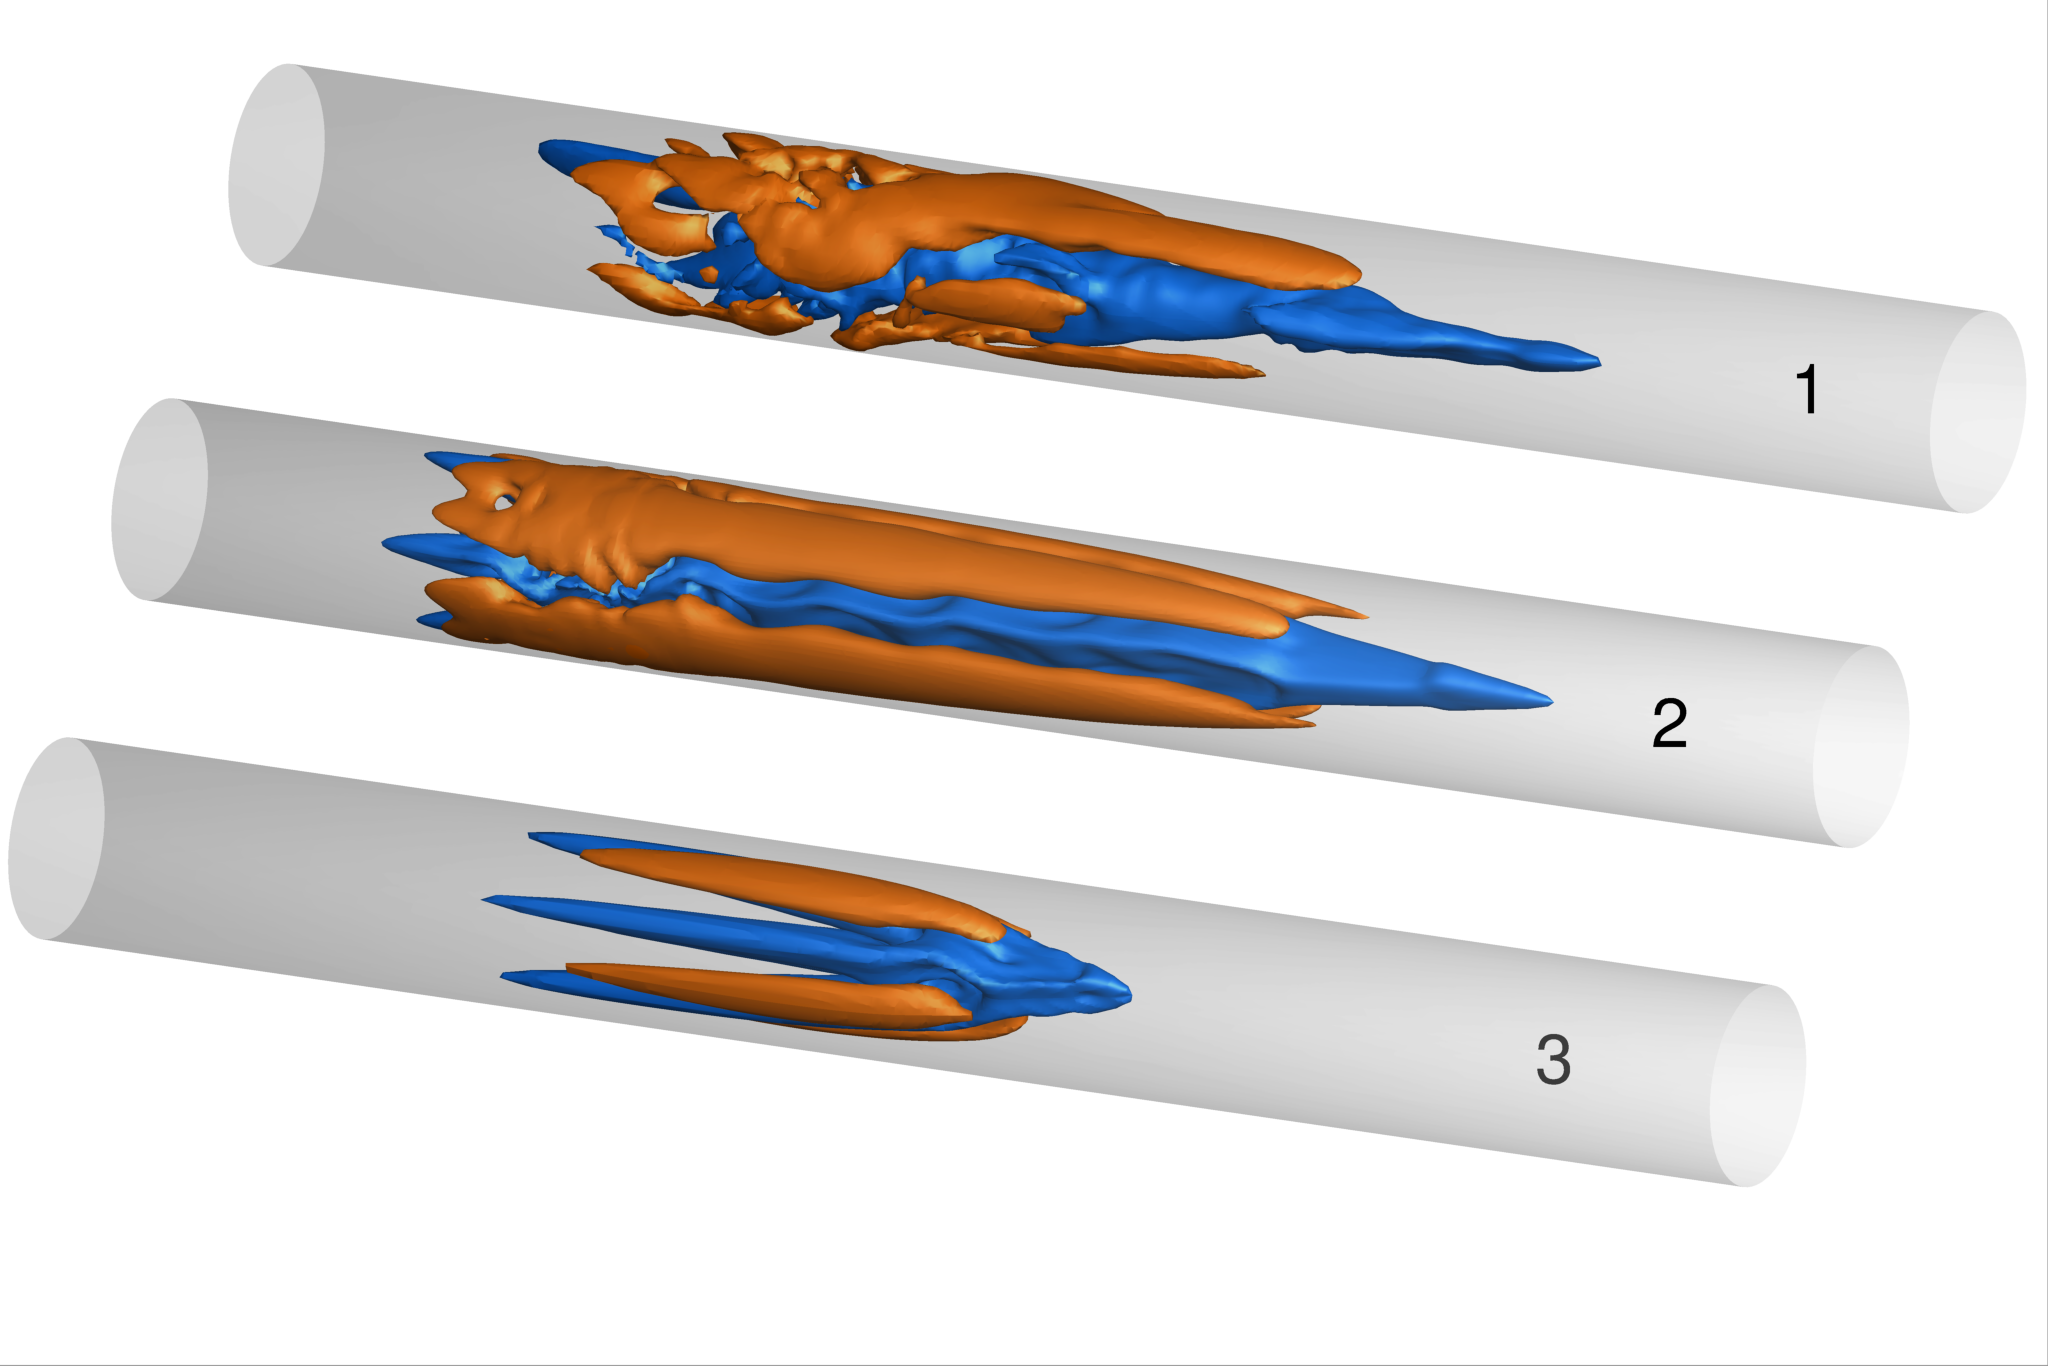
\includegraphics[width=1\linewidth]{3D_cmp.png}}
\caption{Визуализация численных расчетов турбулентных порывов: 1 --- $\Re = 2000$; 2 --- $\Re = 2000$ с учетом \eqref{sym_eq}, \eqref{per_eq}; 3 --- решение на сепаратрисе, $\Re = 2200$. Темным и светлым тоном выделены поверхности скорости $-0.1$ и $+0.1$ относительно скорости течения Пуазейля. Поток направлен слева направо.}
\label{3D_img}
\end{figure}

Предельное решение на сепаратрисе получено при $\Re=2200$. Условие \eqref{per_eq} при \eqref{sym_eq} порождает условие отражения относительно сечения $\theta = \pi/2$, аналогичное условию отражения относительно сечения $\theta = 0$:
\begin{equation} \label{sym2_eq}
(v_x, v_r, v_\theta)(x, r, \pi/2 + \theta, t) = (v_x, v_r, -v_\theta)(x, r, \pi / 2 - \theta, t).
\end{equation}
С учетом \eqref{sym_eq}, \eqref{sym2_eq} расчет проводился для четверти объема трубы $0\leqslant\theta\leqslant\pi/2$. Исходное решение найдено при $L_x = 80$ на сетке, содержащей $512 \times 32 \times  32$ ячеек в продольном, радиальном и угловом направлениях. 

Предварительно найденное турбулентное решение $\v_{turb}(\x,t)$ используется в итерационной процедуре отыскания предельного решения на сепаратрисе. Задача решается с начальным условием
\begin{equation} \label{edge_init_eq}
\v(\x,t=0) = \v_{Pois}(\x)+\alpha(\v_{turb}(\x,t=t_0) - \v_{Pois}(\x)).
\end{equation}
Здесь $\v_{Pois}=(1-r^2,0,0)$ --- течение Пуазейля, $t_0$ --- некоторый фиксированный момент времени, $\alpha \in [0,1]$ --- скалярный параметр. Значение $\alpha=0$ соответствует нулевому возмущению, и решением при $t > 0$ остается течение Пуазейля. Выбирая $\alpha=1$, уже в начальный момент времени реализуется турбулентный режим, который сохраняется при $t > 0$. При промежуточных значениях $\alpha$ происходит стремление решения либо к одному, либо к другому режиму. Применяя метод деления пополам, мы постепенно отыскиваем то значение $\alpha$, при котором решение эволюционирует на сепаратрисе, разделяющей области притяжения двух режимов течения. Суть метода состоит в том, что если при текущем значении $\alpha$ возмущения затухают, то на следующей итерации $\alpha$ увеличивается; если развивается турбулентный режим течения --- $\alpha$ уменьшается. На рисунке \ref{bisection_pic} представлены графики $A(t)$ – среднеквадратичного по всему объему отклонения поля скорости от течения Пуазейля для нескольких значений $\alpha$, демонстрирующие сходимость итерационного процесса. При уточнении значения $\alpha$ продлевается длительность балансирования решения на сепаратрисе.


\begin{figure}
\center{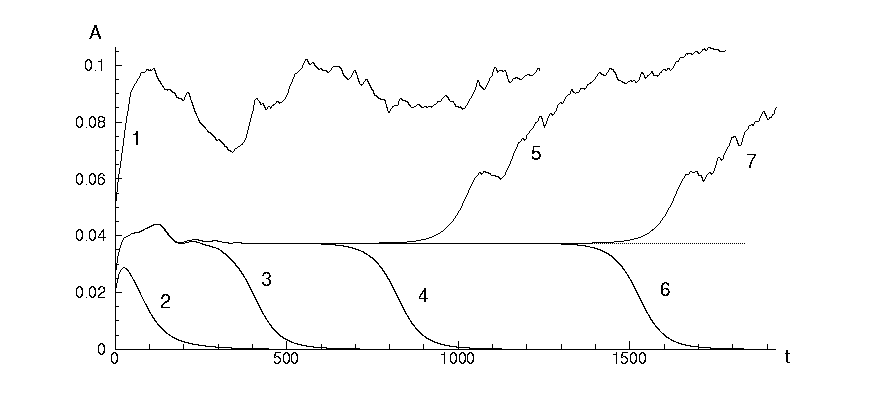
\includegraphics[width=1\linewidth]{bisection.png}}
\caption{Итерационный процесс построения решения на сепаратрисе. 1--7 --- эволюция среднеквадратичной амплитуды возмущений $A(t)$ при уточнении значения $\alpha$.}
\label{bisection_pic}
\end{figure}

С каждой новой итерацией решение проводит на сепаратрисе в среднем на 30 единиц времени больше. В расчетах для представления действительных числе использованы 64-битные числа с плавающей запятой. Это позволило найти около 50 приближений к решению на сепаратрисе. Соответственно, решение удалось удержать на сепаратрисе в течении приблизительно 1500 единиц времени. Из них ориентировочно первые 500 единиц происходит перестройка решения, после чего режим течения устанавливается. В согласии с результатами \cite{Avila2013}, решение на сепаратрисе при $\Re=2200$ постепенно выходит на условно периодический режим. Это решение описывает локализованной в пространстве структуры, которая сносится вниз по потоку с постоянной скоростью. В подвижной системе отсчета поле скорости в каждой точке испытывает периодические колебания. Для скорости сноса и периода колебаний получены значения $c=0.69$ и $T=60$ (в \cite{Avila2013} сообщается о $c=0.76$ и $T=60$). Во всех выполненных расчетах режим течения, устанавливающийся на сепаратрисе, не зависит от исходного турбулентного поля скорости $\v_{turb}$. 

\begin{comment}
Так как скорость сноса модельного порыва заранее не известна, решение на сепаратрисе было найдено в системе отсчета, двигающейся со скоростью $0.5$. После того, как решение на сепаратрисе найдено, изменить скорость перемещения системы отсчета уже не представляется возможным вследствие высокой чувствительности решения к возмущениям, возникающим в данном случае в результате неточностей численного интегрирования. Чтобы получить решение в сопутствующей системе отсчета, метод поиска решения на сепаратрисе применен повторно в системе отсчета, двигающейся с уже известной скоростью перемещения порыва. 
\end{comment}

Сравнение предельного решения на сепаратрисе с турбулентным порывом, представленное на рисунке \ref{3D_img}, показывает качественное согласие этих решений. Во всех структурах имеются протяженные области ускоренного и замедленного движения, концентрирующиеся в пристенной области трубы. Сохраняется и основная качественная особенность порыва --- медленное понижение осевой скорости на переднем фронте и более резкое её восстановление на заднем (смотри рисунок \ref{ucl_cmp_img}). Мы будем называть предельное решение на сепаратрисе {\it модельным порывом}.  

\begin{figure}
\center{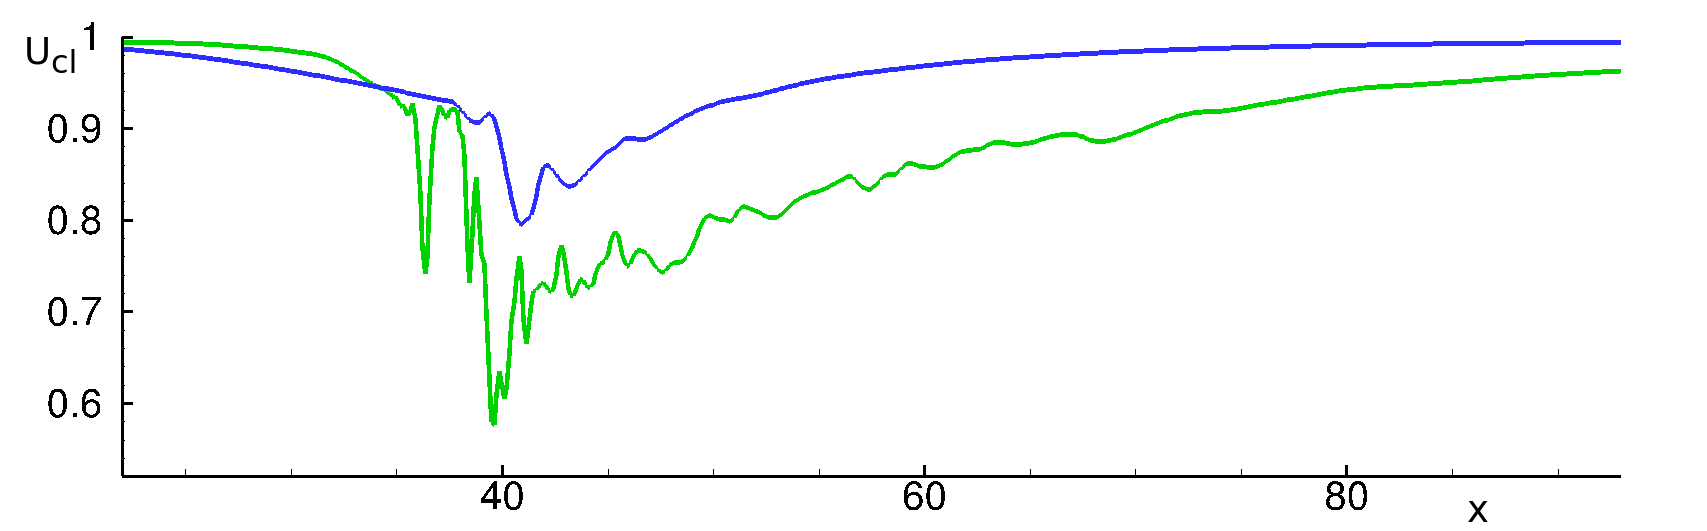
\includegraphics[width=0.7\linewidth]{ucl_cmp.png}}
\caption{Сравнение скорости на оси трубы в турбулентном (1) и модельном (2) порывах.}
\label{ucl_cmp_img}
\end{figure}

Для того, чтобы установить влияние условия периодичности вдоль трубы на предельное решение, решение было найдено в расчетной области вдвое большей протяженности, при $L_x = 160$ (число узлов сетки в продольном направлении также удвоено). Также при исходном значении $L_x = 80$ решение было получено на более подробной сетке, содержащей $1024 \times 64 \times 64$ ячеек (в сравнении с исходной сеткой в каждом направлении число ячеек удвоено). Результаты, полученные на трех сетках, качественно совпадают и количественно близки. Для сравнения, на рисунке \ref{amp_pic} представлены некоторые интегральные характеристики модельного порыва, полученные на различных сетках (подробное описание изображенных величин приведено в следующем разделе). Полученные результаты подтверждают достаточность расчетной сетки и длины расчетной области для адекватного воспроизведения модельного порыва, а также то, что его пространственная локализация не связана с условием периодичности вдоль трубы. Характеристики полученного модельного порыва согласуются с результатами работы \cite{Avila2013}. Это подтверждает, что найденное решение является решением математической задачи и не зависит от численного метода, которым оно было найдено. В работе \cite{Avila2013} решение получено двумя методами --- полностью спектральным \cite{Meseguer2007} и спектрально-конечно-разностным \cite{Willis2009}. Мы применяем конечно-разностный метод \cite{Nikitin2006}. Также, модельный порыв был воспроизведен в работе \cite{Chantry2014} спектрально-конечно-разностным методом \cite{Willis2009}; авторами также сообщается о совпадении результатов с \cite{Avila2013}. 


\section{Основные свойства модельного порыва} \label{edge_char_seq}

При $\Re=2200$ модельный порыв имеет длину около $40R$ и перемещается вдоль трубы со скоростью $c = 0.69U$. В подвижной системе отсчета он является периодическим по времени с периодом $T = 60 R/U$. Характерным свойством модельного порыва является наличие вытянутых вдоль потока областей с повышенным и пониженным значением продольной компоненты скорости, чередующихся в угловом направлении (смотри рисунок \ref{3D_img}). Полосы повышенной скорости целиком расположены около стенки трубы, полосы замедления соединяются в единое целое в приосевой области вблизи переднего фронта. Наличие вытянутых вдоль потока полос ускоренного и замедленного движения --- характерное свойство любого пристенного турбулентного течения. Однако, в отличие от реальной турбулентности, где полосы случайно блуждают во времени и в пространстве, в рассматриваемом решении полосы сохраняют свое положение и форму, лишь слегка искажаясь периодическими колебаниями. 

\begin{figure}
\center{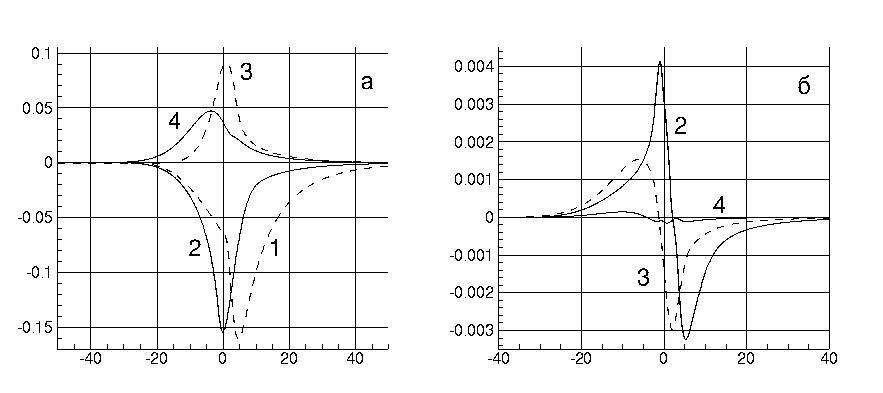
\includegraphics[width=1\linewidth]{U2D.png}}
\caption{Распределения вдоль трубы продольной (a) и радиальной (b) компоненты осесимметричной составляющей скорости $\V_{2D}$ для нескольких расстояний от оси трубы: 1–4 – r = 0, 0.4, 0.7, 0.9}
\label{U2D_pic}
\end{figure}

Для удобства перейдем в подвижную систему координат, перемещающуюся вдоль трубы со скоростью сноса локализованной структуры. В подвижной системе решение представляется в виде суперпозиции стационарной составляющей $\V(\x) = \overline{\v}^t$ и колебательной $\v_n(t,\x) = \v - \V$. Стационарную составляющую, в свою очередь, представим в виде суперпозиции осесимметричной $\V_{2D}(\x) = \overline{\V}^{\theta}$ и трехмерной $\V_{3D}(\x) = \V - \V_{2D}$ составляющих. Распределения продольной компоненты осесимметричной составляющей скорости вдоль трубы $V_{x,2D}(x)$ для нескольких расстояний от оси трубы представлены на рисунке \ref{U2D_pic}(а) (даны отклонения от течения Пуазейля). Начало системы отсчета $x=0$ помещено в сечение, в котором среднее отклонение скорости от течения Пуазейля максимально. Голова структуры, где начинает проявляться отклонение осевой скорости, располагается на расстоянии $x \approx 45$. Хвостовая часть структуры на сепаратрисе очерчена не так четко, как в турбулентных порывах, где восстановление скорости происходит на отрезке длиной в $3-5$ радиусов трубы.  Падение скорости в приосевой области трубы компенсируется ускорением у стенки. Поведение радиальной компоненты $V_{r,2D}$, показанное на рисунке \ref{U2D_pic}(b), соответствует изменению осевой скорости --- в зоне замедления на оси происходит растекание жидкости к стенкам, $V_{r,2D}>0$, в передней части происходит обратный процесс и $V_{r,2D}<0$.

\begin{figure}
\center{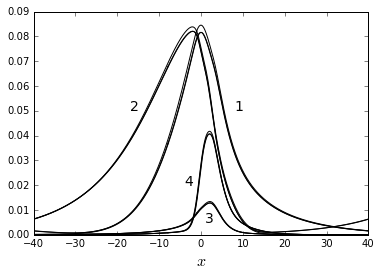
\includegraphics[width=0.6\linewidth]{amp.png}}
\caption{Распределения вдоль трубы среднеквадратичных по сечению амплитуд трех составляющих движения: 1 -- $\V_{2D}$ (отклонение от течения Пуазейля); 2, 3 -- продольная и поперечные компоненты скорости $\V_{3D}$; 4 -- $\v_{n}$. Представлены результаты, полученные на трех расчетных сетках, параметры которых приведены в разделе \ref{edge_seq}. }
\label{amp_pic}
\end{figure}

На рисунке \ref{amp_pic} приведены распределения по $x$ среднеквадратичных по сечению трубы амплитуд трех составляющих движения: стационарной осесимметричной (отклонение от течения Пуазейля) $A_{2D}$, стационарной трехмерной $A_{3D}$ и колебательной $A_n$. Распределение $A_{2D}(x)$ соответствует рисунку \ref{U2D_pic}. Отклонение от течения Пуазейля заметно на значительном отрезке от $x=-30$ до $x=40$. Максимум $A_{2D}$ составляет 8.4\%. Величина $A_{3D}$ характеризует интенсивность полосчатых структур. Как видно на рисунке~\ref{3D_img}, полосчатые структуры появляются на некотором расстоянии вверх по потоку от головы порыва и сохраняются на значительном расстоянии позади него. В соответствии с этим $A_{3D}(x)$ имеет выраженную асимметрию относительно точки $x=-2$, где эта величина достигает максимума. Интенсивность полос быстро падает вниз по потоку и сохраняется на значительном расстоянии в верхней части потока. В отличие от стационарных полосчатых структур, колебательная составляющая движения сосредоточена на сравнительно непротяженном отрезке трубы от $x=-5$ до $x=15$ с максимальной амплитудой в 4\% при $x=2.5$.


\begin{figure}[h]
\center{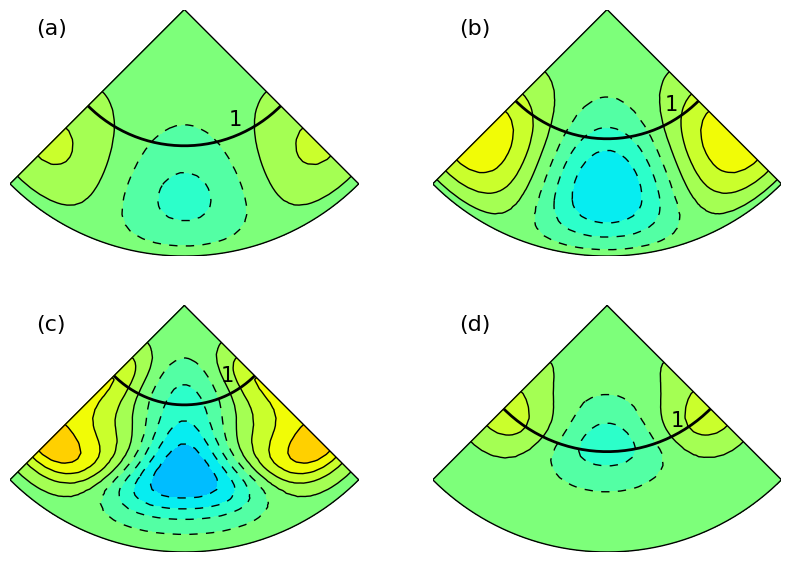
\includegraphics[width=0.8\linewidth]{V3D_cs.png}}
\caption{Распределения продольной составляющей $V_{x,3D}$ в нескольких сечениях трубы: (a)--(d) --- $x = -20, -10, 0, 5$. Сплошные изолинии --- положительная скорость, пунктирные изолинии --- отрицательная скорость, 1 --- линия, на которой относительная скорость жидкости равна нулю ($V_{x} = c$).}
\label{V3D_cs_pic}
\end{figure}


В трехмерную стационарную составляющую движения $\V_{3D}$ попадают полосы повышенной и пониженной скорости. Поле $V_{x,3D}$ в нескольких сечениях трубы изображено на рисунке~\ref{V3D_cs_pic}. В каждом сечении трубы полосы пониженной скорости ($V_{x,3D} < 0$) проходят через центр расчетной области, при $\theta = \pi/4$. Полосы повышенной скорости ($V_{x,3D} > 0$) попадают на границы расчетной области в угловом направлении, находящиеся при $\theta = 0, \pi/2$. Среднее поле скорости оказывается симметрично относительно плоскости, проходящей через центр расчетной области при $\theta = \pi/4$, так как поле скорости решения на сепаратрисе $\v = (v_x, v_r, v_\theta)$ имеет дополнительную симметрию отражения относительно указанной плоскости со сдвигом на половину периода по времени:
\begin{equation}
(v_x, v_r, v_\theta)(x, r, \pi/4 + \theta, t) = (v_x, v_r, -v_\theta)(x, r, \pi/4 - \theta, t + T/2). 
\end{equation} 


\begin{figure}[h]
\center{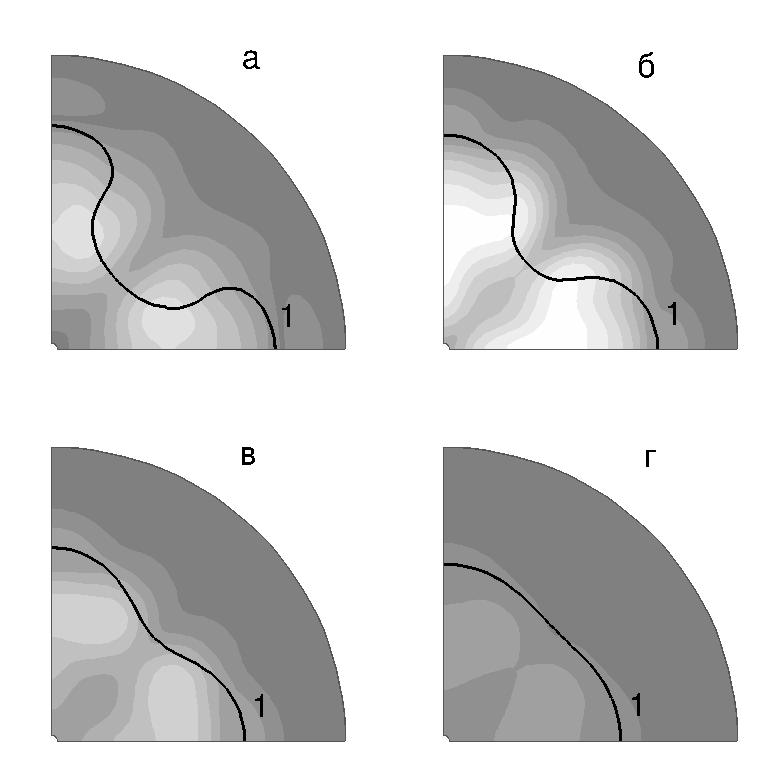
\includegraphics[width=0.8\linewidth]{puls_cs.png}}
\caption{Изолинии среднеквадратичной амплитуды колебаний в нескольких сечениях трубы: (a)--(d) --- x = 0, 2.5, 5, 7.5. В пристенной области амплитуда колебаний близка к нулю. 1 --- линия, на которой относительная скорость жидкости равна нулю ($V_{x} = c$).}
\label{puls_cs_pic}
\end{figure}

Распределения среднеквадратичной амплитуды пульсационной составляющей движения $\v_n$ в нескольких сечениях трубы приведены на рисунке \ref{puls_cs_pic}. Пульсации имеют существенную амплитуду между полосами повышенной и пониженной скорости, а также между полосой ускорения и осью трубы. Пульсационная составляющая движения $\v_n$ по форме напоминает бегущую волну. Её фазовая скорость близка к $0.77U$, что на $0.08U$ выше скорости перемещения порыва. Длина бегущей волны несколько меняется по мере продвижения вниз по потоку. Её можно оценить в $5R$. 


\section{Механизм поддержания полос повышенной и пониженной скорости} 

Все описанные составляющие движения находятся в динамическом взаимодействии друг с другом. Как видно на рисунке \ref{amp_pic} наиболее локализованной вдоль трубы оказывается колебательная составляющая. Доминирующая мода колебательной составляющей пропорциональна $e^{2\pi it/T}$ во времени и $e^{2i\theta}$ в угловом направлении. Нелинейное взаимодействие колебательных мод порождает колебания на высших частотах, а также дает вклад в стационарную составляющую движения. В стационарной составляющей кроме осесимметричной части доминирует мода, пропорциональная $e^{4i\theta}$, обладающая $\pi/2$-периодичностью в угловом направлении. Именно такой периодичности по углу соответствуют четыре пары полосчатых структур, наблюдающихся при решении задачи с условиями \eqref{sym_eq}, \eqref{per_eq}.

Отметим, что непосредственный вклад колебаний в образование полос не велик. Основной механизм роста полос это так называемый лифтап (<<lift-up>>) эффект, связанный с появлением движения в перпендикулярной к основному потоку плоскости. Частицы жидкости, перемещающиеся от стенки в сторону оси трубы, приносят дефект скорости и образуют полосу замедления, а частицы, двигающиеся в противоположном направлении --- от оси к стенке, образуют полосу ускорения. Основная роль колебательной составляющей в этом механизме состоит именно в порождении стационарного движения в поперечной плоскости, распределение среднеквадратичной амплитуды которого $A_{\perp}(x)$ также представлено на рисунке \ref{amp_pic} кривой 3. Как видно, область сосредоточения поперечного движения практически совпадает с областью существования колебаний. Некоторое уклонение $A_{\perp}(x)$ вверх по потоку объясняется конвективным переносом этого движения (поперечное движение в основном возникает в периферийной части сечения трубы, где скорость потока в выбранной системе отсчета отрицательна).

\begin{figure}[h]
\center{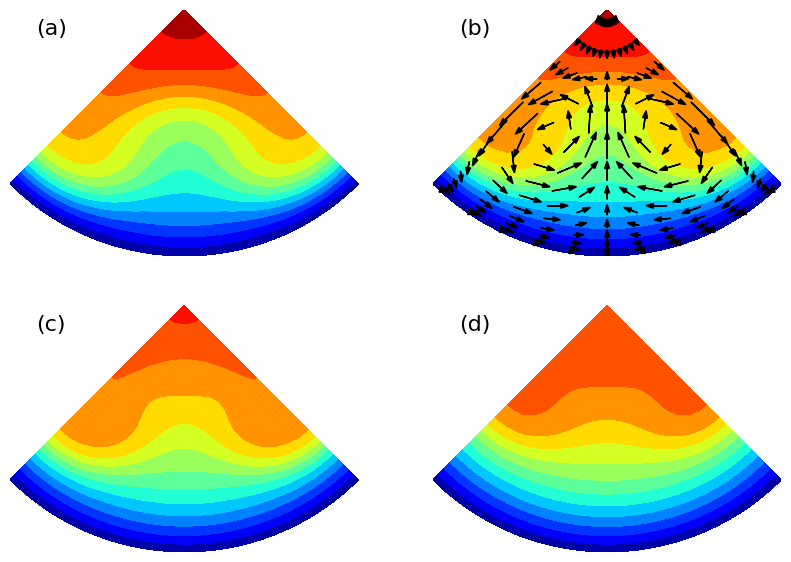
\includegraphics[width=1\linewidth]{VEL_cs.png}}
\caption{Среднее поле скорости $\V$: ряд (a) --- поперечная компонента, ряд~(b)~--- изолинии продольной компоненты. На стенке скорость жидкости равна нулю. Изображено три сечения трубы, $x = 0, 2.5, 5$.}
\label{VEL_cs_pic}
\end{figure}

На рисунке \ref{VEL_cs_pic} приведены поперечная $(V_r, V_\theta)$ и продольная $V_x$ компоненты стационарного течения в области, где пульсации имеют существенную амплитуду. Стационарное поперечное течение соответствует существованию в потоке стационарных продольных вихрей, поддерживающих существование полос. Там, где стационарное поперечное движение направлено от стенки к оси трубы, находятся полосы замедления. Там, где поперечное движение направлено к стенки --- полосы ускорения. 

Формирующиеся в области небольшой протяженности полосчатые структуры переносятся в переднюю и заднюю часть порыва за счет конвекции. На рисунке \ref{V3D_cs_pic} на линии 1 средняя продольная скорости $V_x$ в системе отсчета, связанной с порывом, равна нулю. В приосевой области, ограниченной этой линией, скорость положительна, а в периферийной --- отрицательна. Видно, что полосчатые структуры во всех сечениях (кроме переднего, x = 5) располагаются в области отрицательной относительной скорости. Среднее течение с отрицательной скоростью переносит полосчатые структуры в заднюю часть порыва, где они формируют картину, похожую на вытянутые щупальца медузы (смотри рисунок \ref{3D_img}). При $x > 5$ полосчатые структуры концентрируются в приосевой части трубы и конвектируются вперед положительной скоростью относительного движения, благодаря чему в передней части порыва $A_{3D}$ сохраняет заметную величину, несмотря на отсутствие поперечного движения.


\section{Механизм возбуждения пульсаций}

\begin{figure}
\center{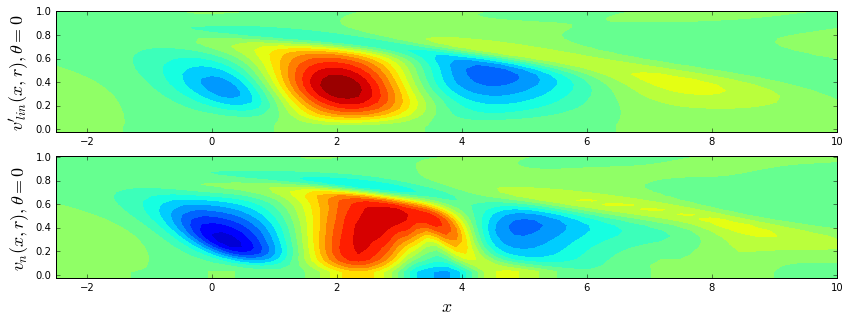
\includegraphics[width=1\linewidth]{lin_ls_cmp.png}}
\caption{Сравнение мгновенного поля продольной скорости пульсаций, возникающих в рамках линеаризованных уравнений, $\v'_1$ (a) и пульсационной составляющей движения $\v_n$ (b) в сечении $\theta = 0$. Сплошные изолинии --- положительные значения, прерывистые --- отрицательные.}
\label{lin_ls_cmp_pic}
\end{figure}

Полосчатые структуры достигают максимальной амплитуды в области $x\in[-5,0]$, где создаются условия для возникновения колебаний. Наиболее вероятный механизм генерации колебаний --- механизм потери устойчивости стационарной составляющей течения. Для проверки этой гипотезы стационарное течение $\V$ было исследовано на устойчивость к малым возмущениям $\v'$. Предположение малости $\v'$ позволяет линеаризовать уравнения. Линеаризованные относительно $\v'$ уравнения Навье-Стокса в подвижной системе координат, связанной с порывом, имеют вид:
\begin{equation} \label{lin_eq}
\frac{\partial \v'}{\partial t} = c \frac{\partial \v'}{\partial x} - (\V \cdot \nabla) \v' - (\v' \cdot \nabla) \V - \nabla p' + \nu \nabla^2 \v'. 
\end{equation}
Здесь $p'$ -- пульсационная составляющая давления. Расход $\v'$ равен нулю. Другие уравнения в постановке задачи линейные и для $\v'$ имеют тот же вид, что и для $\v$. Задача решается с дополнительными условия симметрии \eqref{sym_eq}, \eqref{per_eq}, которым удовлетворяет поле скорости модельного порыва. 

Линеаризованные относительно возмущений уравнения с некоторыми случайными начальными условиями интегрировались по времени до выхода решения на режим экспоненциального изменения. Обнаружено, что действительно поле скорости $\V$ неустойчиво к малым возмущениям. Растущее возмущение $\v'_1 \sim e^{(\lambda+i\omega)t}$ имеет инкремент нарастания $\lambda=0.012$ и частоту $\omega=0.116$, близкую к частоте колебаний $2\pi/60=0.105$ в решении на сепаратрисе. Что более существенно, поле скорости растущего решения $\v'_1$ качественно повторяет основные особенности поля скорости пульсационной составляющей движения модельного порыва $\v_n$. В качестве подтверждения на рисунке \ref{lin_ls_cmp_pic} представлены мгновенные поля скорости $\v'_1$ и $\v_n$ в продольном сечении $\theta = 0$. Моменты времени подобраны так, что фазы решений совпадают. Также на рисунке \ref{lin_amp_cmp_pic} для сравнения представлены амплитуды $\v_1'$ и $\v_n$ в нескольких сечениях трубы. Нет сомнений, что колебания возникают в результате линейной неустойчивости стационарной составляющей движения. Решение линейной задачи обладает дополнительной симметрией отражения относительно плоскости $\theta = \pi/4$, выражаемой формулой:
\begin{equation} \label{dop_sym_eq}
(-v_x, -v_r, v_\theta)(x, r, \pi/4 + \theta, t) = (v_x, v_r, v_\theta)(x, r, \pi/4 - \theta, t). 
\end{equation} 
В целом, поле $\v'_1$ имеет более простую форму, чем $\v_n$. В частности, $\v'_1$ меняется во времени по гармоническому закону. Простота формы $\v'_1$ делает его предпочтительным объектом при исследовании механизмов влияния пульсаций на среднее течение. 


\begin{figure}
\center{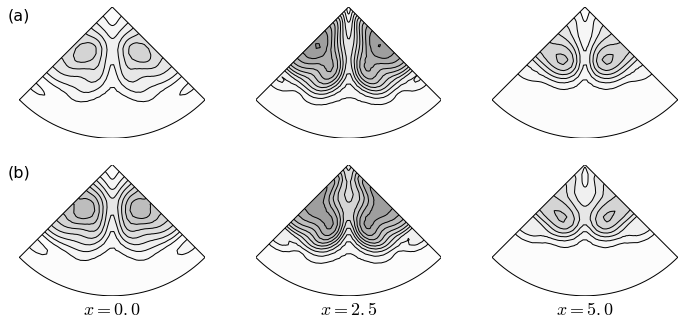
\includegraphics[width=1\linewidth]{lin_amp_cmp.png}}
\caption{Сравнение амплитуды пульсаций, возникающих в рамках линеаризованных уравнений, $\v'_1$ (ряд (a)) и пульсационной составляющей движения $\v_n$ (ряд (b)) в нескольких сечения трубы, $x = 0, 2.5, 5$. Вблизи стенки амплитуда пульсаций близка к нулю.}
\label{lin_amp_cmp_pic}
\end{figure}

В реальном течении пульсационная составляющая движения имеет конечную амплитуду и нелинейными слагаемыми в уравнении, описывающем эволюцию пульсаций, уже нельзя пренебрегать. По-видимому, роль нелинейных слагаемых сводится к тому, что они несколько меняют форму пульсаций так, что рост амплитуды пульсационной составляющей движения прекращается. При этом, именно линейные слагаемые определяют форму пульсаций и ответственны за передачу энергии в пульсационную составляющую движения. 

Отметим, что точки максимального роста колебаний находятся на линии, соответствующей нулевой относительной скорости (линия 1 на рис.~\ref{puls_cs_pic}). По этой причине область порождения колебаний остается неподвижной относительно порыва. Интересно, что в этой же области ($x = 0,\ r \approx 0.4$) происходит смена знака радиальной компоненты осесимметричной составляющей скорости (смотри рисунок~\ref{U2D_pic}(b)). При $x<0$ радиальная скорость положительна, поэтому колебания, возникшие в задней части порыва, относятся в сторону стенки трубы, где относительная скорость отрицательна, и продолжают двигаться вверх по течению. Наоборот, при $x>0$ радиальная скорость направлена к оси трубы. Туда же, в область положительной скорости, сносятся и колебания, обнаруживающиеся в передней части порыва.

Отметим также, что неустойчивость полосчатых структур является неотъемлемой составляющей всех сценариев самоподдержания турбулентности в пристенных течениях. В некоторых работах предполагается, что неустойчивость возникает в пристенных областях полос замедленного движения, где в локальном профиле скорости $V_x(r)$ на фоне наибольшего градиента появляется точка перегиба --- источник неустойчивости в механизме типа Кельвина--Гельмгольца. В частности, именно такой механизм предлагается в качестве механизма возникновения колебаний в турбулентном порыве в \cite{Shimizu2009}. В рассматриваемом нами решении на сепаратрисе это определенно не так. Как видно на рисунке~\ref{puls_cs_pic} в сечении $x=0$, соответствующем максимальной скорости роста колебаний, амплитуда колебаний минимальна как раз в области полосы замедления ($\theta=\pi/4$). Наибольшие колебания развиваются наоборот вблизи полос ускорения, а если быть более точным, в промежуточных областях между полосами. В этих областях стационарная составляющая скорости течения претерпевает наибольшее изменение и имеет точки перегиба, но не как функция радиальной переменной, а как функция угла.



\section{Влияние продольной неоднородности стационарной составляющей движения на форму пульсаций}

Замечено, что в модельном порыве область наибольшей интенсивности пульсаций совпадает с областью резкого падения скорости на его заднем фронте (см. рис. \ref{ucl_cmp_img}, \ref{amp_pic}). Аналогичная особенность отмечена в турбулентном порыве \cite{Hof2010}. Чтобы оценить роль продольной неоднородности среднего течения в процессе формирования пульсаций, в работе выполнен анализ устойчивости однородных вдоль трубы полей скорости $\U_i = \V\big|_{x=x_i}$, повторяющих среднее поле скорости модельного порыва $\V$ в сечениях трубы $x = x_i$. Значения $x_i$, при которых было выполнено исследование поля скорости $\U_i$, принадлежат интервалу $(-8,4)$, где пульсационная составляющая движения получает энергию от среднего течения и имеет существенную амплитуду. Поля скорости $\U_i$ имеют полосчатую структуру и воспроизводят неоднородность среднего поля скорости по координатам $r$ и $\theta$, но теряют неоднородность среднего течения по координате $x$. Сравнение характеристик устойчивости полей скорости $\V$ и $\U_i$ позволяет делать выводы о роли продольной неоднородности в процессе формирования пульсаций. 

Собственные решения линейной задачи устойчивости однородного вдоль трубы поля скорости имеют вид $\v' = \mathrm{Real}\left(\hat \v (r, \theta, t) e^{i \alpha x}\right)$, где функция $\hat \v$ имеет комплексные значения, функция $\mathrm{Real}(z)$ имеет значение действительной части комплексного числа $z$. Постановка задачи линейной устойчивости однородного вдоль трубы поля скорости формулируется относительно $\hat \v$ и является двумерной (пропадает зависимость от $x$). Задача имеет дополнительный параметр $\alpha > 0$, характеризующий волновое число возмущения, устойчивость к которому анализируется. В этой постановке уравнения движения в системе координат, перемещающейся вдоль трубы со скоростью $c$, и уравнение неразрывности имеют вид: 
\begin{equation} \label{hat_NS_eq}
\frac{\partial \hat \v}{\partial t} = i \alpha  c \hat \v - (\U_i \cdot \hat \nabla) \hat \v - (\hat \v \cdot \nabla) \U_i - \hat \nabla \hat p + \nu \hat \nabla^2 \hat \v,
\end{equation}
\begin{equation} \label{hat_div_eq}
\hat \nabla \cdot \hat \v = 0,
\end{equation}
где функция $\hat p = \hat p(r,\theta,t)$ имеет комплексные значения, $p' = \mathrm{Real}\left(\hat p e^{i \alpha x}\right)$ --- пульсационная составляющая давления, оператор $\hat \nabla$ имеет вид: 
\begin{equation*}
\hat \nabla = \left( i\alpha, \frac{\partial}{\partial r}, \frac{\partial}{r \partial \theta} \right).
\end{equation*}
На стенках трубы ставится условие прилипания. На решение накладываются дополнительные условия симметрии \eqref{sym_eq}, \eqref{per_eq}, при которых найден модельный порыва. Условие периодичности вдоль потока \eqref{bc2_eq} снимается. 

\begin{figure}
\center{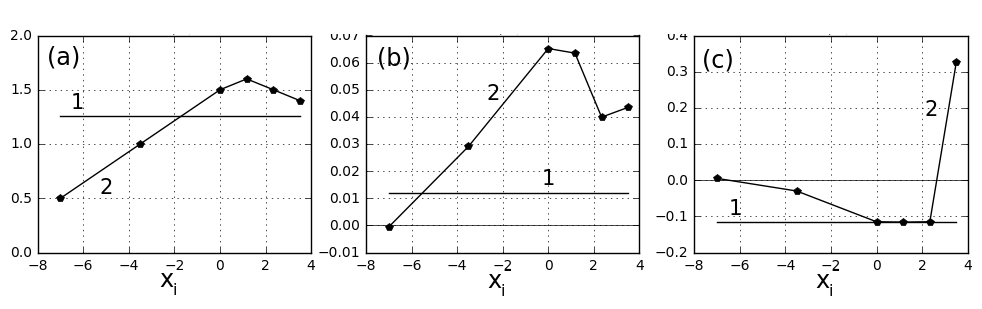
\includegraphics[width=1\linewidth]{cs_lin.png}}
\caption{Значение волнового числа $\alpha$ (a), инкремента нарастания $\lambda$ (b) и угловой частоты $\omega$ (в системе отсчета порыва) (c) для наиболее быстро растущего возмущения поля скорости модельного порыва $\V$ (линия 1) и однородных вдоль потока полей скорости $\U_i$, повторяющих $\V$ в сечении $x = x_i$ (точки на линии 2).}
\label{cs_lin_pic}
\end{figure}

На устойчивость исследованы поля скорости $\U_i = \V\big|_{x=x_i}$ для $x_i = -7.1,$ $-3.5, 0, 1.2, 2.3, 3.5$.  Для каждого исследованного $\U_i$ среди собственных решений линейной задачи устойчивости с различными значениями волнового числа $\alpha >0$ найдено наиболее быстро растущее (медленно затухающее). Наиболее быстро растущее (медленно затухающее) собственное решение линейной задачи устойчивости поля скорости $\U_i$ при фиксированном значении $\alpha$ получено интегрированием уравнений \eqref{hat_NS_eq}, \eqref{hat_div_eq} со случайными начальными данными до выхода на экспоненциальный режим роста, $||\hat \v|| \sim e^{(\lambda + i\omega) t}$. 

На рисунке \ref{cs_lin_pic} приведены полученные значения волнового числа $\alpha$, инкремента нарастания $\lambda$ и угловой частоты $\omega$ для наиболее быстро растущих (медленно затухающих) возмущений поля скорости $\U_i$, как функции $x_i$ (точки на линии 2). Также на рисунке (линией 1) приведены характеристики наиболее быстро растущего возмущения стационарной составляющей поля скорости модельного порыва $\V$ (значение длины волны приблизительное). Угловая частота приведена в системе отсчета, перемещающейся со скоростью порыва. 

Поля скорости $\U_i$ при $x_i \in (-4,4)$ оказываются неустойчивыми, причем скорость роста наиболее быстро растущего возмущения оказывается выше скорости роста возмущений стационарной составляющей движения модельного порыва $\V$. Наибольшей скоростью роста обладают возмущения полей скорости $\U_i$ при $x_i \in (0, 2)$. Следствием этого факта может быть то, что именно при $x \in (0,2)$ пульсационная составляющая движения $\v_n$ достигает наибольшей амплитуды (см. рис. \ref{amp_pic}). Наиболее быстро растущие  возмущения полей скорости $\U_i$ при $x_i \in (0,3)$ повторяют форму пульсационной составляющей движения модельного порыва. В частности, их волновые числа и угловые частоты близки к соответствующим значениям как для наиболее быстро растущих возмущений поля скорости $\V$, так и для пульсационной составляющей движения модельного порыва $\v_n$. Распределения по сечению трубы амплитуды колебаний для наиболее быстро растущих возмущений полей скорости $\U_i$ при $x_i \in (0,3)$, приведенные на рисунке \ref{cs_lin_map_pic}, повторяют распределение амплитуды колебаний в модельном порыве (см. рис. \ref{puls_cs_pic}).


\begin{figure}
\center{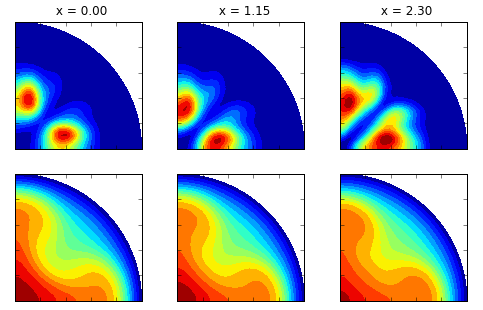
\includegraphics[width=1\linewidth]{cs_lin_map.png}}
\caption{Изолинии амплитуды колебаний для наиболее быстро растущего возмущения однородного вдоль трубы поля скорости $\U_i$ (a) и изолинии продольной компоненты поля скорости $\U_i$ (b), $x_i = 0, 1.2, 2.3$.}
\label{cs_lin_map_pic}
\end{figure}

Если при $x_i \in (0,3)$ наиболее быстро растущее возмущения полей скорости $\U_i$ повторяют качественные особенности пульсационной составляющей движения модельного порыва, то уже при $x_i = 3.5$ наиболее быстрорастущим оказывается возмущение принципиально другой формы. С этим, в частности, связано резкое отличие значения угловой частоты $\omega$, полученного при $x_i = 3.5$, от значений, полученных при меньших $x_i$ (см. рис. \ref{cs_lin_pic}). 

Среди исследованных однородных вдоль трубы полей скорости, имеющих полосчатую структур, найдены неустойчивые, для которых наиболее быстрорастущие возмущения воспроизводят как качественные, так и количественные характеристики пульсационной составляющей движения модельного порыва и имеют даже большую скорость роста, чем наиболее быстрорастущие возмущение средней составляющей движения модельного порыва. Таким образом, может быть сделан вывод, что продольная неоднородность стационарной составляющей движения не является необходимым условием для возникновения пульсаций. Образование пульсаций связано с неоднородностью стационарной составляющей движения в поперечной плоскости. 


\section{Взаимодействие между компонентами движения модельного порыва}

В предыдущих разделах были выделены компоненты движения модельного порыва и основные механизмы взаимодействия между ними. Компоненты движения находятся в динамическом равновесии, поддерживая существование друг друга и, следовательно, самого порыва. Более строго обосновать полученные результаты позволяет анализ баланса кинетической энергии в системе. Вклад каждой из компонент движения в производство кинетической энергии других компонент движения может быть вычислен на основе уравнений движения, и, в зависимости от его величины, могут быть сделаны выводы о положительном или отрицательном влиянии одних компонент движения на другие. 

Ниже приведен вывод уравнений баланса кинетической энергии для каждой компоненты движения. 
Осреднение уравнения Навье-Стокса по времени в системе отсчета, связанной с порывом, дает уравнение баланса импульса стационарной составляющей движения $\V = \overline{\v}^t$:
\begin{equation} \label{VEL_eq}
\pd{\V}{t} = c \pd{\V}{x} - (\V \cdot \nabla) \V - \overline{(\v_n \cdot \nabla) \v_n}^t - \nabla P + \nu \nabla^2 \V.
\end{equation}
Здесь $c$ --- скорость перемещения порыва, $P$ --- стационарная составляющая давления, $\v_n$ --- пульсационная составляющая скорости, черта над выражением с индексом $t$ обозначает осреднение по времени. Формально производная по времени от стационарной составляющей движения равна нулю, однако слагаемое $\partial \V/ \partial t$ сохранено в записи уравнения \eqref{VEL_eq} для удобства восприятия. В сравнении с уравнением Навье-Стокса в \eqref{VEL_eq} возникает новое слагаемое $-\overline{(\v_n, \nabla) \v_n}^t$, выражающее влияние пульсационной составляющей движения на среднее течение. 

Последующее осреднение \eqref{VEL_eq} по угловой координате дает уравнения баланса импульса двумерной компоненты движения $\V_{2D} = \overline{\V}^\theta$:
\begin{multline} \label{V2D_eq}
\pd{\V_{2D}}{t} = c \pd{\V_{2D}}{x} - (\V_{2D} \cdot \nabla) \V_{2D} - \overline{(\V_{3D} \cdot \nabla) \V_{3D}}^{\theta} - \overline{(\v_n \cdot \nabla) \v_n}^{t,\theta} - \\ - \nabla P_{2D} + \nu \nabla^2 \V_{2D}.
\end{multline}
Здесь $P_{2D} = \overline{P}^{\theta}$ --- двумерная составляющая давления, $\V_{3D} = \V - \V_{2D}$ --- трехмерная составляющая скорости, черта над выражением с индексом $\theta$ --- осреднение по угловой переменной. Вычитание \eqref{V2D_eq} из \eqref{VEL_eq} дает уравнение баланса импульса трехмерной составляющей движения $\V_{3D}$:
\begin{multline} \label{V3D_eq}
\pd{\V_{3D}}{t} = c \pd{\V_{3D}}{x} - (\V_{3D} \cdot \nabla) \V_{3D} - (\V_{3D} \cdot \nabla) \V_{2D} - (\V_{2D} \cdot \nabla) \V_{3D} + \\ + \overline{(\V_{3D} \cdot \nabla) \V_{3D}}^{\theta} - \overline{(\v_n \cdot \nabla) \v_n}^{t} + \overline{(\v_n \cdot \nabla) \v_n}^{t, \theta} - \nabla P_{3D} + \nu \nabla^2 \V_{3D}.
\end{multline}
Здесь $P_{3D} = P - P_{2D}$ --- трехмерная составляющая давления. Проектирование уравнения \eqref{V3D_eq} на ось $x$ дает уравнение, описывающее баланс импульса составляющей движения $\V_S = (V_{x,3D}, 0, 0)$, ассоциированной с полосами повышенной и пониженной скорости. Проектирование уравнения \eqref{V3D_eq} на поперечное сечение трубы дает уравнение баланса импульса составляющей движения $\V_V = (0, V_{r,3D}, V_{\theta,3D})$, ассоциированной с продольными вихрями. 
%Стоит отметить, что $\V_{2D}, \V_{3D}, \v_n$ удовлетворяют условию несжимаемости \eqref{eq0_Re}, в то время как $\V_S$ и $\V_V$ не удовлетворяют ему. 

\begin{figure}
\center{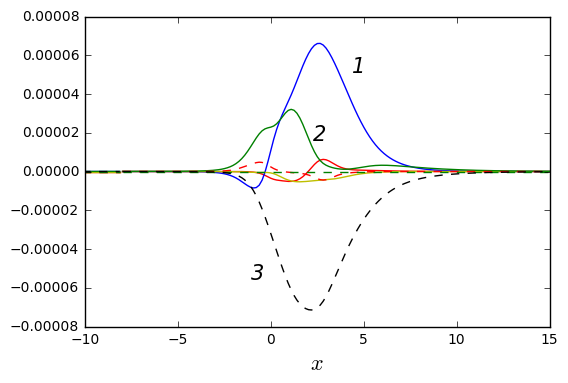
\includegraphics[width=0.6\linewidth]{e1_parts.png}}
\caption{Вклад в производство кинетической энергии пульсационной составляющей движения со стороны: 1 --- $\V_S$; 2 --- $\V_{2D}$; 3 --- вязких слагаемых. Другие слагаемые существенного вклада не дают.}
\label{e1_parts_pic}
\end{figure}

Вычитание \eqref{VEL_eq} из \eqref{NS_eq} дает уравнение эволюции пульсационной составляющей движения $\v_n$: 
\begin{multline} \label{vel1_eq}
\pd{\v_n}{t} = c \pd{\v_n}{x} - (\v_n \cdot \nabla) \v_n + \overline{(\v_n \cdot \nabla) \v_n}^t - (\V_{2D} \cdot \nabla) \v_n - (\V_S \cdot \nabla) \v_n - (\V_V \cdot \nabla) \v_n - \\ - (\v_n \cdot \nabla) \V_{2D} - (\v_n \cdot \nabla) \V_S - (\v_n \cdot \nabla) \V_V - \nabla p_n + \nu \nabla^2 \v_n. 
\end{multline}
Здесь $p_n = p - P$ --- пульсационная составляющая давления, среднее поле скорости представлено в виде суммы компонент движения $\V = \V_{2D} + \V_S + \V_V$, которые оказывают влияние на пульсационную составляющую движения через соответствующие нелинейные слагаемые. Осреднение по времени \eqref{vel1_eq}, умноженного на $\v_n$, дает уравнение изменения кинетической энергии пульсационной составляющей движения $e_n = \overline{\v_n^2/2}^t$: 
\begin{equation}\label{en_eq}
\pd{e_n}{t} = D_n^{2D} + D_n^{S} + D_n^{V} - \overline{\v_n (\v_n \cdot \nabla) \v_n}^t - \overline{\v_n \cdot \nabla p_n}^t + \nu \overline{\v_n \cdot \nabla^2 \v_n}^t,
\end{equation}
где слагаемые $D_n^{2D}$, $D_n^{S}$ и $D_n^{V}$ выражают генерацию $e_n$, обусловленную нелинейным взаимодействием $\v_n$ с компонентами движения $\V_{2D}$, $\V_S$ и $\V_V$, соответственно. Значения $D_n^{2D}$, $D_n^{S}$, $D_n^{V}$ вычисляются по формулам:
$$
D_n^{2D} = c \pd{e_n}{x}  - (\V_{2D} \cdot \nabla) e_n - \overline{\v_n (\v_n \cdot \nabla) }^t \V_{2D},
$$
$$
D_n^{S}  = - (\V_S \cdot \nabla) e_n - \overline{\v_n (\v_n \cdot \nabla)}^t \V_S,
$$
$$
D_n^{V} =  - (\V_V \cdot \nabla) e_n - \overline{\v_n (\v_n \cdot \nabla)}^t \V_V.
$$

На рисунке \ref{e1_parts_pic} приведены графики усреднённых по сечению трубы слагаемых из правой части уравнения \eqref{en_eq}. Наибольший вклад в генерацию кинетической энергии пульсаций $e_n$ дает слагаемое $D_n^S$ (кривая 1), что согласуется с представлениями о возникновении пульсаций вследствие линейной неустойчивости полосчатого движения. Хотя и не определяющий, но существенный положительный вклад дает слагаемое $D_n^{2D}$ (кривая 2). Так как течение $e_n$ не меняется во времен, сумма всех слагаемых в правой части уравнения \eqref{en_eq} равна нулю. Положительный вклад в генерацию $e_n$ со стороны $D_n^S$ и $D_n^{2D}$ компенсируется вязким слагаемым (кривая 3). Влияние других слагаемых оказывается незначительным. 

\begin{figure}
\center{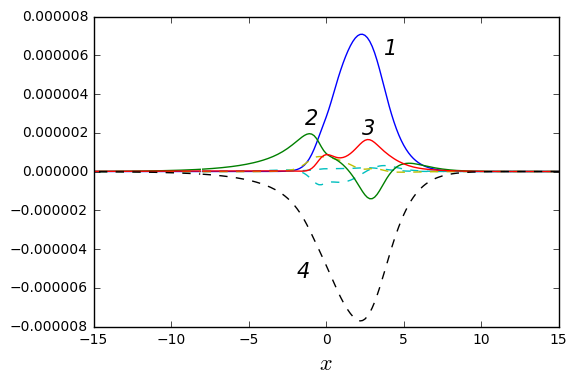
\includegraphics[width=0.6\linewidth]{ev_parts.png}}
\caption{Вклад в производство кинетической энергии движения $\V_V$, ассоциированного с продольными вихрями, со стороны: 1 --- $\v_n$; 2 --- $\V_{2D}$; 3 --- градиента давления; 4 --- вязких слагаемых. Другие слагаемые существенного вклада не дают.}
\label{ev_parts_pic}
\end{figure}

Аналогично, осреднение по $\theta$ уравнения \eqref{V3D_eq}, умноженного на поле скорости $\V_V$, ассоциированного с продольными вихрями, дает уравнение баланса кинетической энергии $E_V = \overline{\V_V^2/2}^\theta$:
\begin{equation}\label{EV_eq}
\pd{E_V}{t} = D_V^{2D} + D_V^{2D,S} + D_V^{S} + D_V^n - \overline{\V_V (\V_V \cdot \nabla) \V_V}^\theta - \overline{\V_V \nabla P_{3D}}^\theta + \nu \overline{\V_V \nabla^2 \V_V}^\theta,
\end{equation}
где слагаемые $D_V^{2D}$, $D_V^{2D,S}$, $D_V^S$, $D_V^n$ описывают влияние на поле скорости $\v_n$ компонент движения $\V_{2D}$, $\V_S$, $\V_n$, обусловленное нелинейным взаимодействие между ними. Значения $D_V^{2D}$, $D_V^{2D,S}$, $D_V^S$, $D_V^n$ вычисляются по формулам:
$$
D_V^{2D} = c \pd{E_V}{x} - (\V_{2D} \cdot \nabla) E_V - \overline{\V_V (\V_V \cdot \nabla)}^\theta \V_{2D},
$$
$$
D_V^{2D,S} = - \overline{\V_V (\V_S \cdot \nabla)}^\theta \V_{2D},
$$
$$
D_V^{S} = - \overline{\V_V (\V_S \cdot \nabla) \V_V}^\theta,
$$
$$
D_V^n = - \overline{\V_V (\v_n \cdot \nabla) \v_n}^{t,\theta}.
$$

Графики усредненных по сечению трубы слагаемых правой части уравнения \eqref{EV_eq} приведены на рисунке \ref{ev_parts_pic}. В соответствии с общими представлениями, наибольший вклад в производство продольных вихрей дает пульсационная составляющая движения. Её вклад в образование кинетической энергии $E_V$ выражает слагаемое $D_V^n$ (линия 1). Также существенный положительный вклад дает градиент давления, однако его интегральный вклад ниже почти в $5$ раз (линия 3). Слагаемое, выражающее вклад градиента давления в производство $E_V$, отлично от нуля, так как поле скорости $\V_V$ не соленоидальное. Также можно отметить влияние $\V_{2D}$, выраженное слагаемым $D_V^{2D}$ (линия 2). При $x > 0$ оно отрицательно, а при $x < 0$ --- положительно. Такое поведение соответствует тому, что продольная завихренность, формирующейся при положительных $x$, сносится вверх по течению вместе с основным потоком вблизи стенки за счет конвекции. Производство кинетической энергии $E_V$ перечисленными слагаемыми компенсируется вязким слагаемым (линия 4). Другие слагаемые в уравнении \eqref{EV_eq} существенного влияния не оказывают. 

\begin{figure}
\center{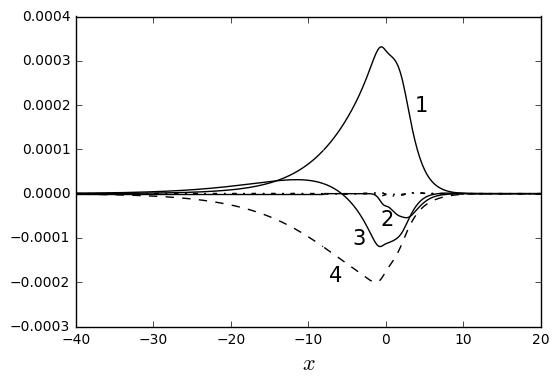
\includegraphics[width=0.6\linewidth]{es_parts.png}}
\caption{Вклад в кинетическую энергию движения $\V_S$, ассоциированного с полосами, со стороны: 1 --- $\V_V$ и $\V_{2D}$; 2 --- $\v_n$; 3 --- $\V_{2D}$; 4 --- вязких слагаемых. Другие слагаемые существенного вклада не дают.}
\label{es_parts_pic}
\end{figure}

Осреднение по переменной $\theta$ уравнения \eqref{V3D_eq}, умноженного на поле скорости $\V_S$,  ассоциированное с полосами, дает уравнение баланса кинетической энергии $E_S = \overline{\V_S^2/2}^\theta$:
\begin{equation}\label{ES_eq}
\pd{E_S}{t} = D_S^{2D} + D_S^{2D,V} + D_S^V + D_S^n - \overline{\V_S (\V_S \cdot \nabla) \V_S}^\theta - \overline{\V_S \nabla P_{3D}}^\theta + \nu \overline{\V_S \nabla^2 \V_S}^\theta.
\end{equation} 
Слагаемые $D_S^{2D}$, $D_S^{2D,V}$, $D_S^V$, $D_S^n$ вычисляются по формулам:
$$
D_S^{2D} = c \pd{E_S}{x} - (\V_{2D} \cdot \nabla) E_S - \overline{\V_S (\V_S \cdot \nabla)}^\theta \V_{2D},
$$
$$
D_S^{2D,V} = - \overline{\V_S (\V_V \cdot \nabla)}^\theta \V_{2D},
$$
$$
D_S^{V} = - \overline{\V_S (\V_V \cdot \nabla) \V_S}^\theta,
$$
$$
D_S^n = - \overline{\V_S (\v_n \cdot \nabla) \v_n}^{t,\theta}.
$$

Графики усредненных по сечению трубы слагаемых правой части уравнения \eqref{ES_eq} приведены на рисунке \ref{es_parts_pic}. В этом случае наибольший вклад дает слагаемое $D_S^{2D,V}$ (линия 1). Оно выражает совместное влияние на $\V_S$ со стороны компонент движения $\V_{2D}$ и $\V_V$ и в скалярных переменных имеет вид:
$$
D_S^{2D,V} =  - V_{x, S} V_{r, V} \pd{V_{x, 2D}}{r}.
$$
Доминирующая роль этого слагаемого согласуется с представлением о том, что продольные вихри формируются за счет <<лифт-ап>> эффекта. Нормальной к стенке трехмерная компонента скорости $V_{r,V} = V_{r,3D}$ перераспределяет продольный импульс двумерного основного течения $V_{x, 2D}$, образуя тем самым трехмерную составляющую продольной скорости $V_{x,3D} = V_{x,S}$. Пульсации оказывают небольшое отрицательное влияние на формирование полос (линия 2). Двумерное течение оказывает отрицательное влияние вблизи нуля, в то время, как в задней части порыва, при $x \sim -10$, его влияние оказывается положительным (линия 3). По-видимому, это связанно с конвективным переносом полос, формирующихся в передней части порыва, в его заднюю часть вблизи стенки, осуществляемое основным течением $\V_{2D}$. Получаемая составляющей движения $\V_S$ энергия компенсируется вязким слагаемым (линия 4). Другие слагаемые существенного влияния не оказывают. 

Полученные в разделе результаты подтверждают существующие представления о взаимодействии между компонентами движения модельного порыва. Также полученные результаты указывают на то, что все существенные взаимодействия между компонентами движения выделены и учтены. Данные о производстве кинетической энергии двумерной компоненты движения в разделе не приведены. За поддержание двумерного течения ответственен внешний перепад давления. Производимая внешним перепадом давления кинетическая энергия компенсируется вязкими слагаемыми. 



\section{Выводы по главе}

В главе представлены результаты численного исследования модельного порыва. Соответствующее модельному порыву решение уравнений Навье-Стокса является предельным состоянием решения, эволюционирующего на сепаратрисе, отделяющей в фазовом пространстве области притяжения решений, соответствующих ламинарному и турбулентному режимам течения. Предельное решение на сепаратрисе описывает локализованную в пространстве структуру, перемещающуюся вниз по потоку с постоянной скоростью. В сопутствующей системе отсчета при наложенных условиях симметрии оно оказывается периодическим по времени. Модельный порыв воспроизводит некоторые характерные особенности турбулентного порыва, а простота временного поведения позволяет выполнить его подробное исследование. Мы полагаем, что исследование модельного порыва может помочь приблизиться к пониманию турбулентного порыва.

При изучении модельного порыва установлены его основные характеристики, такие как скорость перемещения вдоль трубы и период изменения во времени. Составлено представление о внутренней структуре модельного порыва и выделены основные элементы цикла поддержания колебаний. Осреднение по времени в сопутствующей системе отсчета позволило разделить поле скорости модельного порыва на среднюю и пульсационную составляющие. Характерной особенностью среднего течения является наличие вытянутых вдоль трубы полос --- областей, скорость жидкости внутри которых существенно выше или ниже среднего значения. Полосы повышенной и пониженной скорости чередуются в угловом направлении. Показано, что пульсационная составляющая движения возникает в результате линейной неустойчивости среднего течения. Вероятным механизмом образования пульсаций является механизм типа Кельвина-Гельмгольца, так как пульсации возникают в области между полосами повышенной и пониженной скорости, где в среднем течении находятся точки перегиба, если рассматривать его как функцию угловой переменной. Изменение среднего течения вдоль оси $x$ существенного влияния на формирование пульсаций не оказывает. Показано, что полосы образуются за счет так называемого <<лифт-ап>> эффекта. В течении существуют стационарные продольные вихри, перемещающие жидкость в нормальной к основному потоку плоскости. Там, где медленная жидкость перемещается от стенки в основной поток, образуются полосы пониженной скорости. Между полосами пониженной скорости, где жидкость перемещается ближе к стенке, формируются полосы повышенной скорости. Формируясь в области небольшой протяженности, полосы вытягиваются вверх по потоку за счет конвекции. Полученные результаты позволяют сделать вывод о том, что поддержание стационарных продольных вихрей связано с наличием пульсаций. Такое представление подтверждается в следующей главе, посвященной механизму образования продольных вихрей.

Согласованность результатов, полученных на нескольких расчетных сетках, между собой и с результатами других авторов позволяет сделать вывод о том, что полученное предельное решение на сепаратрисе является решением уравнений Навье-Стокса и не зависит от выбора численного метода, которым оно было получено, и параметров расчета.

Выделенный в работе механизм поддержания модельного порыва согласуется с существующими представлениями о поддержании организованных структур в пристенных турбулентных течениях \cite{Hamilton1995, Waleffe1995, Waleffe1997, Jimenez1999, Schoppa2002}. Основным элементом организованных структур являются полосы повышенно и пониженной скорости, наблюдающиеся в буферном слое \cite{Kline1967, Smith1983}. Полосы в турбулентном течении перемещаются вдоль стенки и имеют ограниченное время жизни, но они достаточно хорошо различимы на фоне мелкомасштабных турбулентных пульсаций. Образование пульсаций в потоке связывают с неустойчивостью сдвиговых слоев, присутствующих в полосчатом течении. В работе \cite{Kim1971} сделан вывод о том, что производство турбулентных пульсаций в пристенных течениях практически полностью обусловлено периодически повторяющемся взрывообразным развитием неустойчивости на полосах пониженной скорости (<<bursting phenomenon>>). Считается, что полосы образуются за счет <<лифт-ап>> эффекта, но механизм образования продольных вихрей до сих пор не установлен. 



 

%[2] Kline, S. J., Reynolds, W. C., Schraub, F. A. & Runstadler, P. W. 1967 The structure of turbulent boundary layers. J. Fluid Mech. 30, 741–773.

%[19] Smith, C. R. & Metzler, S. P. 1983 The characteristics of low-speed streaks in the near-wall region of a turbulent boundary layer. J. Fluid Mech. 129, 27–54.

%[20] Kim, H. T., Kline, S. J. & Reynolds, W. C. 1971 The production of turbulence near a smooth wall in a turbulent boundary layers. J. Fluid Mech. 50, 133–160.

%[21] Hamilton, K., Kim, J. & Waleffe, F. 1995 Regeneration mechanisms of near-wall turbulence structures. J. Fluid Mech. 287, 317–348.
%[22] Jimenez, J. & Pinelli, A. 1999 The autonomous cycle of near wall turbulence. J. Fluid Mech. 389, 335–359.
%[23] Schoppa, W. & Hussain, F. 2002 Coherent structure generation in near-wall turbulence. J. Fluid Mech. 453, 57–108.
%[24] Waleffe, F. 1995 Hydrodynamic stability and turbulence: Beyond transients to a self-sustaining process. Stud. Appl. Maths 95, 319–343.
%[25] Waleffe, F. 1997 On a self-sustaining process in shear flows. Phys. Fluids 9, 883–900.













\chapter{Механизм поддержания продольных вихрей}


В предыдущей главе описан метод получения модельного порыва и его основные характеристики. Механизм самоподдержания модельного порыва оказывается связан с бегущей волной, которая может быть в нем выделена. Длина бегущей волны приблизительно равна 5 радиусам трубы $R$. Автором работы было обнаружено, что при условии $5R$ периодичности вдоль трубы метод поиска решения на сепаратрисе дает точную бегущую волну. Она повторяет основные особенности бегущей волны, наблюдаемой в модельном порыве, но является стационарной в сопутствующей системе отсчета. Простота поведения найденного решения позволила выделить нелинейный механизм взаимодействия пульсаций, ответственный за формирование продольных вихрей, и в строгом виде продемонстрировать ряд особенностей движения, обеспечивающих его работу. В этой главе представлены результаты исследования найденной бегущей волны и их обобщение на модельный порыв. 



\section{Характеристики возникающей на сепаратрисе бегущей волны}

Применение метода поиска решения на сепаратрисе, описанного в разделе \ref{edge_seq}, в расчетной области небольшой протяженности при $L_x = 5$, $\Re = 2200$ позволило получить решение типа нелинейной бегущей волны. Возникающая бегущая волна повторяет особенности бегущей волны, наблюдаемой в модельном порыве, однако, в отличии от нее, является точной в том смысле, что её поле скорости строго периодично вдоль трубы и во времени. В сопутствующей системе отсчета новое решение оказывается стационарным, что делает его более доступным для исследования. Фазовая скорость найденной бегущей волны равна $c_{tw} = 0.77$ (<<traveling wave>>), что соответствует скорости перемещения бегущей волны в модельном порыве. Возможно, найденная бегущая волна была получена также в \cite{Chantry2014}, где сообщается о том, что локализованное вдоль трубы решение, соответствующее модельному порыву, порождается некоторой бегущей волной вследствие потери ей симметрии. 

Как при исследовании модельного порыва, разделим поле скорости бегущей волны $\v_{tw}$ на стационарную $\V_{tw} = \overline{\v_{tw}}^{x}$ и пульсационную $\v_{n,tw} = \v_{tw} - \V_{tw}$ составляющие. В модельном порыве осреднение выполняется по времени в сопутствующей системе отсчета, в которой бегущая волна перемещается вниз по потоку. В случае точной бегущей волны такое осреднение эквивалентно осреднению вдоль трубы, что позволяет отказаться от переменной времени. Для того, чтобы представить средние характеристики бегущей волны на иллюстрации, достаточно привести их значение только в одном сечении трубы, так как они не зависят от $x$.

Продольная и поперечная компоненты среднего поля скорости бегущей волны $\V_{tw}$, изображены на рисунке \ref{pipetw_pic}(a,b). Оно повторяет среднее поле скорости модельного порыва в той области, где наблюдаются пульсации. На границах расчетной области, где быстрая жидкость проникает ближе к стенке, расположены полосы повышенной скорости, в центре расчетной области --- полоса пониженной скорости. Поперечное движение может быть ассоциировано с продольными вихрями. В расчетную область попадает пара таких вихрей, поддерживающих существование полос. Пульсационная составляющая, амплитуда которой изображена в на рисунке \ref{pipetw_pic}(с), также повторяет пульсации, наблюдаемые в модельном порыве (смотри рисунок \ref{puls_cs_pic}). Пульсации сосредоточены между полосами повышенной и пониженной скорости и в системе отсчета наблюдателя представляют собой волнообразное смещение области пониженной скорости в угловом направлении. Отметим, что движение жидких частиц может не совпадать с движением области пониженной скорости. Рисунок \ref{pipetw_pic}(d) позволяет сравнить мгновенное поле скорости пульсационной составляющей движения для бегущей волны $\v_{n,tw}$ и для модельного порыва~$\v_n$ (смотри рисунок \ref{puls_ls_pic}). На рисунках изображена продольная компонента скорости в сечении $\theta = 0$. 
 

\begin{figure}
\center{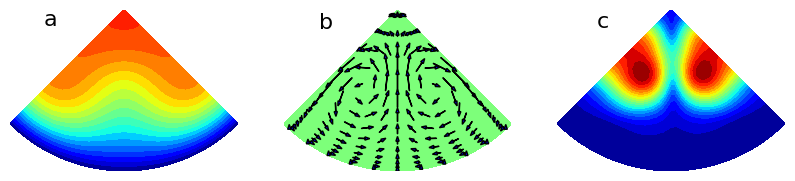
\includegraphics[width=0.9\linewidth]{pipetw_means.png}}
\center{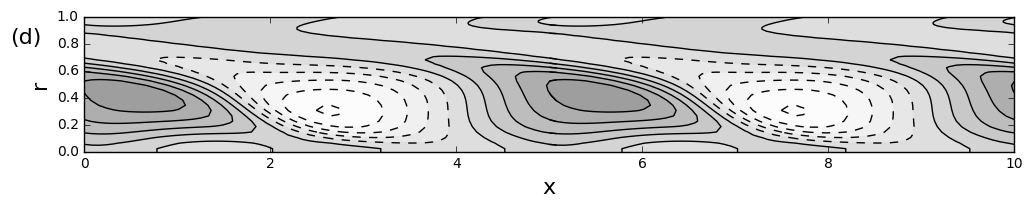
\includegraphics[width=0.9\linewidth]{pipetw_v1_ls.png}}
\caption{Поле скорости бегущей волны, возникающей на сепаратрисе: (a), (b) --- продольная и поперечная компоненты среднего течения $\V_{tw}$, (c) --- амплитуда пульсаций $\v_{n,tw}$, (d) --- продольная компонента пульсаций в сечении $\theta = 0$.}
\label{pipetw_pic}
\end{figure}

Хотя найденная бегущая волна повторяет качественные особенности модельного порыва, наблюдаются существенные количественные отличия. Для сравнения с модельным порывом, на рисунке \ref{pipetw_amp_pic} приведена амплитуда компонент движения бегущей волны, осредненная по времени и по сечению трубы. В отличии от модельного порыва, их значение не зависит от продольной координаты. По аналогии с модельным порывом, в среднем течении $\V_{tw}$ выделена двумерная компонента $\V_{2D,tw} = \overline{\V_{tw}}^\theta$. Трехмерная составляющая движения $\V_{3D,tw} = \V_{tw} - \V_{2D,tw}$ разделена на продольную $\V_{S,tw}$ и поперечную $\V_{V,tw}$, связанные с полосами и продольными вихрями, соответственно. Качественно соотношение между интенсивностью компонент движения сохраняется, однако в модельном порыве они достигают больших значений. Наибольшее отличие демонстрирует поперечное движение $\V_V$, для бегущей волны его значение более, чем в три раза ниже наибольшего значения, достигаемого в модельном порыве. Это может объясняться тем, что решение на сепаратрисе является равновесным. Равновесная интенсивность продольных вихрей в бегущей волне обусловлена необходимостью преодоления диссипирующего влияния вязкости. В модельном порыве необходима большая интенсивность вихрей для того, чтобы не только поддерживать, но и формировать полосы в попадающем внутрь порыва ламинарном течении. 


\begin{figure}
\center{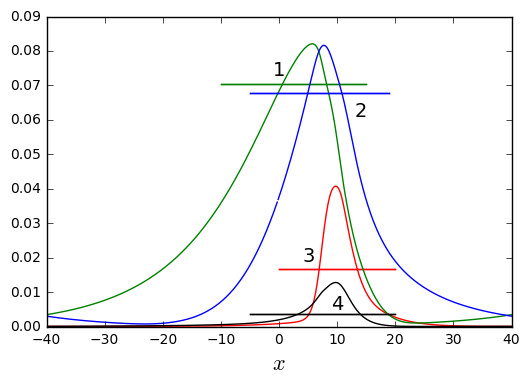
\includegraphics[width=0.5\linewidth]{pipetw_amp.png}}
\caption{Средняя по сечению трубы амплитуда компонент движения бегущей волны (горизонтальные линии) в сравнении с аналогичными величина для модельного порыва (функции переменной $x$): 1 --- движение $\V_S$, ассоциированное с полосами; 2 --- отклонение от течения Пуазейля двумерной компоненты движения $\V_{2D}$; 3 --- пульсационная составляющая движения $\v_n$; 4 --- движение $\V_V$, ассоциированное с продольными вихрями. График повторяет рисунок \ref{amp_pic}.}
\label{pipetw_amp_pic}
\end{figure}

Пульсационная составляющая движения бегущей волны $\v_{n,tw}$ возникает в результате линейной неустойчивости стационарного течения $\V_{tw}$. Наиболее быстро растущее собственное решение линеаризованного уравнения для возмущений \eqref{lin_eq} воспроизводит форму пульсационной составляющей движения и её фазовую скорость. Соответствующий инкремент нарастания $\lambda = 0.0085$. Для сравнения с пульсационной составляющей движения, поле скорости которой представлено на рисунке \ref{pipetw_pic}(c,d), на рисунке \ref{pipetw_lin_pic}(a,b) изображены амплитуда пульсаций, возникающих в линейной задаче, и их мгновенное поле скорости в продольном сечении. Решение линейной задачи имеет более простую форму. Так как среднее течение однородно вдоль трубы и стационарно, линейное решение имеет форму бегущей волны, поле скорости которой меняется по гармоническому закону вдоль трубы и во времени. Как и в случае с модельным порывом, возникающие в рамках линейной задачи пульсации имеют дополнительную симметрию отражения относительно сечения $\theta = \pi/4$, выражаемую уравнением \eqref{dop_sym_eq}. 


\begin{figure}
\center{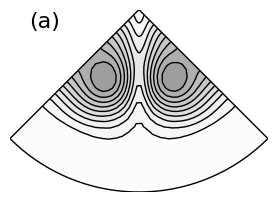
\includegraphics[width=0.3\linewidth]{pipetw_lin_amp.png} 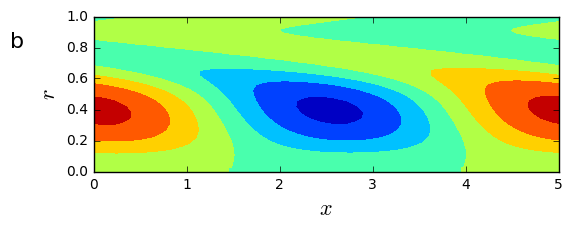
\includegraphics[width=0.6\linewidth]{pipetw_lin_ls.png}}
\caption{Наиболее быстрорастущее собственное возмущение, возникающее на среднем течении $\V_{tw}$: (a) --- амплитуда пульсаций, (b) --- продольная компонента скорости в сечении $\theta = 0$. }
\label{pipetw_lin_pic}
\end{figure}

%\lambda = - 0.0065


Возникающая на сепаратрисе бегущая волна, таким образом, воспроизводит основные элементы цикла самоподдержания модельного порыва, но имеет более простую форму. В сопутствующей системе отсчета её поле скорости оказывается стационарным. В потоке выделяются полосы повышенной и пониженной скорости. Области пониженной скорости имеют зигзагообразную форму. В системе отсчета наблюдателя движение представляет собой периодическое смещение области пониженной скорости в угловом направлении. С периодическим движением может быть ассоциирована пульсационная составляющая поля скорости. Было показано, что она возникает в результате линейной неустойчивости среднего течения, воспроизводящего полосчатый профиль скорости. Среднее течение в этом случае однородно вдоль трубы, что объясняет тот факт, что решение имеет форму бегущей волны. Также в потоке могут быть выделены стационарные продольные вихри, ответственные за образование полосчатого профиля скорости, также не меняющиеся вдоль трубы. Как будет показано далее, простота поведения бегущей волны позволяет выделить некоторые закономерности движения, справедливые также и для модельного порыва, и продемонстрировать их в строго виде. В частности, был выделен механизм нелинейного взаимодействия пульсаций, поддерживающий существование продольных вихрей. 


\section{Механизм образования продольных вихрей на примере точной бегущей волны}

Принято считать, что продольные вихри, ответственные за образование полос, возникают в результате некоторого нелинейного взаимодействия пульсаций, однако его детали не установлены. Прояснить процесс формирования продольных вихрей позволяет анализ уравнения, описывающего эволюцию продольной завихренности, полученного применением оператора Ротора к уравнению Навье-Стокса \eqref{NSeq_cf}:
\begin{equation}\label{ox_eq}
\pd{\omega_x}{t} - \nu\nabla^2 \omega_x =  -  (\v - \c_f, \nabla) \omega_x + (\om, \nabla) v_x
\end{equation}
Здесь $\om = (\omega_x, \omega_r, \omega_\theta) = \rot \v$ --- вектор завихренности, $\c_f$ --- скорость перемещения системы отсчета. Уравнение для стационарной составляющей продольной завихренности получается после осреднения \eqref{ox_eq} вдоль трубы:
\begin{equation}\label{OX_eq}
\pd{\Omega_x}{t} - \nu\nabla^2 \Omega_x = - (\V - \c_f, \nabla) \Omega_x + (\Om, \nabla) V_x - \overline{(\v', \nabla) \omega'_x}^x + \overline{ (\om', \nabla) v'_x }^x
\end{equation}
Здесь  $\Om=(\Omega_x, \Omega_r, \Omega_\theta)$ и $\om'=(\omega'_x, \omega'_r, \omega'_\theta)$ средняя и пульсационная составляющие вектора завихренности. Отметим, что в силу линейности оператора Ротора и осреднения $\Om = \rot \V$, $\om' = \rot \v'$, где $\V$ и $\v'$ --- средняя и пульсационная составляющие поля скорости $\v$. В правой части \eqref{OX_eq} первая пара членов описывает изменение продольной завихренности за счет конвективного переноса и деформации вихревых линий осредненного течения, а вторая пара выражает порождение средней завихренности пульсационным движением. При отсутствии пульсаций продольная завихренность постепенно исчезает под действием вязкости. В рассматриваемом течении система находится в равновесии и стационарная продольная завихренность во времени не меняется. Вязкие диссипация и диффузия компенсируются генерацией завихренности членами в правой части \eqref{OX_eq}.

Для выявления определяющих механизмов генерации средней продольной завихренности удобнее рассмотреть уравнение эволюции квадрата $\Omega_x$, получающееся домножением всех членов \eqref{OX_eq} на $2\Omega_x$. Положительный или отрицательный знак у полученных таким образом выражений в правой части уравнения показывает соответственно положительный или отрицательный вклад этого члена в изменение $\Omega_x^2$, а, следовательно, и в интенсивности поперечного движения. Распределение $\Omega_x^2$ по сечению трубы представлено на рис.~\ref{OXgen_pic}(a). В большей части сечения трубы средняя продольная завихренность близка к нулю. Область концентрации $\Omega_x$ расположена между полосами повышенной и пониженной скорости вблизи области максимальной амплитуды пульсаций.

\begin{figure}
\center{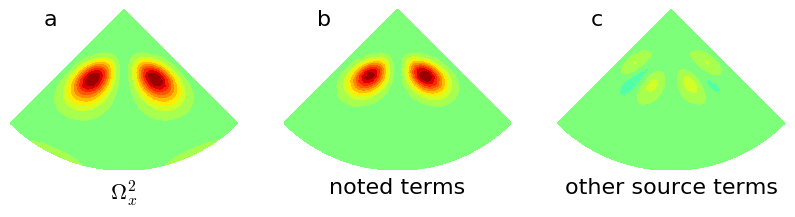
\includegraphics[width=1\linewidth]{pipetw_OXgen.png}}
\caption{Распределение по сечению трубы $\Omega_x^2$ --- (a), вклад в производство $\Omega_x^2$ слагаемых, соответствующих выделенным в \eqref{OXgen_terms} --- (b), вклад остальных слагаемых в правой части \eqref{OX_eq} --- (с). Сплошные линии соответствуют положительным значениям, прерывистые --- отрицательным.}
\label{OXgen_pic}
\end{figure}

При анализе уравнения \eqref{OX_eq} обнаружено, что два слагаемых в правой части вносят определяющий вклад в производство средней продольной завихренности. Они выделены в уравнении ниже:
\begin{equation}\label{OXgen_terms}
\pd{\Omega_x}{t} = - \overline{v'_x \frac{\d \omega'_x}{\d x}}^x + \overline{ \omega'_x \frac{\d v'_x}{\d x} }^x + ... 
\end{equation}
Соответствующее сумме \eqref{OXgen_terms}  распределение в уравнении для $\Omega_x^2$ представлено на рис.~\ref{OXgen_pic}(b), а вклад остальных слагаемых правой части \eqref{OX_eq} показан на рис.~\ref{OXgen_pic}(c). Распределение генерации $\Omega_x^2$ выделенными в \eqref{OXgen_terms} членами практически совпадает по форме с распределением $\Omega_x^2$, тогда как вклад остальных членов не имеет выраженного распределения и на порядок уступает по суммарному вкладу в генерацию $\Omega_x^2$. Таким образом, нет сомнения в том, что стационарные продольные вихри возникают в основном за счет действия выделенной в \eqref{OXgen_terms} пары слагаемых.

Отметим, что пульсации, соответствующие старшей собственной функции линейной задачи об устойчивости среднего стационарного течения, также демонстрируют приведенный выше механизм образования стационарных продольных вихрей. Важно, что это наблюдается только в том случае, когда при анализе устойчивости учитываются как продольная, так и поперечная составляющие среднего течения. Принято считать, что поперечное движение, определяя угловую неоднородность в распределении продольной скорости среднего течения, не может существенным образом влиять на свойства его устойчивости вследствие незначительности своей амплитуды. Поэтому при исследовании линейной устойчивости подобных течений, например, полосчатых структур в турбулентных потоках, наличие поперечного движения обычно не принимается во внимание. В нашем случае пренебрежение поперечным движением приводит к тому, что стационарное течение оказывается линейно устойчивым. Что еще более важно, наименее затухающее возмущение не воспроизводит при этом описанный механизм формирования продольных вихрей. Это связанно с тем, что форма пульсаций продольной завихренности $\omega'_x$ качественно меняется, хотя пульсации продольной скорости $v'_x$ сохраняют свою форму практически неизменной. Тем самым нарушается согласованность  $v'_x$ и $\omega'_x$, необходимая для обеспечения нужного вклада выражения \eqref{OXgen_terms} в производство продольной завихренности.

\begin{figure}
\center{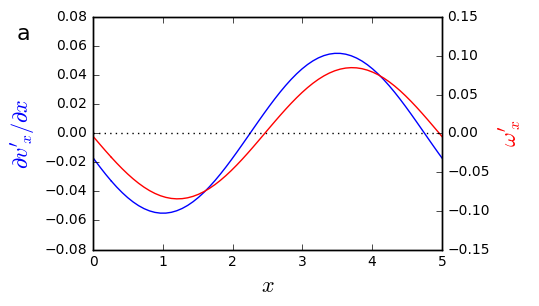
\includegraphics[width=0.5\linewidth]{pipetw_lin_cor.png}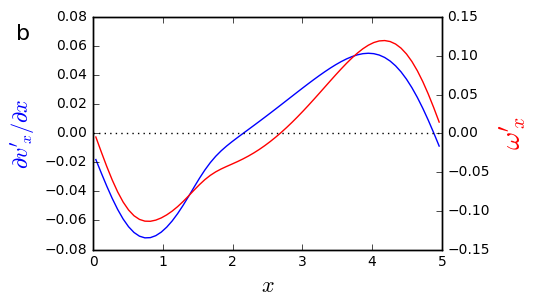
\includegraphics[width=0.5\linewidth]{pipetw_puls_cor.png}}
\caption{Значение $\d v_x' /\d x$ и $\omega_x'$ на прямой, проходящей через область, занятую положительным вихрем, $r = 0.5, \theta = \pi/8$: (a) --- для пульсаций, полученных в линейном приближении; (b) --- для пульсационной составляющей движения $\v_{tw} - \V_{tw}$. }
\label{OXgen_corr_pic}
\end{figure}


Каждое из двух слагаемых в \eqref{OXgen_terms} дает примерно половину общего вклада в производство средней продольной завихренности. Можно показать, что для пульсаций, полученных в рамках линеаризованной постановки, слагаемые \eqref{OXgen_terms} равны друг другу точно. Так как среднее поле скорости $\V_{tw}$ однородно вдоль трубы, возникающие на нем собственные возмущения меняются вдоль трубы по гармоническом закону. При фиксированных значениях $r$ и $\theta$ пусть  $v'_x = a \sin(\alpha x + \phi)$, $\omega_x' = b \sin(\alpha x + \psi)$, тогда:
\begin{equation} \label{OXgen_iterms_1}
 - v'_x \frac{\d \omega'_x}{\d x} = - \alpha a b \sin(\alpha x + \phi) \cos(\alpha x + \psi),
\end{equation}
\begin{equation} \label{OXgen_iterms_2}
\omega'_x \frac{\d v'_x}{\d x} =  \alpha a b \cos(\alpha x + \phi) \sin(\alpha x + \psi),
\end{equation}
\begin{equation} \label{OXgen_iterms_sum}
 - v'_x \frac{\d \omega'_x}{\d x} + \omega'_x \frac{\d v'_x}{\d x} = \alpha a b \sin(\psi - \phi).
\end{equation}
Осредненные вдоль трубы, слагаемые \eqref{OXgen_iterms_1}, \eqref{OXgen_iterms_2} в точности равны друг другу. Более того, сумма \eqref{OXgen_iterms_sum} не зависит от $x$, что, в частности, позволяет упустить знак осреднения вдоль трубы. Эффективность производства  $\Omega_x$ определяется разностью фаз $\psi - \phi$. В области положительного вихря, при $a,b > 0$, наибольшую эффективность как первому, так и второму слагаемому обеспечивает значение $\psi - \phi = \pi/2$. В этом случае $\d v'_x/\d x$ и $\omega'_x$ положительно коррелированы в то время, как $\d v'_x/\d x$ и $\omega'_x$ --- отрицательно. В области отрицательного вихря ситуация меняется на противоположную. Расчет соответствующих коэффициентов корреляции показывает, что они близки к $\pm1$ в соответствующих областях. В качестве подтверждения на рисунке \ref{OXgen_corr_pic}(a) представлены значения $\d v'_x/\d x$ и $\omega'_x$ на прямой, проходящей через область, занятую положительным вихрем, $r = 0.5, \theta = \pi/8$. Фазы выделенных компонент движения практически совпадают. Указанное свойство сохраняется также для пульсационной составляющей движения $\v_{tw} - \V_{tw}$, для которой аналогичные величины изображены на рисунке \ref{OXgen_corr_pic}(b). Объяснить наблюдаемую согласованность фаз позволяет механизм образования пульсаций продольной завихренности, выделенный при исследовании бегущей волны, представленный в следующем разделе. Отметим, что, так как решения являются бегущими волнами, изображенное на рисунке \ref{OXgen_corr_pic} картина течения сохраняется неизменной во времени. 


\section{Механизм образования пульсаций продольной завихренности на примере точной бегущей волны}

Для выявления механизма формирования выделенной связи между пульсациями продольных компонент скорости и завихренности рассмотрим уравнение эволюции $\omega'_x$, получающееся вычитанием \eqref{OX_eq} из \eqref{ox_eq}:
\begin{multline}\label{ox1_eq}
\pd{\omega'_x}{t} - \nu \nabla^2 \omega'_x = - (\V - \c, \nabla) \omega'_x - (\v', \nabla) \Omega_x
+(\Om, \nabla) v'_x + (\om', \nabla) V_x -\\- (\v', \nabla) \omega'_x  + (\om', \nabla) v'_x  + \overline{(\v', \nabla) \omega'_x)}^x  - \overline{(\om', \nabla)}^x
\end{multline}
Работать удобнее с уравнением, описывающим изменение среднего квадрата пульсаций продольной завихренности $\overline{\omega'^2_x}$, получающимся умножением на $2\omega'_x$ каждого из слагаемых в \eqref{ox1_eq} и последующим осреднением вдоль трубы. Слагаемые в этом уравнении не зависят от времени и продольной координаты, сумма слагаемых в правой части балансируется вязким членом в левой части. Как и в предыдущем случае, среди всех слагаемых правой части удается выделить существенные, ответственные за возникновение пульсаций $\omega'_x$.


Распределение $\overline{\omega'_x \omega'_x}^x$ по сечению трубы изображено на рис.~\ref{ox1gen_pic}(a). Основные пульсации $\omega'_x$ наблюдаются в центре расчетной области около оси трубы. На месте расположения продольных вихрей также присутствуют пульсации $\omega'_x$, но меньшей интенсивности. В остальной части трубы их амплитуда близка к нулю. Обнаружено, что за генерацию пульсаций $\omega'_x$ в центральной части трубы и на месте продольных вихрей отвечают два разных механизма. Первый дает пульсации большей амплитуды, однако, за возникновение стационарных продольных вихрей ответственны пульсации, производимые вторым механизмом, так как именно они оказываются согласованными с пульсациями $v'_x$ нужным образом.


\begin{figure}
\center{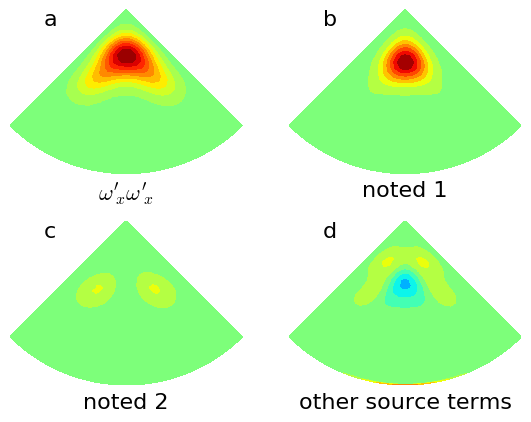
\includegraphics[width=0.66\linewidth]{pipetw_ox1gen.png}}
\caption{Распределение среднего квадрата пульсаций продольной завихренности --- а, вклад в производство $\overline{\omega'_x \omega'_x }^x$ слагаемых \eqref{ox1gen_add_terms} --- (b), слагаемого \eqref{ox1gen_main_terms} --- (c) и суммы остальных слагаемых правой части \eqref{ox1_eq} --- (d).}
\label{ox1gen_pic}
\end{figure}


Первый механизм формирования $\omega'_x$ связан с наличием нормальных к стенке вихрей в пульсационной составляющей движения. Можно провести аналогию между неустойчивостью, возникающей на полосе замедления, и неустойчивостью в следе за телом. Пульсационная составляющая движения напоминает дорожку Кармана. В ней можно выделить последовательность нормальных к стенке вихрей чередующегося знака, двигающихся вниз по полосе пониженной скорости. Им соответствуют области повышенной амплитуды пульсаций радиальной завихренности $\omega'_r$. На рисунке \ref{pipetw_or1_pic} изображена $\omega'_r$ в сечении $r = 0.5$, нормальном к выделенной компоненте завихренности. Приведенные на \ref{pipetw_or1_pic}(a) значения посчитаны по пульсациям, полученным в рамках линеаризованной задачи. Аналогичные значения для пульсационной составляющей движения $\v_{tw} - \V_{tw}$ представлены на рисунке \ref{pipetw_or1_pic}(b). Амплитуда пульсаций продольной завихренности оказывается на порядок ниже амплитуды пульсаций радиальной, угловая завихренность в центральной части трубы также равна нулю в силу симметрии. Таким образом, в центральной части трубы поле завихренности представлено в первую очередь радиальной компонентой и соответствует нормальным к стенке вихрям.

Пульсации продольной завихренности $\omega'_x$ возникают вследствие поворота нормальных к стенке вихрей, происходящего в присутствии градиента продольной скорости $\d V_x/ \d r$, возникающего между полосой замедления и стенкой трубы. Кроме того, наличие радиального градиента $\d V_x/ \d r$ связано с наличием угловой завихренности $\Omega_\theta = \d V_r / \d x - \d V_x / \d r$. Радиальная пульсационная завихренность $\omega'_r = \d v'_x / r \d \theta - \d v'_\theta / \d x$ за счет первого из слагаемых поворачивает стационарные угловые вихри так, что те также приобретают пульсационную продольную составляющую. В уравнении \eqref{ox1_eq} за описанный механизм отвечают слагаемые:
\begin{equation}\label{ox1gen_add_terms}
\frac{\d \omega'_x}{\d t} = \omega'_r \frac {\d V_x}{\d r} + \frac{\Omega_\theta}{r} \frac{\d v'_x}{\d \theta} + ...
\end{equation}
Несмотря на то, что выделенные в \eqref{ox1gen_add_terms} слагаемые имеют противоположные знаки и в значительной степени компенсируют друг друга при сложении, их вклад в производство $\omega'_x$ значителен (смотри рисунок~\ref{ox1gen_pic}(b)). Они определяют форму пульсаций $\omega'_x$ в области между полосой замедления и осью трубы, где пульсации $\omega'_x$ достигают наибольшего значения. Эти пульсации, однако, практически не участвуют в образовании стационарной составляющей продольной завихренности. Это объясняется тем, что колебания $\omega'_x$, рождающиеся в результате описанного механизма, близки по фазе к колебаниям $v'_x$, так что сомножители каждого из слагаемых в выражении \eqref{OXgen_terms} оказываются в противофазе и при осреднении дают близкие к нулю значения.

\begin{figure}
\center{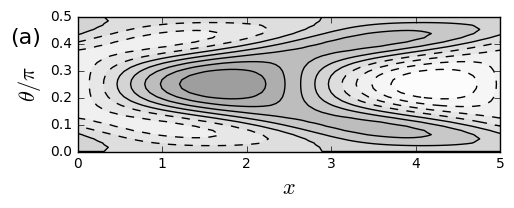
\includegraphics[width=0.45\linewidth]{pipetw_or1_lin.png} 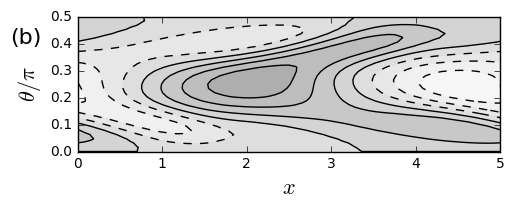
\includegraphics[width=0.45\linewidth]{pipetw_or1.png}}
\caption{Нормальная к стенке компонента завихренности $\omega_r'$ в сечении $r = 0.5$: (а) --- для пульсаций, полученных в рамках линейного приближения; (b) --- для пульсационной составляющей движения $\v_{tw} - \V_{tw}$. }
\label{pipetw_or1_pic}
\end{figure}

Второй механизм образования пульсаций продольной завихренности $\omega'_x$ связан с перераспределением уже существующей стационарной продольной завихренности $\Omega_x$ за счет пульсационной составляющей продольной скорости $v'_x$ (эффект сжатия/растяжения вихревых линий). В уравнении \eqref{ox1_eq} за описываемый механизм отвечает слагаемое
\begin{equation}\label{ox1gen_main_terms}
\frac{\d \omega'_x}{\d t} = \Omega_x \frac {\d v'_x}{\d x} + ...
\end{equation}
Выделенное в \eqref{ox1gen_main_terms} слагаемое стремится произвести пульсации $\omega'_x$, пропорциональные $\d v'_x / \d x$, что обеспечивает наибольшую эффективность образования $\Omega_x$ посредством их нелинейного взаимодействия. Важно, что коэффициентом пропорциональности в \eqref{ox1gen_main_terms} выступает значение средней продольной завихренности, таким образом, механизм включается именно в областях концентрации $\Omega_x$. При этом производимые пульсации $\omega'_x$ положительно пропорциональны пульсациям  $\d v'_x / \d x$ при $\Omega_x>0$ и отрицательно пропорциональны при $\Omega_x<0$, что обеспечивает максимально возможную эффективность производства средней продольной завихренности нужного знака посредством второго из слагаемых выражения \eqref{OXgen_terms}. Очевидно, что пульсации $-v'_x$ и $\d \omega'_x / \d x$ в этом случае также согласованы нужным образом, так что первое слагаемое \eqref{OXgen_terms} близко по значению ко второму.

На рисунке~\ref{ox1gen_pic}(c) приведен вклад выделенного в \eqref{ox1gen_main_terms} слагаемого в производство $\overline{\omega'_x \omega'_x}^x$. Это слагаемое определяет форму пульсаций в области существования продольных вихрей между полосами повышенной и пониженной скорости. Суммарный вклад других слагаемых правой части \eqref{ox1_eq}, не попавших на рис.~\ref{ox1gen_pic}(b,c), изображен на рис.~\ref{ox1gen_pic}(d). Эти слагаемые не имеют существенного значения в процессе генерации $\omega'_x$, их суммарный вклад не превышает нескольких процентов. 

Описанный механизм генерации пульсаций продольной завихренности проявляется в области, где фазовая скорость волны, соответствующей пульсационной составляющей течения, близка по значению к локальной продольной скорости среднего течения. На удалении от точки генерации пульсаций, где фазовая скорость волны существенно отличается от средней скорости, выделенный в \eqref{ox1gen_main_terms} механизм генерации $\omega'_x$ практически не работает. Это объясняется тем, что в системе отсчета, связанной с волной, образующаяся посредством механизма \eqref{ox1gen_main_terms} $\omega'_x$ сносится вдоль трубы средним течением. При этом теряется согласованность фаз между $\d v'_x / \d x$ и $\omega'_x$, что делает её рост невозможным. 


\section{Обобщение полученных при изучении точной бегущей волны результатов на модельный порыв}


\begin{figure}
\center{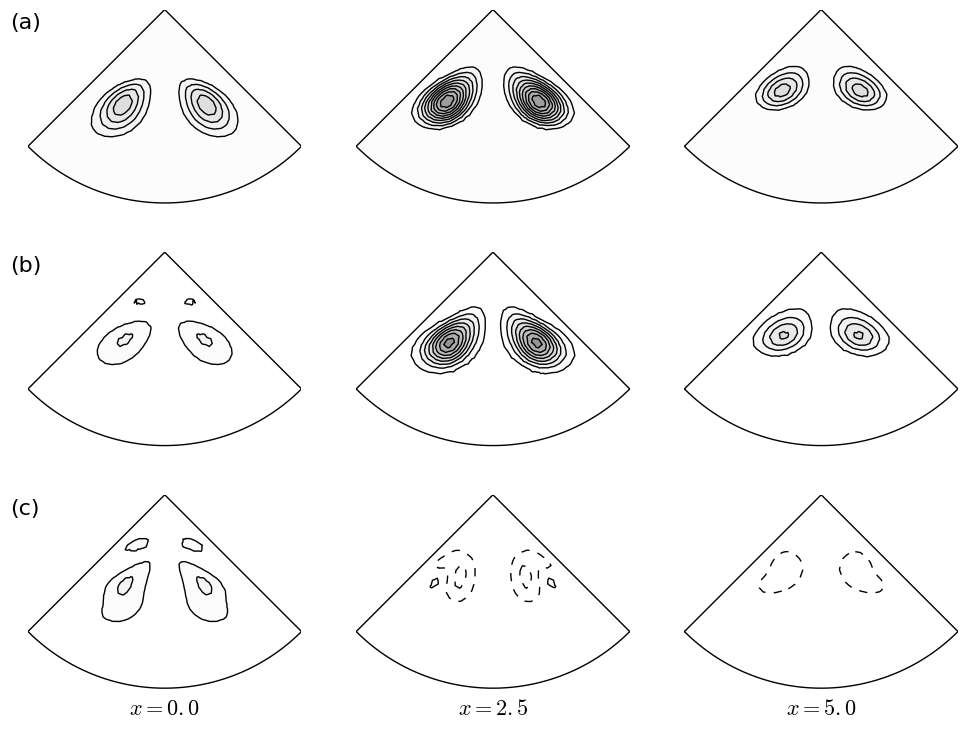
\includegraphics[width=0.9\linewidth]{puff_OXgen.png}}
\caption{В нескольких сечения трубы изображена $\Omega_x^2$ --- в строке (а), а также вклад в образование $\Omega_x^2$ со стороны слагаемых \eqref{OXgen_term} и других слагемых в правой чсти уравнения \eqref{tOX_eq}.}
\label{puff_OXgen_pic}
\end{figure}


Выделенный при изучении бегущей волны, возникающей на сепаратрисе в непротяженной расчетной области, механизм образования продольных вихрей может быть обобщен на модельный порыв. В этом случае осреднение выполняется по времени в системе отсчета, связанной с порывом. Для точной бегущей волны такое осреднение и осреднение вдоль трубы эквивалентны друг другу, так как в системе отсчета порыва она движется. 

Разделим поле завихренности $\om = \rot \v$ на среднюю $\Om = (\Omega_x, \Omega_r, \Omega_\theta) = \overline{\om}^t$ и пульсационную $\om' = (\omega'_x, \omega'_r, \omega'_\theta) = \om - \Om$ составляющие. Как и в случае бегущей волны, поле стационарной продольной завихренности $\Omega_x$ модельного порыва воспроизводит пару продольных вихрей, расположенных по бокам от полосы пониженной скорости. 



Осреднение \eqref{ox_eq} по времени дает уравнение баланса $\Omega_x$: 
\begin{equation} \label{tOX_eq}
\pd{\Omega_x}{t} - \nu\nabla^2 \Omega_x = - (\V - \c_f, \nabla) \Omega_x + (\Om, \nabla) V_x - \overline{(\v', \nabla) \omega'_x}^t + \overline{ (\om', \nabla) v'_x }^t.
\end{equation}

\begin{figure}
\center{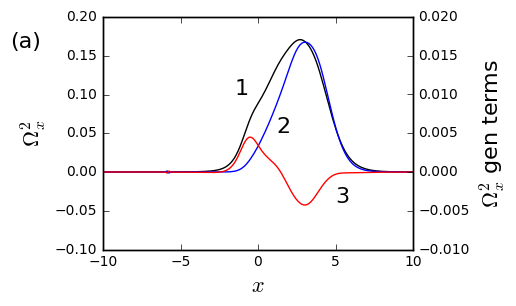
\includegraphics[width=0.5\linewidth]{xline_OXgen.png}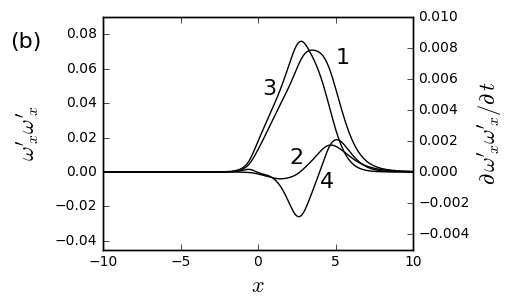
\includegraphics[width=0.5\linewidth]{xline_ox1gen.png}}
\caption{На прямой, проходящей через область, занятую продольным вихрем, при $r = 0.5, \theta = \pi/8$, изображены: (a) --- Квадрат стационарной продольной завихренности (кривая 1) и вклад в его производство со стороны \eqref{OXgen_term} (кривая  2) и других слагаемых в правой части уравнения \eqref{tOX_eq} (кривая  3); (b) --- средний квадрат пульсаций продольной завихренности $\overline{\omega'_x \omega'_x}^t$ (кривая 1) и вклад в его производство со стороны \eqref{ox1gen_term1} (кривая  2), \eqref{ox1gen_term2} (кривая  3) и других слагаемых в правой части уравнения \eqref{tox1gen_eq} (кривая  4).}
\label{xline_oxgen_pic}
\end{figure}


\begin{figure}
\center{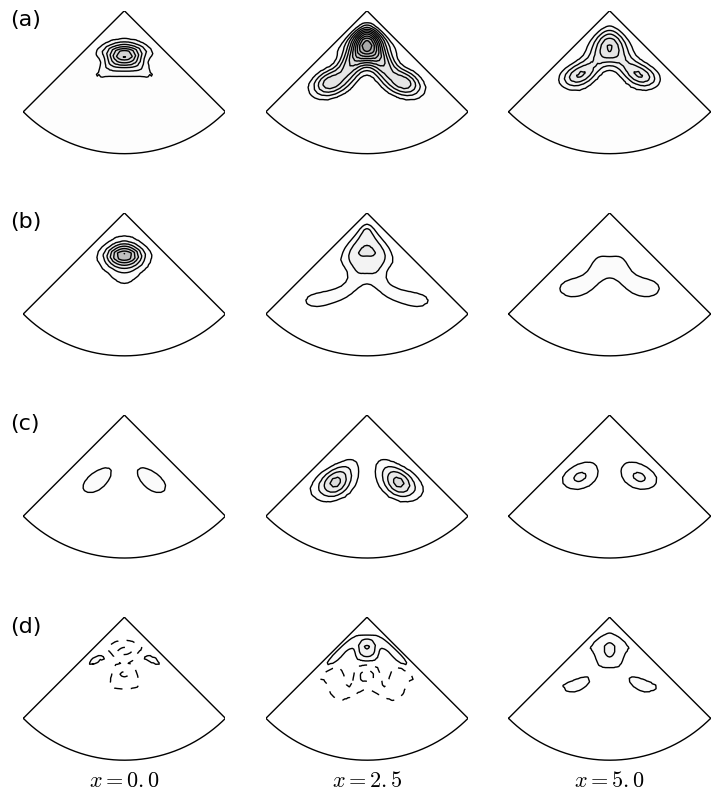
\includegraphics[width=0.9\linewidth]{puff_ox1gen.png}}
\caption{В нескольких сечения трубы изображены: ряд (a) --- интенсивность пульсаций продольной завихренности $\overline{\omega'_x \omega'_x}^t$, ряд (b) --- вклад в образование $\overline{\omega'_x \omega'_x}^t$ со стороны слагаемых \eqref{ox1gen_term1}, ряд (c) --- со стороны слагаемого \eqref{ox1gen_term2}, ряд (d) --- со стороны других других слагаемых в правой части \eqref{tox1gen_eq}. Каждый столбец соответствует одному сечению трубы. }
\label{puff_ox1gen_pic}
\end{figure}

\section{Необходимость учета поперечной компоненты стационарного течения для адекватного воспроизведения формы пульсаций}

Отметим, что пульсации, соответствующие старшей собственной функции линейной задачи об устойчивости среднего стационарного течения, также демонстрируют приведенный выше механизм образования стационарных продольных вихрей. Важно, что это наблюдается только в том случае, когда при анализе устойчивости учитываются как продольная, так и поперечная составляющие среднего течения. Принято считать, что поперечное движение, определяя угловую неоднородность в распределении продольной скорости среднего течения, не может существенным образом влиять на свойства его устойчивости вследствие незначительности своей амплитуды. Поэтому при исследовании линейной устойчивости подобных течений, например, полосчатых структур в турбулентных потоках, наличие поперечного движения обычно не принимается во внимание. В нашем случае пренебрежение поперечным движением приводит к тому, что стационарное течение оказывается линейно устойчивым. Что еще более важно, наименее затухающее возмущение не воспроизводит при этом описанный механизм формирования продольных вихрей. Это связанно с тем, что форма пульсаций продольной завихренности $\omega'_x$ качественно меняется, хотя пульсации продольной скорости $v'_x$ сохраняют свою форму практически неизменной. Тем самым нарушается согласованность  $v'_x$ и $\omega'_x$, необходимая для обеспечения нужного вклада выражения \eqref{OXgen_terms} в производство продольной завихренности.


Описанный механизм генерации пульсаций продольной завихренности объясняет необходимость учета поперечного движения при исследовании устойчивости стационарного течения. Пренебрежение связанной с поперечным движением $\Omega_x$ делает невозможным генерацию $\omega'_x$ в форме, необходимой для сохранения поперечного движения, а следовательно и всего процесса самоподдержания пульсаций.


\section{Выводы по главе}

ы


\chapter{Верификация полученных результатов}


В предыдущих главах, исследуя модельный порыв, удалось получить некоторые представления о его структуре и механизме самоподдержания. В настоящей главе поднимается вопрос об общности полученных результатов. Наличие пристенных полос повышенной и пониженной скорости является характерной особенности многих инвариантных решений уравнений Навье-Стокса \cite{Kawahara2012} и пристенной турбулентности непосредственно \cite{Kline1967, Smith1983, Schoppa2002}. Это обстоятельство позволяет надеяться, что выделенные при исследовании модельного порыва особенности движения, могут быть в некоторой степени обобщены и на эти случаи. Выполнить строгое исследование турбулентного течения сегодня не представляется возможным, однако полученные результаты могут быть проверены на других инвариантны решения. Продлевая решение, соответствующее модельному порыву, по числу Рейнольдса \cite{Sanchez2004, Viswanath2007, Dijkstra2014}, удалось получить новое локализованное в пространстве условно периодическое по времени решение, характеристики которого оказываются ближе к характеристикам турбулентного течения. Также удалось получить несколько различных бегущих волн в круглой трубе и плоском канале Пуазейля. В настоящей главе представлены методы получения инвариантных решений и результаты их исследования. 


\section{Семейство условно периодических по времени решений поставленной задачи}

Решение поставленной задачи $\v_p(x,r,\theta,t)$ является периодическим по времени с периодом $T$, если оно удовлетворяет условию:
\begin{equation} \label{tper_eq}
\v_p(x,r,\theta,t) = \v_p(x - c_p T, r, \theta, t + T).
\end{equation}
Здесь $c_p$ --- скорость перемещения периодического решения вдоль трубы. В конечно-разностной постановке условие \eqref{tper_eq} может быть сформулировано иначе:
\begin{equation}\label{P_eq}
\phi(\v_p, T, c_p, \Re) - \v_p = 0.
\end{equation}
Здесь функция $\phi(\v, t, c, \Re)$ возвращает поле скорости, возникающее в результате эволюции поля скорости $\v$ в течении времени $t$ при числе Рейнольдса $\Re$ в системе отсчета, перемещающейся со скоростью $c$. В число параметров функции $\phi$ могут входить также и другие величины, такие как длина периода вдоль трубы $L_x$ или длина периода в угловом направлении $L_{\theta} = 2\pi/n$ (в некоторых случаях $n$ может быть действительным). С практической точки зрения, вычисление функции $\phi$ требует численного интегрирования поля скорости $\v$ по времени. 

Периодические решения обладают двумя непрерывными симметриями: решение остается решение при его смещении вдоль трубы на произвольное расстояние и при смещении по времени на произвольную величину. Для того, чтобы каждому решению \eqref{P_eq} соответствовало только одно поле скорости $\v_p$, необходимо дополнить систему двумя уравнениями, исключающими возможность указанных смещений, имеющими вид:
\begin{equation}\label{Pplus_eq}
r_{1,2}(\v_p) = 0.
\end{equation}
В этом случае, если поле скорости однозначно задается $N$ переменными, то количество уравнений в системе равно $N+2$. Для того, чтобы число неизвестных в системе совпадало с числом уравнений, необходимо вместе с полем скорости $\v_p$ положить неизвестными два параметра системы. В случае, если решение ищется при фиксированном значении $\Re$ на заданной сетке, это будут $T$ и $c_p$. Их значение однозначно определяется вместе с полем скорости.

Система \eqref{P_eq}, \eqref{Pplus_eq} может быть представлена в виде:
\begin{equation}\label{F_eq}
F(\x) = 0, 
\end{equation}
где вектор $\x = (\v_p, T, c_p, \Re)$ объединяет все переменные. Рассмотрим её полный дифференциал
\begin{equation}\label{dF_eq}
dF = \pd{F}{\x}d\x.
\end{equation}
В случае, если фиксированы все параметры кроме трех, например, $T$, $c_p$ и $\Re$, Якобиан ${\d F}/{\d \x}$ оказывается прямоугольной матрицей, содержащей $(N+2)$ строк и $(N+3)$ столбцов. Система \eqref{dF_eq} недоопределена. В этом случае в окрестности каждого решения существует направление $d\x^*$, для которого $dF = 0$, при движении вдоль которого решение остается решением, так как значение $F$ сохраняется равным нулю. Тогда решения в пространстве трех параметров принадлежат некоторой кривой, задаваемой одним параметром $s$, полученной интегрирование вдоль направления $d\x^*$:
$$
\x_p = \Gamma(s).
$$ 
Аналогично, в пространстве четырех параметров решения принадлежат двухпараметрическому семейству, и т.д. 

Решение, соответствующее модельному порыву, принадлежит семейству условно периодических по времени решений. Естественно считать геометрию расчетной области постоянной. Тогда неизвестными остаются три параметра $\Re$, $T$ и $c_p$. В пространстве трех параметров решение принадлежит однопараметрическому множеству. В соответствии с \cite{Avila2013}, продлевая решение в сторону уменьшения числа Рейнольдса, удается достичь точки бифуркации, в которой рождается две ветви решения (кривая, которой принадлежат решения, совершает разворот так, что при меньших $\Re$ решение не существует). Метод продления решения по параметру представлен в следующем разделе. Исходное решение принадлежит нижней ветви. Верхняя ветвь решения характеризуется большей амплитудой пульсаций, скорость перемещения вдоль трубы соответствующего решению порыва оказывается ближе к скорости перемещения турбулентного порыва. Если решения с нижней ветви принадлежат сепаратрисе, верхняя ветвь находится внутри области притяжения турбулентного режима течения и может участвовать в организации турбулентного аттрактора. Мы считаем, что результаты, полученные при изучении решения с верхней ветви, имеют б\'{о}льшую ценность, так как его характеристики ближе к характеристика турбулентного течения. 

Отметим, что вместо условия периодичности по времени \eqref{tper_eq} может быть применено условие отражения относительно плоскости $\theta = 0$ со сдвигом на половину периода по времени $T/2$, которое выполнено для модельного порыва. Условие имеет вид:
\begin{multline}\label{shift_eq}
(v_{x,p}, v_{r,p}, - v_{\theta,p})(x,r,\pi/4 + \theta,t) = \\ =(v_{x,p}, v_{r,p}, v_{\theta,p})(x - c_p T/2,r,\pi/4 - \theta,t+T/2).
\end{multline}
В этом случае \eqref{P_eq} уступит место условию:
\begin{equation}\label{P2_eq}
(v_{x,p}, v_{r,p}, - v_{\theta,p})(x,r,\pi/4 - \theta) = \phi(\v_p, T/2, c_p, \Re)(x,r,\pi/4 + \theta).
\end{equation}
Его вычисление требует вдвое меньше времени, что может быть существенно при проведении численного исследования. При решении исходной системы \eqref{P_eq} существует возможность потери симметрии \eqref{shift_eq} в процессе продления решения, что исключено при решении системы \eqref{P2_eq}.


\section{Метод Ньютона-Крылова для поиска условно периодических по времени решений} \label{Newton_seq}

Численно найти условно периодические по времени решения, удовлетворяющие нелинейной системе \eqref{F_eq}, позволяет метод Ньютона, обобщенный на многомерный случай. Метод Ньютона итерационный и на каждом шаге уточняет существующее приближение к решению. Пусть $x_m$ --- приближение к решению на шаге $m$, $x^*$ --- точное решение. Разложение выражения $F(x^*)$ в ряд около точки $x_m$ имеет вид:
\begin{equation}
F(x^*) = F(x_m) + \pd{F}{x}\bigg|_{x=x_m} \Delta x_m^* + O(\Delta x_m^{*2}), 
\end{equation}
где $\Delta x_m^* = x^* - x_m$. Пренебрегая малыми второго порядка, учитывая, что $F(x^*) = 0$, получим линейную систему на поправку к решению $\Delta x_m$:
\begin{equation}\label{Newton_eq}
\pd{F}{x}\bigg|_{x = x_m} \Delta x_m = - F(x_m). 
\end{equation}
Основной задачей при применении метода Ньютона является решение системы \eqref{Newton_eq} и нахождение $\Delta x_m$. Выполнение шага метода Ньютона завешается вычисление нового приближения к решению: 
\begin{equation} \label{end_NK_eq}
x_{m+1} = x_m + \Delta x_m. 
\end{equation}

В случае численного решения задач гидродинамики размерность системы \eqref{Newton_eq} оказывается достаточно большой (в нашем случае $N \sim 10^6$), её решение требует значительных вычислительных ресурсов. Еще более сложной задачей является формирование матрицы Якоби $J(x) = \partial F / \partial x $ в явном виде. При поиске периодических решений привести аналитическое выражение для Якобиана не представляет возможным. Для формирования матрицы Якоби пользуются тем фактом, что её произведение с произвольным вектором единичной длины $l$ равно производной исходно функции $F$ вдоль этого направления:
\begin{equation} \label{Jl_eq}
\pd{F}{x} l = \pd{F}{l}. 
\end{equation}
Значение производной функции $F$ может быть получено численно, как конечная разность, по формуле:
\begin{equation}\label{fd_eq}
\pd{F}{l} \approx \frac{F(x + \varepsilon l) - F(x)}{\varepsilon}.
\end{equation}
В расчетах значение $\varepsilon$ рекомендуется выбирать близким к $10^{-7}$ \cite{Viswanath2007}. Формирование матрицы Якоби сводится к вычислению производной функции $F$ вдоль каждого из базисных направлений, число которых равно числу неизвестных. Вычисление производной $F$ вдоль одного направления требует вычисления функции $F$ в новой точке. Таким образом, формирование матрицы Якоби сводится к $O(N)$ вызовам функции интегрирования по времени, что является крайне трудоемкой задачей. 


Решить линейную систему \eqref{Newton_eq} позволяют итерационные методы, основанные на подпространствах Крылова \cite{Sanchez2004}. В этом случае обращение к матрице Якоби происходит только в форме её умножения на вектор, что в соответствии с \eqref{fd_eq} сводится к вычислению конечно-разностной производной функции $F$ вдоль направления, задаваемого этим вектором. При решении системы вида
\begin{equation}\label{Ax_eq}
Ax = b
\end{equation}
подпространство Крылова $K_i$ представляет собой линейную оболочку $i$ векторов:
\begin{equation}\label{Ki_eq}
K_i = L(b, Ab, A^2b, \dots, A^{i-1}b).
\end{equation}
Имея базис подпространства $K_i$, для того, чтобы построить базис в подпространстве $K_{i+1}$, необходимо выполнить только одно умножение матрицы $A$ на уже известный вектор $A^{i-1}b$. При решении системы \eqref{Ax_eq} приближение к решению ищется в базисе подпространства Крылова. Крыловские методы оказываются эффективны при поиске инвариантных решений с небольшим числом неустойчивых направлений (решение на сепаратрисе имеет одно неустойчивое направление \cite{Avila2013}). Для уточнения решения на порядок требуется только несколько десятков базисных векторов и их число не зависит от $N$. Метод Ньютона, в котором для решение линейной системы \eqref{Newton_eq} применяются методы Крыловского типа, называется также методом Ньютона-Крылова \cite{Sanchez2004}. 

Подпространство Крылова может быть построено только в случае, если в системе \eqref{Ax_eq} матрица $A$ --- квадратная. Число неизвестных в исходной системе \eqref{F_eq} должно быть равно числу уравнений. Этого можно добиться, фиксировав значения всех параметров, кроме двух, например, $T$ и $c_p$. Либо, если определению подлежит большее число параметров, можно дополнить систему \eqref{F_eq} уравнениями, определяющими связь между ними. 

В работе был реализован основанный на подпространствах Крылова метод минимизации невязки ("MINRES" --- "Minimum residual method")\cite{EEbook}. Суть метода состоит в том, что на $i$-ой итерации в подпространстве $K_i$ ищется приближение к решению $x_i$ таким образом, что длина невязки $r_i = b - Ax_i$ в выбранной норме минимальна. Можно показать, что невязка имеет наименьшую длину в том и только том случае, когда она перпендикулярна пространству $AK_i$. Проще всего опустить перпендикуляр из вектора $b$ на подпространство $AK_i$, имея в этом подпространстве ортогональный базис. Построим последовательность векторов $q_1, \dots, q_i$ таким образом, что они образуют базис в подпространстве $K_i$, а вектора $p_1 = Aq_1, \dots, p_i = Aq_i$ образуют ортогональный базис в подпространстве $AK_i$. Тогда легко может быть построено ортоганальное разложение правой части уравнения вида $b = \alpha_1 p_1 + \dots + \alpha_i p_i + r_i$, где $b_i =  \alpha_1 p_1 + \dots + \alpha_i p_i$ лежит в пространстве $AK_i$, а $r_i$ перпендикулярно ему. Коэффициенты разложения дает формула:
\begin{equation}
\alpha_k = (b,p_k) / (p_k, p_k),
\end{equation}
где $(\ ,\ )$ ---  скалярное произведение, порождающее норму, в которой минимизируется невязка. 
Так как у каждого вектора $p_k$ известен прообраз $q_k$, линейная комбинация векторов $q_k$ с коэффициентами $\alpha_k$ дает приближение к решению, лежащее в пространстве $K_i$
\begin{equation}
\x_i = \alpha_1 q_i + \dots + \alpha_i q_i. 
\end{equation}
Переход на $i+1$ итерацию алгоритма связан с построением базиса подпространств $K_{i+1}$ и $AK_{i+1}$. Для построения ортогонального базиса в подпространстве $AK_{i+1}$ базис подпространства $AK_i$ пополняется новым вектором $p_{i+1}$, полученным ортогонализацией с уже известными базисными векторами $p_1, \dots, p_i$ вектора $Ap_i$. В процессе ортогонализации также может быть получен вектор $q_{i+1}$, являющийся прообразом вектора $p_{i+1}$. 

Критерием остановки итерационного процесса при решении линейной системы может служить снижение величины невязки ниже заранее заданного порогового значения, либо превышение заранее заданного числа итераций. Переход на новый шаг выполнения метода требует однократного вычисления произведения матрицы $A$ на вектор, связанного с вычисление производной функции $F$ вдоль одного направления в соответствии с \eqref{Jl_eq}, \eqref{fd_eq}. В процессе вычислений необходимо хранить две последовательности векторов $p_1, \dots, p_i$ и $q_1, \dots, q_i$. На первой итерации $q_1 = b$, $p_1 = Ab$. Аналогично, критерием остановки итерационного процесса метода Ньютона может служить снижение невязки ниже заранее заданной величины, либо превышение заранее заданного числа итераций. Особенности реализации метода Ньютона-Крылова представлены в следующей разделе.  


\section{Особенности реализации метода Ньютона-Крылова}

Методу Ньютона-Крылова, сформулированному в предыдущем разделе, может быть дана физическая интерпретация. Пусть $\v_m, c_m, T_m, \Re_m$ --- поле скорости приближения к решению на шаге $m$ и его параметры --- скорость перемещения решения вдоль трубы, период его изменения по времени и число Рейнольдса, которое в некоторых случаях также может меняться в процессе уточнения решения. Невязка уравнения \eqref{F_eq} представляет собой разность поля скорости $\v_m$ и поля скорости, возникающего из поля $\v_m$ через время $T_m$, а также невязку дополнительных условий \eqref{Pplus_eq}. Интегрирование поля скорости $\v_m$ выполняется в подвижной системе отсчета, перемещающейся со скоростью $c_m$, при $\Re = \Re_m$. Для того, чтобы найти новое приближение к решению, устанавливается связь между вариациями существующего приближения к решению и невязкой. Подбирается такая поправка к решению, которая обнулит невязку. Оказывается, найти поправку к решению можно, зная, как меняется невязка при смещении решения лишь в небольшом числе направлений. При смещении решения в каждом направлении строится очередной вектор подпространства Крылова, причем, первый из них строится при смещении решения в направлении невязки. Последующие вектора подпространства Крылова строятся при смещении решения в направлении изменения невязки на предыдущем шаге. При этом, поправка поля скорости решения всегда представляет собой поле скорости, а к параметрам решения прибавляются значения невязки уравнений \eqref{Pplus_eq}. Подбор условий \eqref{Pplus_eq}, сохраняющих физический смысл операции построения подпространств Крылова, таких, что их невязка имеет смысл скорости или времени, является отдельной задачей. 

Также при реализации метода Ньютона-Крылова необходимо выбрать скалярное произведение в пространстве векторов $x = (\v, T, c, \Re)$. Скалярное произведение двух полей скорости $\v_1$ и $\v_2$ может быть введено естественным образом, как среднее по объему трубы от скалярного произведения соответствующих векторов скорости в каждой точке:
\begin{equation} \label{NK_vdp_eq}
(\v_1, \v_2) =  \frac{1}{V} \int_{V} \v_1 \cdot \v_2 \ d\tau .
\end{equation}
Здесь через $V$ обозначена расчётная область и её объем. Скалярное произведение векторов $x_1 = (\v_1, T_1, c_1, \Re_1)$ и $x_2 = (\v_2, T_2, c_2, \Re_2)$ может быть сконструировано из скалярного произведения \eqref{NK_vdp_eq} по правилу
\begin{equation}
(\x_1, \x_2) = (\v_1, \v_2) + a_1 T_1 T_2 + a_2 c_1 c_2 + a_3 \Re_1 \Re_2,
\end{equation} 
где веса $a_1, a_2, a_3$ подлежат определению. Обоснованный выбор значения параметров $a_1, a_2, a_3$ также представляет собой некоторую задачу. 

В работе в метод Ньютона-Крылова внесены некоторые модификации, позволяющие сохранить физический смысл за каждой из операций, составляющих его, что в свою очередь позволяет упростить его реализацию, избавится от неоднозначности при определении его параметров и в некоторой степени расширить область применения. 

Характерной особенностью метода минимизации невязки является то, что он позволяет получить решение вырожденных системы, если оно существует. Это дает возможность оказаться от дополнительных условий \eqref{Pplus_eq}. Тогда нелинейная система \eqref{F_eq} совпадает с системой \eqref{P_eq}. Её невязка, выступающая в роли вектора $b$ в \eqref{Ax_eq}, представляет собой разность полей скорости, возникающих в моменты времени $t_0$ и $t_0 + T$. Соответственно, скалярное произведение в пространстве правых частей может быть введено естественным образом в соответствии с \eqref{NK_vdp_eq}. Матрица $A$ в \eqref{Ax_eq} в этом случае теряет квадратную форму, что делает невозможным прямое построение подпространств Крылова \eqref{Ki_eq}. Применена следующая модификация метода минимизации невязки, позволяющая решить проблему. Пространство, на которое выполняется проектирование вектора $b$, представляется в виде ортогональной суммы двух подпространств. Первое получено варьированием параметров решения $(c_m, T_m, \Re_m)$ при фиксированном поле скорости $\v_m$. Его базисные вектора находятся прямым вычислением, их количество совпадает с числом параметров решения и в данном случае равно трем. Второе получено варьированием поля скорости $\v_m$ при фиксированных значениях параметров. Его размерность равна $N$, в нем строятся подпространства Крылова для поиска приближения к решению. Метод минимизации невязки модифицируется таким образом, что на первой его итерации система векторов $p_i$, по которой раскладывается вектор $b$, строится по векторам, возникающим в результате варьирования параметров решения $(c_m, T_m, \Re_m)$, подлежащих определению.  Затем система векторов $p_i$ пополняется базисными векторами подпространств Крылова, полученными при вариации поля скорости $\v_m$, как в классическом методе минимизации невязки. Пространство векторов $q_i$ содержит прообразы векторов $p_i$.

Без дополнительных условий \eqref{Pplus_eq} линейная системы \eqref{Ax_eq} имеет бесконечно много решений, представляющих собой линейное многообразие. В процессе решения линейной системы \eqref{Ax_eq} может быть найдено любое из них, в том числе и имеющее достаточно большую длину, при которой соответствующий шаг метода Ньютона выведет за границы области, где линейное приближение имеет силу. Таким образом, метод Ньютона может потерять сходимость. Однако на практике отсутствие условий \eqref{Pplus_eq} на сходимость существенным образом не влияет. Введение в число определяемых параметров дополнительного (например $\Re_m$ к $c_m$ и $T_m$) также ведет к увеличению размерности пространства, которому принадлежат решения линейной системы \eqref{Ax_eq}, однако и в этом случае метод Ньютона позволяет получить решение нелинейной системы. Как будет показано в следующем разделе, в некоторых случаях это имеет смысл. Добавление в число определяемых нового параметра сводится к пополнению системы векторов $p_i$ новым вектором, возникающем в результате варьирования нового параметра. 

Метод Ньютона-Крылова формулируется в предположении, что переменные, определяющие состояние системы, являются фазовыми, то есть каждой точке в пространстве этих переменных соответствует допустимое состояние системы. Дискретное представление поля скорости в реализованном методе решения уравнений движения не удовлетворяют этому требованию. В нем каждая компонента поля скорости представляется её значениями в соответствующих узлах сетки. Такое представление избыточно, так как поле скорости удовлетворяет условию несжимаемости \eqref{eq0_Re} и условию постоянства расхода вдоль трубы \eqref{Q_Re}. С формальной точки зрения внутреннее представление поля скорости в методе Ньютона-Крылова должно отличаться от его представления в программе для интегрирования уравнений движения, однако на практике в этом нет необходимости. В методе Ньютона-Крылова поправки к полю скорости решения во всех случаях вычисляются, как линейная комбинация некоторых других полей скорости, при этом свойство несжимаемости и постоянства расхода сохраняются. Это позволяет использовать в методе Ньютона-Крылова и в программе для решения уравнений движения одно и тоже внутреннее представление. 

В методе Ньютона-Крылова обращение к уравнениям движения происходит лишь при вычислении функции $F$, причем, в соответствии с \eqref{P_eq}, вычисление функции $F$ требует прямого интегрирование уравнений движения жидкости в течении времени $T$. Это позволяет отделить реализацию метода Ньютона-Крылова от реализации метода интегрирования уравнений движения. Программа, реализующая метод Ньютона-Крылова, написана на высокоуровневом языке python, в которой для расчета движения жидкости выполняются обращения к уже существующей программе, написанной на языке Fortran. Программа, реализующая метод Ньютона-Крылова, не зависит от реализации метода интегрирования по времени, и, более того, может быть применена для поиска нелинейных решений в других задачах. 


\section{Метод продления условно периодических по времени решений по параметру}

Реализованный метод Ньютона-Крылова позволяет находить условно периодические решения, но только в том случае, когда известно достаточно близкое к решению начальное приближение. С произвольными начальными данными метод Ньютона не сходится. В нашем случае в качестве начального приближения может выступать решение на сепаратрисе, найденное в предыдущей главе. Метод Ньютона-Крылова позволяет его уточнить, но кроме этого, оно может быть использовано в качестве начального приближения для решения с близкими значениями параметров, например, числа Рейнольдса. Если смещение по $\Re$ достаточно мало, метод Ньютона сходится, и дает новое условно периодическое решение. Таким образом, решение может быть продлено в пространстве параметров. Если уже получено несколько решений, приближение к новому может быть построено интерполяцией. В работе применялась линейная интерполяция, в соответствии с которой новое решение $x_1$ по уже известным решениям $x_2$ и $x_3$ строится по формуле
\begin{equation} \label{interp_eq}
x_1 = (a + 1) x_2 - a x_3, 
\end{equation}
где параметр $a$ определяет длину шага. 

В случае, когда продвижение выполняется по $\Re$, а в качестве определяемых параметров выступают $T$ и $c_f$, преодолеть точку бифуркации и перейти с нижней ветви решения на верхнюю не представляется возможным. Выполнить такой переход позволяет смена определяемых параметров, например, на $T$ и $\Re$. Тогда, продлевая решение по $c_f$, можно преодолеть точку бифуркации. Другим решения может быть включение в число определяемых сразу трех параметров $\Re$, $T$ и $c_f$.  В комбинации с методом линейной интерполяции \eqref{interp_eq} такой подход позволяет себя эффективным.

В более общем случае в пространстве параметров $(\Re, T, c_f)$ можно перейти к новой систем координат, одна из осей которой касается кривой $\Gamma(s)$, которой принадлежат решения. Пусть этой оси соответствует переменная $w_0$. Две другие оси, пусть $w_1$ и $w_2$, перпендикулярны оси $w_0$. При поиске нового решения имеет смысл задавать значение $w_0$, отделив тем самым новое решение от уже существующих. Тогда $w_1$ и $w_2$ выступают в качестве определяемых параметров и решение ищется в нормальной к кривой $\Gamma(s)$ плоскости. Получить приближение к направлению $w_0$ можно по уже известным решениям. Такой подход позволяет преодолеть точку бифуркации и другие особенности кривой $\Gamma(s)$ в автоматическом режиме. 

На нижней ветви вблизи решения, соответствующего модельному порыву, если в качестве начального приближения к новому решению выступает уже найденное, максимальный шаг по $\Re$ близок к $10$. При использовании линейной интерполяции, шаг может быть увеличен до величины порядка $100$. Хотя по мере продвижения в пространстве параметров шаг, с которым выполняется переход от уже найденного решения к новому, варьируется, можно выделить общую тенденцию, следуя которой по мере приближения к точке бифуркации допустимый шаг уменьшается. Хотя на верхней ветви решения допустимый шаг несколько увеличивается, он остается ниже, чем на нижней ветви. 
 

\section{Продление модельного порыва по числу Рейнольдса}

Продление решения, соответствующего модельному порыву, по числу Рейнольдса позволяет получить новые периодические по времени решения поставленной задачи. Параметры расчетной области полагаются фиксированными, а параметры решения, такие как период его изменения во времени $T$ и скорость перемещения вдоль трубы $c$, находятся вместе с решением. В этом случае решения принадлежат однопараметрическому множеству. В соответствии с \cite{Avila2013}, продлевая решение в сторону уменьшения $\Re$ удалось достичь точку бифуркации, в которой рождается две ветви решения. На рисунке \ref{local_contin_pic} представлены значения $T$ и $c$ в зависимости от $\Re$. Исходному решению на рисунке \ref{local_contin_pic} на каждом из графиков соответствует черная точка. Несмотря на то, что ветвь, которой принадлежит исходное решение, на графиках рисунка \ref{local_contin_pic} находится выше, её принято называть нижней ветвью решения ("low branch"), в соответствии с тем, что для неё характерны меньшая интенсивность пульсаций и вторичного течения. В точке бифуркации удалось перейти с нижней ветви решения на верхнюю ("up branch") и продвинуться по верхней ветви решения к большим значениям числа Рейнольдса. 


\begin{figure}
\center{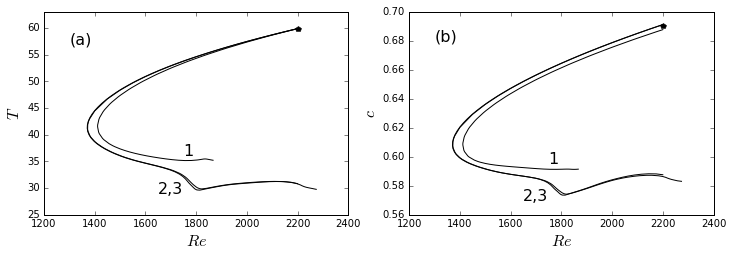
\includegraphics[width=0.9\linewidth]{local_contin.png}}
\caption{Продление модельного порыва в пространстве параметров $(T, c, \Re)$. Изображены зависимость периода изменения решения во времени $T$ и скорости его перемещения вдоль трубы $c$ от числа Рейнольдса $\Re$. Кривые 1, 2 и 3 соответствуют решениям, полученным на различных расчетных сетках. Черные точки соответствует исходному решению, принадлежащему сепаратрисе.}
\label{local_contin_pic}
\end{figure}

Как и на нижней ветви, на верхней решения остаются локализованными в пространстве и меняется во времени периодическим образом, однако они демонстрируют меньшую скорость перемещения вдоль трубы и меньший период изменения во времени. Для них характерна б\'{о}льшая интенсивность пульсаций и вторичных структур. Параметры решения на верхней ветви приближаются к параметрам турбулентного порыва. Это повышает ценность выводов, полученных при изучении решения  с верхней ветви. Если решения с нижней ветви находится на границе области притяжения турбулентного режима течения (на сепаратрисе), то решения с верхней ветви расположены внутри нее и могут участвовать в формировании турбулентного аттрактора\cite{Avila2013}. 

\begin{figure}
\center{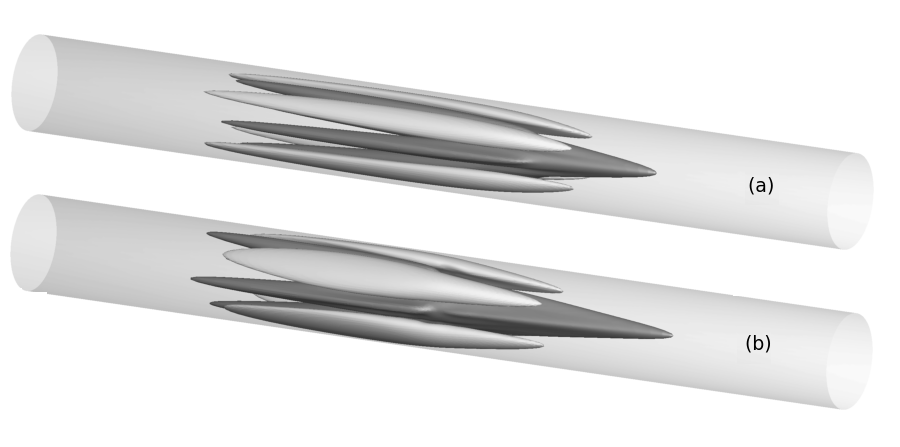
\includegraphics[width=0.9\linewidth]{3D_contin_cmp.png}}
\caption{Среднее поле скорости модельного порыва (1) и решения с верхней ветви при $\Re = 1700$ (2). Представлены изоповерхности, на которых скорость на 0.1 больше (красный) и меньше (синий) скорости в ламинарном течении. Поток направлен слева направо. }
\label{3D_contin_cmp_pic}
\end{figure}

Для того, чтобы установить параметры расчетной сетки, необходимые для адекватного воспроизведения решений на верхней ветви, решения были найдены на трех различных сетках. Исходная сетка построена при $L_x = 80$ и содержит $512 \times 32 \times 32$ ячеек в продольном, радиальном и угловом направлениях. Также решение было найдено на вдвое более подробной сетке, содержащей $1024 \times 64 \times 64$ ячеек при $L_x = 80$. Для того, чтобы продемонстрировать локализованность решения и его независимость от длины расчетной области, оно было найдено в расчетной области вдвое большей длины, при $L_x = 160$. В этом случае число ячеек в продольном направлении также удвоено, сетка содержит $1024 \times 32 \times 32$ ячеек. На рисунке \ref{local_contin_pic} приведены кривые для решений, полученных на всех трех сетках. Решения, полученные при $L_x = 80$ и $L_x = 160$, обозначенные на рисунке \ref{local_contin_pic} кривыми 2 и 3, практически совпадают друг с другом, что подтверждает пространственную локализованность решения. Характеристики решения, полученного на более подробной стеке, несколько отличаются, причем отличия тем выше, чем дальше решение от исходного. На рисунке \ref{local_contin_pic} подробной сетке соответствует кривая 1. Для более подробного исследования было выбрано решение с верхней ветви при $\Re = 1700$. Хотя при больших $\Re$ решения, полученные на различных сетках, повторяют качественные особенности друг друга, количественные отличия между ними нарастают, и мы не можем гарантировать, что использованных сеток достаточно для адекватного воспроизведения этих решений. Среднее поле скорости выбранного для дальнейшего исследования решения представлено на рисунке \ref{3D_contin_cmp_pic} внизу. Для сравнения изображено также среднее поле скорости модельного порыва вверху. Качественно структура решения не меняется, однако интенсивность полос на верхней ветви выше, чем на нижней. Период по времени выделенного решения можно оценить в $T = 35$, скорость его перемещения вдоль трубы в $c = 0.59$ (скорость перемещения турбулентного порыва вдоль трубы близка к $0.5$). 

Критическое число Рейнольдса, при котором рождается семейство решений, соответствующее модельному порыву, по результатом наших расчетов может быть оценено в $\Re^* = 1400$. В работе \cite{Avila2013} сообщается о близком значении $\Re^* = 1430$. 


\section{Характеристики модельного порыва с верхней ветви}

Продлевая решение, соответствующее модельному порыву, по числу Рейнольдса, удалось получить новое решение поставленной задачи, принадлежащее верхней ветви. Как и модельный порыв, оно локализовано в пространстве, и является условно периодическим по времени, но его характеристики оказываются ближе к характеристикам турбулентного порыва. Параметры выбранного для исследования решение: $\Re = 1700$, $T = 35$, $c = 0.59$. Особенности, выделенные при изучении модельного порыва, могут быть в полной мере обобщены на выделенное решение. 


\begin{figure}
\center{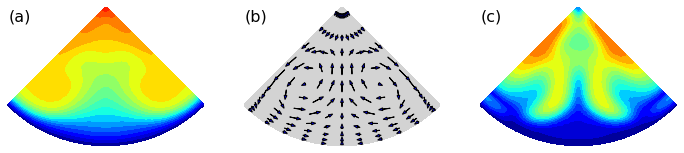
\includegraphics[width=0.9\linewidth]{local_ub_means.png}} 
\center{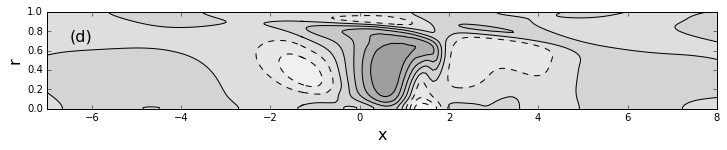
\includegraphics[width=0.9\linewidth]{local_ub_vel1.png}}
\caption{Поле скорости решения с верхней ветви. В сечении, где пульсации достигают наибольшей амплитуды, представлены: (a) --- $V_{x}$, (b) --- $(V_{r}, V_{\theta})$, (c) --- средняя по времени амплитуда $\v_n$; (d) --- мгновенное поле скорости $\v_n$ в сечении $\theta = 0$. }
\label{local_ub_means_pic}
\end{figure}


Как и в модельном порыве, в выделенном решении присутствуют полосы повышенной и пониженной скорости, вытянутые вдоль потока (смотри рисунок \ref{3D_contin_cmp_pic}). При разделении поля скорости решения $\v$ на среднюю $\V = \overline{\v}^t$ и пульсационную $\v_n = \v - \V$ составляющие, полосы попадают с среднюю составляющую движения. Продольная компонента среднего течения $V_x$ изображена на рисунке \ref{local_ub_means_pic}(a). Представлено только одно сечения, однако в других сечениях качественно картина не меняется. Полосы формируются за счет действия продольных вихрей, которые попадают в поперечную компоненту среднего течения $(V_r, V_\theta)$. Она в том же сечении представлена на рисунке \ref{local_ub_means_pic}(b). Пульсационная составляющая движения $\v_n$ имеет более сложную форму, чем в модельном порыв, однако в первую очередь она представляет бегущую вниз по потоку волну. Мгновенное поле скорости пульсационной составляющей движения $\v_n$ в продольном сечении $\theta = 0$ представлено на рисунке \ref{local_ub_means_pic}(d). На рисунке \ref{local_ub_means_pic}(с) представлена амплитуда пульсаций в том же сечении трубы. 

На рисунке \ref{amp_ub_pic} представлена средняя по сечению трубы амплитуда различных компонент движения. Как при исследовании модельного порыва, среднее течение разделено на двумерную $\V_{2D} = \overline{\V}^{\theta}$ и трехмерную $\V_{3D} = \V - \V_{2D}$ составляющие. Полосы и продольные вихри попадают в трехмерную составляющую движения. Качественно, распределение интенсивности различных компонент двжиения вдоль трубы в выделенном решении и в модельном порыве совпадают (смотри рисунок \ref{amp_pic}), однако все компоненты движения в выделенном решении имеют большую амплитуду. Интенсивность компонент движения $\V_{3D}$ выше примерно в двое. Интенсивность пульсаций $\v_n$ выше почти в четыре раза. На рисунке \ref{amp_ub_pic} представлены результаты, полученные на трех различных расчетных сетках, описанных в предыдущем разделе. Результаты, полученные на всех сетках, близки друг к другу, что подтверждает достаточность каждой из них для адекватного воспроизведения решения. 


\begin{figure}
\center{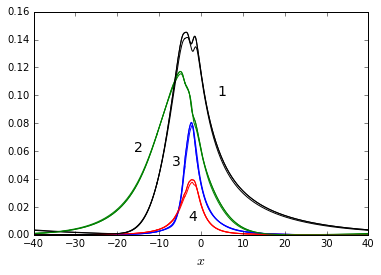
\includegraphics[width=0.6\linewidth]{amp_ub.png}}
\caption{Представлено распределение вдоль трубы амплитуды компонент движения решения с верхней ветви, $\Re = 1700$. Кривая 1 --- отклонение от течения Пуазейля поля скорости $V_{2D}$, кривые 2,3 --- продольная а поперечная компоненты поля скорости $\V_{3D}$, кривая 4 --- средняя по времени $\v_n$. Представлены результаты, полученных на трех расчетных сетках.}
\label{amp_ub_pic}
\end{figure}

Как в случае модельного порыва, в рассматриваемом случае среднее поле скорости решения на сепаратрисе оказывается линейно неустойчиво. Наиболее быстрорастущее возмущение, возникающее на среднем течении в рамках линеаризованных уравнений на него \eqref{lin_eq}, воспроизводит форму пульсационной составляющей движения. Оно может быть представлено в виде $\v'_1(x,r,\theta) e^{\lambda t}$. Инкремент нарастания приблизительно равен $\lambda = 0.014$. В силу относительной однородности среднего течения вдоль трубы, возникающее на нем возмущение близко к бегущей волне. Средняя по времени амплитуда возмущений $\v'_1$ представлена на рисунке \ref{ub_lin_pic}(a) в том же сечении, в котором пульсационная составляющая движения представлена на рисунке \ref{local_ub_means_pic}(c). Поле скорости $\v'_1$ в продольном сечении $\theta = 0$ представлена на рисунке \ref{ub_lin_pic}(b). В этом же сечении предсталвено мгновенное поле $\v_n$ на рисунке \ref{local_ub_means_pic}(d). Нет сомнений, что и в этом случае пульсационная составляющая движения возникает в результате потери линейной устойчивости средним течением. Отметим, что поле скорости $(V_x, 0, 0)$ оказывается устойчиво к малым возмущениям, соответствующий инкремент затухания приблизительно равен $\lambda = -0.009$. 

\begin{figure}
\center{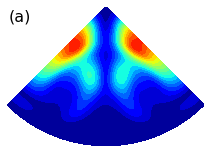
\includegraphics[width=0.3\linewidth]{ub_lin_cs.png} 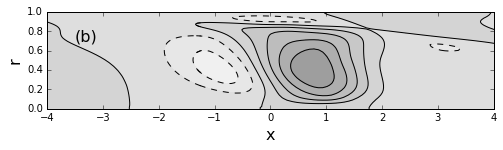
\includegraphics[width=0.6\linewidth]{ub_lin_ls.png}}
\caption{Наиболее быстрорастущее возмущение, возникающее на среднем течении в рамках линеаризованных уравнений \eqref{lin_eq}. Представлены: (a) --- амплитуда пульсаций в поперечном сечении трубы, как на рисунке \ref{local_ub_means_pic}(c); (b) --- мгновенное поле скорости в сечении $\theta = 0$, как на рисунке \ref{local_ub_means_pic}(d). }
\label{ub_lin_pic}
\end{figure}

\section{Выделенная из турбулентного течения бегущая волна в плоском канале}

\section{Выводы по главе}



\addcontentsline{toc}{chapter}{Заключение}
\chapter*{Заключение} 

%В заключении диссертации излагаются 1) итоги выполненного исследования, 2) выводы, 3) рекомендации, 4) перспективы дальнейшей разработки темы.

В геометрии течения в круглой трубе рассчитан модельный порыв --- условно периодическое решение уравнений Навье-Стокса с пространственно-локализованной структурой, являющееся предельным состоянием решения, эволюционирующего на сепаратрисе, разделяющей в фазовом пространстве области притяжения решений, соответствующих ламинарному и турбулентному режимам течения. Описана внутренняя структура модельного порыва и его основные характеристики. Показано, что модельный порыв воспроизводит ряд качественных особенностей турбулентных порывов, наблюдаемых в круглых трубах при переходных числах Рейнольдса. Также, как в турбулентном порыве, в модельном порыве можно выделить вытянутые вдоль потока полосы повышенной и пониженной скорости, но если в первом случае эти полосы перемещаются вдоль стенки и их сплошность разрываются флуктуирующей составляющей движения, то во втором случае они сохраняют свое положение в пространстве и подвержены лишь небольшим колебаниям. Простое временное поведение модельного порыва позволило выполнить его детальное исследование. Полученные при исследовании модельного порыва результаты, мы полагаем, будут полезны для понимания турбулентного порыва. 

Установить универсальность наблюдаемых в модельном порыве закономерностей движения позволяет анализ других инвариантных решений Навье-Стокса, рассчитанных в работе. Методом продолжения по параметру рассчитано соответствующее модельному порыву семейство условно периодических решений уравнений Навье-Стокса с пространственно-локализованной структурой. В частности, найдены решения, оказывающиеся по ряду качественных характеристик ближе к турбулентному порыву, чем модельный порыв. Можно ожидать, что выводы, сделанные на основе исследования модельного порыва и этих решений имеют большее отношение к турбулентному порыву, чем выводы, сделанные при исследовании только модельного порыва. Также в геометрии течения в круглой трубе и течения в плоском канале найдено три семейства решений, имеющих вид бегущей волны. Анализ всех найденных решений позволяет сформулировать идеализированный цикл поддержания колебаний в такого рода решениях. 

Поле скорости каждого решения может быть представлено в виде суммы средней и пульсационной составляющих. Во всех исследованных решениях в среднем течении существуют вытянутые вдоль потока полосы повышенной и пониженной скорости, чередующиеся в угловом (поперечном) направлении. В случае решения в виде бегущей волны среднее поле скорости не зависит от продольной координаты и, соответственно, полосы имеют неограниченную протяженность. В случае решений с пространственно-локализованной структурой полосы имеют ограниченную протяженность. Возбуждение пульсаций связано с линейной неустойчивостью среднего течения. Колебания оказываются сконцентрированы в промежуточных областях между соседними полосами повышенной и пониженной скорости. В этих областях распределение среднее продольной скорости имеет точки перегиба, если рассматривать его как функцию угловой (поперечной) координаты, что позволяет связать неустойчивость среднего течения с неустойчивость струйных течений с точками перегиба. За поддержание полос ответственны продольные вихри, перемещающие жидкость в нормальной к основному потоку плоскости. 

Существенным результатом работы является описание нелинейного механизма поддержания продольных вихрей. Показано, что во всех решениях продольные вихри образуются в результате нелинейного взаимодействия пульсаций продольной скорости и пульсаций продольной завихренности. Пульсации продольной завихренности в области расположения продольных вихрей образуются за счет сжатия и растяжения существующих вихревых трубок пульсациями продольной скорости, что обеспечивает необходимую для поддержания продольных вихрей согласованность фаз между этими пульсациями. Отметим, что продольные вихри образуются в областях возникновения пульсаций, между полосами повышенной и пониженной скорости, так как именно в этих областях пульсации имеют наибольшую амплитуду и средняя скорость жидкость совпадает с фазовой скоростью пульсаций, что необходимо для образования пульсаций продольной завихренности описанным механизмом. Таким образом, продольные вихри образуются в промежуточной области между полосами повышенной и пониженной скорости, оказываясь расположенными наиболее удачным образом для поддержания существования этих полос. 

Наиболее быстрорастущее решение линейной задачи устойчивости среднего течения также воспроизводит описанный механизм поддержания продольных вихрей, но только в том случае, если при анализе среднего течения на устойчивость учтена не только продольная но и поперечная компоненты средней скорости. Принято считать, что поперечная компонента движения, поддерживая угловую (поперечную) неоднородность среднего течения, не оказывает существенного влияния на характеристики устойчивости среднего течения. Мы видим, что учет поперечной компоненты среднего течения необходим для адекватного воспроизведения механизма поддержания колебаний. 

Полосчатые структуры являются неотъемлемым элементом всех сценариев самоподдержания турбулентности в пристенных течениях, что говорит о вероятной близости выделенного в работе механизма с механизмом самоподдержания однородной (нелокализованной) пристенной турбулентности. На следующем этапе выполнения работы необходимо установить применимость сделанных выводов к турбулентному порву, и к более широкому классу пристенных турбулентных течений. Для этого, по-видимому, необходимо разработать метод промежуточного осреднения, позволяющий выделить в реальном турбулентном течении крупномасштабные и мелкомасштабные структуры. Это позволит обобщить рассуждения, применяемые в работе, на такого рода течения. Имея представления о механизме поддержания колебаний можно предложить эффективные стратегии управления турбулентными течениями с целью снижения или увеличения интенсивности колебаний. Эти стратегии также могут быть опробованы на реальных пристенных турбулентных течениях (численно), и в зависимости от их эффективности могут быть сделаны выводы о роли выделенных механизмов в поддержании такого рода режимов течения. В случае, если разработанные стратегии управления турбулентными потоками покажут себя эффективными, они имеют собственную значительную ценность. 







\newcommand{\listpub}{Список литературы}
\renewcommand{\bibname}{\listpub}

\phantomsection
\addcontentsline{toc}{chapter}{\tocsecindent{\listpub}}
\bibliography{bib/base,bib/rus,bib/books,bib/my}


\end{document}
